% !TeX program = pdflatex
% Target ICML 2027; see TEMPLATE_PROVENANCE.txt for official-style availability.
\documentclass{article}
\PassOptionsToPackage{table}{xcolor}
\usepackage{hyperref}
\usepackage{icml2027_draft}
\usepackage[utf8]{inputenc}
\usepackage[T1]{fontenc}
\usepackage{xurl}
\usepackage{booktabs}
\usepackage{amsfonts,amsmath,amssymb,amsthm,mathtools}
\usepackage{nicefrac}
\usepackage{mathrsfs}
\usepackage{microtype}
\usepackage{xcolor}
\usepackage{graphicx}
\usepackage{subcaption}
\usepackage{wrapfig}
\usepackage{array}
\usepackage{tabularx}
\usepackage{pifont}
\usepackage{enumitem}
\usepackage{makecell}
\setlength{\emergencystretch}{1em}
\usepackage{longtable}
\usepackage{placeins}
\usepackage{float}
\usepackage{adjustbox}
\usepackage{multirow}

\newtheorem{theorem}{Theorem}[section]
\newtheorem{remark}[theorem]{Remark}
\newtheorem{lemma}[theorem]{Lemma}
\newtheorem{proposition}[theorem]{Proposition}
\newtheorem{assumption}[theorem]{Assumption}
\newtheorem{definition}[theorem]{Definition}
\newtheorem{corollary}[theorem]{Corollary}
\newcommand{\HH}{\mathbb{H}}
\newcommand{\RR}{\mathbb{R}}
\newcommand{\cL}{\mathcal{L}}
\newcommand{\Exp}{\operatorname{Exp}}
\newcommand{\Log}{\operatorname{Log}}
\newcommand{\grad}{\operatorname{grad}}
\newcommand{\PT}{\mathcal{P}}
\newcommand{\Proj}{\operatorname{Proj}}
\newcommand{\softplus}{\operatorname{softplus}}
\newcommand{\arcosh}{\operatorname{arcosh}}
\newcommand{\norm}[1]{\left\lVert #1\right\rVert}
\newcommand{\inner}[2]{\langle #1,#2\rangle_{\cL}}
\newcommand{\Kstd}{K_{\mathrm{std}}}
\definecolor{oursbg}{RGB}{230,244,233}
\definecolor{oursgoodbg}{RGB}{198,232,205}
\definecolor{checkgreen}{RGB}{21,128,61}
\definecolor{crossred}{RGB}{190,35,45}
\definecolor{rwblue}{HTML}{1761A0}
\definecolor{rwgreen}{HTML}{197647}
\definecolor{rwred}{HTML}{B13B37}
\definecolor{rwgray}{HTML}{F1F3F5}
\newcommand{\rwcheck}{\textcolor{rwgreen}{\ding{51}}}
\newcommand{\rwcross}{\textcolor{rwred}{\ding{55}}}
\newcommand{\rwna}{\textcolor{gray}{\textemdash}}


\icmltitlerunning{HyperbolicMomentum: Curvature-Adaptive Manifold Optimization}
\begin{document}
\twocolumn[
\icmltitle{HyperbolicMomentum: Curvature-Adaptive Momentum\\for Hierarchical Neural Optimization}
\begin{icmlauthorlist}
\icmlauthor{Anonymous Authors}{anon}
\end{icmlauthorlist}
\icmlaffiliation{anon}{Anonymous Institution}
\icmlcorrespondingauthor{}{}
\icmlkeywords{Riemannian optimization, hyperbolic geometry, momentum, learnable curvature}
\vskip 0.3in
]
\printAffiliationsAndNotice{}

\begin{abstract}
We introduce \emph{HyperbolicMomentum}, a Lorentz-model optimizer that combines grouped learnable curvature, curvature-normalized geodesic steps, and consistent momentum transport across tangent spaces and curvature changes. We derive an exact curvature-independent sensitivity certificate for normalized steps, sharp normalization and heterogeneity constants with equality cases, and conditional convergence, full-state stability, and generalization bounds. In complete 2000-update synthetic experiments, matched five-initialization searches selected by validation reduce held-out distortion by $2.94\%$ in a stationary hierarchy and $3.31\%$ and $5.02\%$ under $2\times$ and $8\times$ smooth distance drift, relative to selected normalized fixed-curvature momentum. These are selected positive conditions from a six-case matrix with mixed outcomes, and the radius constraint permits curvature-dependent physical capacity. The omitted-transport ablation remains close, so training scores do not isolate a transport benefit. A separate operator experiment does: compatible transport keeps the maximum FP32 canonical momentum error below $3.2\times10^{-6}$, whereas point-only transport yields final errors of $1.70\%$--$4.94\%$ under prescribed drift. Historical knowledge-graph results supply exploratory curvature evidence. All evaluated conditions, including negative and tied results, remain available in the complete comparison appendix, and the 705 retained full-length configurations and all delayed test evaluations are complete.
\end{abstract}

\section{Introduction}

Hierarchical structure is one of the recurring reasons that Euclidean representation learning becomes inefficient. Taxonomies branch exponentially with depth, lexical relations mix tree-like and symmetric components, knowledge graphs combine multi-relational hierarchies with many-to-many relations, and graph or language representations often need to place coarse categories, fine instances, and lateral neighborhoods in the same embedding system. Hyperbolic representation learning addresses this mismatch by using negative curvature, whose volume growth matches trees more naturally than Euclidean space \citep{nickel2017poincare,nickel2018lorentz,chami2019hgcn,tifrea2019poincare,balazevic2019poincare}. In examples such as WordNet taxonomies, Freebase relation graphs, and synthetic trees with heterogeneous branching, the relevant question is not only whether hyperbolic space helps, but which curvature each structural component should use during optimization.

\begin{table*}[t]
\centering
\caption{\textbf{HyperbolicMomentum update.} Each group has a dedicated Lorentz manifold. The main path updates the point and tangent momentum; the slower branch changes curvature and maps both states. The curvature derivative is total at fixed canonical point, as in Eq.~\eqref{eq:total-curv-gradient}.}
\label{tab:method-overview}
\footnotesize\setlength{\tabcolsep}{4.2pt}\renewcommand{\arraystretch}{1.12}
\begin{tabularx}{\linewidth}{l l X}
\toprule
Stage & State or operation & Geometric role \\
\midrule
\multicolumn{3}{l}{\textit{Tangent-state and geodesic update}} \\
Gradient & $\widehat g_{g,t}=\grad_{x_g}\mathcal J$ & Form a tangent direction at the current point. \\
Momentum & $\widetilde m_{g,t}=\beta m_{g,t}+(1-\beta)\widehat g_{g,t}$ & Average directions in the same tangent space. \\
\rowcolor{oursbg}
Normalized step & $\eta^{\rm geo}_{g,t}=\eta_t/(1+\gamma\sqrt{K_{g,t}}\|\widetilde m_{g,t}\|)$ & Control the curvature--momentum scale. \\
Geodesic move & $x_{g,t+1/2}=\Exp_{x_{g,t}}^{K_{g,t}}(-\eta^{\rm geo}_{g,t}\widetilde m_{g,t})$ & Move the point on its current manifold. \\
Tangent transport & $m_{g,t+1/2}=\PT_{x_{g,t}\to x_{g,t+1/2}}^{K_{g,t}}\widetilde m_{g,t}$ & Carry memory to the new base point. \\
\midrule
\multicolumn{3}{l}{\textit{Slow curvature update and compatible joint-state map}} \\
\rowcolor{oursbg}
Learn curvature & $\widehat h_{g,t}=\partial_{c_g}F(q_t,u_t)$; Eq.~\eqref{eq:k-step-main} & Use the total derivative, with bounded log drift in implementation. \\
\rowcolor{oursbg}
Map joint state & $a_g=\sqrt{K_{g,t}/K_{g,t+1}}$; Eq.~\eqref{eq:xcurv-main} & Scale both point and momentum by $a_g$; restore tangency numerically. \\
\bottomrule
\end{tabularx}
\end{table*}


Table~\ref{tab:method-overview} summarizes the coupled update. A useful distinction is between fixed-manifold optimization, architectural curvature learning, and consistency of optimizer state when curvature changes. Recent curvature-aware Lorentz optimization already addresses the last issue using origin-tangent remapping~\citep{bdeir2025robust}. Our study concerns the particular homothetic state map, grouped slow curvature updates, normalized geodesic step, and their conditional analysis.


A fixed-curvature optimizer cannot adapt its manifold to different structural groups. Riemannian stochastic gradient descent provides a principled first-order update on manifolds \citep{bonnabel2013sgd,zhang2016geodesic}, and Riemannian adaptive methods extend adaptive optimization to curved spaces \citep{becigneul2019radam}. Yet a fixed-curvature optimizer cannot adapt when one relation behaves like a taxonomic branch, another relation behaves like a symmetric neighborhood, and a third relation behaves like a high-degree multi-relational association. Knowledge graph baselines such as TransE and RotatE illustrate how strongly relation type shapes the geometry of a representation problem \citep{bordes2013transe,sun2019rotate}; hyperbolic KG methods further show that relation-aware curvature can matter \citep{balazevic2019poincare}. A second requirement is geometric: momentum vectors live in tangent spaces. The vector carried from step $t-1$ belongs to $T_{x_{t-1}}\HH^d_{-K}$, whereas the current gradient belongs to $T_{x_t}\HH^d_{-K}$, so adding them without parallel transport has no intrinsic meaning. If $K$ itself changes, then both the base point and the metric radius change, making a point-only curvature update incomplete for architectures in which each group has its own manifold.

This paper studies the optimization problem that appears when these two requirements coincide. We ask whether a hierarchical model should learn \textbf{one curvature per structural group}, whether the geodesic step should be normalized by the local curvature-momentum scale, and when a \textbf{cross-curvature momentum state} is actually meaningful. The answer is deliberately nuanced. Historical unfiltered, tail-only experiments with Euclidean Adam provide exploratory evidence for grouped learnable curvature: on WN18RR, B4 improves Hits@10 by $+4.1\%$ and loss by $-2.8\%$ over fixed curvature B3, while MRR is positive but sensitive to the moving-average window. On FB15k-237, the same mechanism gives a different metric profile: MRR improves by $+2.2\%$ and Hits@1 by $+3.1\%$, but Hits@10 is almost unchanged at $+0.1\%$. Thus the shared positive KG signal is MRR, while which Hits metric benefits depends on the dataset.

We present \textbf{HyperbolicMomentum}, an optimizer in the Lorentz model with three mechanisms: grouped learnable curvature, curvature-normalized geodesic steps, and cross-curvature parallel-transport momentum. The method is motivated by one controlling geometric quantity. The product $\sqrt{K}R$ governs capacity, conditioning, and stability over radius $R$, while $\sqrt{K}\eta\|m\|$ governs exponential-map distortion during an optimization step. Our theory makes this trade-off explicit through exact homothety and Jacobi-field identities, a quantitative heterogeneity bound, error-explicit two-block convergence, momentum tracking, constrained curvature stationarity, finite-precision propagation, and augmented-state stability with an explicit training-time factor. Table~\ref{tab:curvatures} lists the relation-dependent curvature states: WN18RR learns a wide relation-dependent curvature spread, whereas FB15k-237 learns a much smaller spread consistent with weaker hierarchy.

\begin{table*}[t]
\centering
\caption{\textbf{Learned relation curvatures.} Historical B4 values. All 11 WN18RR relations and the 15 displayed FB15k-237 relations are retained; the fixed baseline is $K=1$. Curvature magnitude is a parameter, not a performance ranking.}
\label{tab:curvatures}
\footnotesize\setlength{\tabcolsep}{4.2pt}\renewcommand{\arraystretch}{1.12}
\begin{adjustbox}{max width=\linewidth}
\begin{tabular}{lrrr}
\toprule
WN18RR relation & $K$ & FB15k-237 relation & $K$ \\
\midrule
derivationally related form & 2.0000 & award/nominee & 1.8371 \\
member meronym & 1.5823 & film/release region & 1.3486 \\
hypernym & 1.4173 & award/winner (A) & 1.3449 \\
has part & 1.3050 & award/nominee$\to$award & 1.2725 \\
instance hypernym & 1.2220 & music/genre$\to$artists & 1.1832 \\
verb group & 1.0938 & person/profession & 1.1817 \\
also see & 1.0888 & film/genre & 1.1754 \\
synset domain topic of & 1.0754 & award/nominees for & 1.1678 \\
member of domain region & 1.0170 & actor/filmography & 1.1677 \\
member of domain usage & 1.0092 & award/winners (B) & 1.1435 \\
similar to & 1.0084 & film/other crew & 1.1421 \\
-- & -- & award/nominated for & 1.1338 \\
-- & -- & person/nationality & 1.1093 \\
-- & -- & work/awards won & 1.1034 \\
-- & -- & sports/team roster & 1.0966 \\
\bottomrule
\end{tabular}
\end{adjustbox}
\end{table*}


The contributions are as follows, stated in prose to match the empirical evidence. First, we formulate HyperbolicMomentum as a single Lorentz-model algorithm that learns grouped curvatures and uses curvature-normalized geodesic steps, with cross-curvature momentum transport included only when the architecture supplies a dedicated manifold per group. Second, we derive an exact curvature-independent sensitivity certificate for normalized geodesic steps, optimal normalization derivative constants, and a sharp Hessian-weighted heterogeneity bound. The convergence proof preserves finite-horizon martingale weights, while the statistical analysis combines the full state-comparison matrix with stability concentration and entropy chaining. Third, we separate historical curvature ablations from new full-data comparisons and 2000-update controlled drift experiments. The complete matched-initialization search yields held-out distortion reductions of $2.94\%$, $3.31\%$, and $5.02\%$ relative to selected normalized fixed curvature in the stationary, $2\times$ smooth-drift, and $8\times$ smooth-drift conditions. These are the stronger conditions in a six-case matrix; the point-only transport ablation remains close. These conditional gains combine scale adaptation with the physical-distance budget under a canonical-radius cap; they do not imply a uniform advantage across all conditions. Direct operator measurements separately verify the sensitivity and momentum-consistency predictions. Fourth, we document structural curvature differentiation: WN18RR differentiates across relations, FB15k-237 by relation complexity with a four-times smaller $K$ spread, and synthetic trees by branching rate.

\section{Related Work}
\label{sec:related-work}

\paragraph{Hyperbolic representations and learned curvature.}
Poincar\'{e} embeddings use negative curvature for compact hierarchical representations, while Lorentz embeddings provide an alternative model with closed-form geodesic operations~\citep{nickel2017poincare,nickel2018lorentz}. Learning curvature is already established: product-space embeddings jointly learn geometry across factors~\citep{gu2019mixed}, and HGCN learns a curvature at each graph-convolution layer~\citep{chami2019hgcn}. For knowledge graphs, MuRP provides a hyperbolic relational model~\citep{balazevic2019poincare}, while RotH and AttH learn relation-specific curvatures together with isometric transformations~\citep{chami2020atth}. Poincar\'{e} GloVe extends hyperbolic representation learning to lexical co-occurrence~\citep{tifrea2019poincare}. Grouped or relation-specific curvature is therefore a precedent, rather than a novelty claim of this paper.

\paragraph{Riemannian optimization and optimizer memory.}
RSGD establishes stochastic optimization directly on a manifold~\citep{bonnabel2013sgd}; curvature-dependent first-order analysis characterizes geodesically convex objectives~\citep{zhang2016geodesic}. Riemannian Adam and AMSGrad maintain adaptive statistics on a product manifold and transport first-moment information between tangent spaces~\citep{becigneul2019radam}. More recent adaptive frameworks analyze minibatch size and constant or diminishing steps on embedded manifolds~\citep{sakai2024adaptive}. These are important fixed-manifold foundations. Our analysis additionally tracks a learned curvature coordinate, including the gradient induced by identifying points through a curvature-dependent homothety. It retains the different representation and curvature step weights instead of assigning both blocks the same rate by default.

\paragraph{Curvature-aware state mapping: the closest optimization precedent.}
\citet{bdeir2025robust} already identify mismatches caused by updating curvature while retaining stale manifold parameters and optimizer states. Their curvature-aware scheme updates parameters and transports gradients and momentum through the origin tangent space; it is combined with Riemannian AdamW and radius rescaling. We therefore do not claim to introduce cross-curvature optimizer-state consistency. HyperbolicMomentum instead studies a homothetic point-and-momentum map, grouped slow curvature updates, and a curvature--momentum normalized geodesic step. The distinction is the chosen coupled update and its error-explicit analysis; the homothety itself also has precedents discussed by that work. Its behavior relative to origin-tangent remapping requires a matched empirical comparison, which the current experiments do not supply.

\begin{table*}[!ht]
\centering
\caption{\textbf{Mechanisms in related work.} Keywords identify the design; checks identify properties of the cited formulation. Curvature learning and cross-curvature optimizer-state mapping both have prior art. The final column denotes our specific curvature--momentum step normalization, not all forms of adaptive learning rates or radius control.}
\label{tab:related-work-features}
\begingroup
\footnotesize
\setlength{\tabcolsep}{4.2pt}
\renewcommand{\arraystretch}{1.12}
\begin{tabularx}{\linewidth}{@{}>{\raggedright\arraybackslash}p{.215\linewidth}>{\raggedright\arraybackslash}p{.225\linewidth}*{5}{>{\centering\arraybackslash}X}@{}}
\toprule
\textbf{Method / family} & \textbf{Core mechanism} & \textbf{Learned $K$} & \textbf{$K$ scope} & \textbf{Tangent memory} & \textbf{Cross-$K$ memory} & \textbf{Step control} \\
\midrule
\rowcolor{rwgray}
\multicolumn{7}{@{}l}{\textit{Optimization on a prescribed geometry}} \\
RSGD~\citep{bonnabel2013sgd} & Stochastic tangent descent & \rwcross & Fixed & \rwcross & \rwna & \rwcross \\
Lorentz embeddings~\citep{nickel2018lorentz} & Hyperboloid Exp update & \rwcross & Fixed & \rwcross & \rwna & \rwcross \\
RAdam / RAMSGrad~\citep{becigneul2019radam} & Transported adaptive moments & \rwcross & Fixed & \rwcheck & \rwna & \rwcross \\
\addlinespace[2pt]
\rowcolor{rwgray}
\multicolumn{7}{@{}l}{\textit{Learning the representation geometry}} \\
Product spaces~\citep{gu2019mixed} & Mixed-curvature factors & \rwcheck & Factor & \rwna & \rwna & \rwcross \\
HGCN~\citep{chami2019hgcn} & Hyperbolic message passing & \rwcheck & Layer & \rwna & \rwna & \rwcross \\
RotH / AttH~\citep{chami2020atth} & Isometries + attention & \rwcheck & Relation & \rwcross & \rwcross & \rwcross \\
\addlinespace[2pt]
\rowcolor{rwgray}
\multicolumn{7}{@{}l}{\textit{Coupling curvature changes to optimizer state}} \\
Curvature-aware Lorentz~\citep{bdeir2025robust} & Origin-tangent remapping + RAdamW & \rwcheck & Manifold & \rwcheck & \rwcheck & \rwcross \\
\midrule
\rowcolor{oursbg}
\textbf{HyperbolicMomentum} & \textbf{Homothety + controlled Exp step} & \rwcheck & Group & \rwcheck & \rwcheck & \rwcheck \\
\bottomrule
\end{tabularx}
\par\vspace{4pt}
\begin{minipage}{\linewidth}
\scriptsize
\rwcheck\ present; \rwcross\ absent in the listed formulation; \rwna\ not specified as a core optimizer mechanism, or not applicable for fixed $K$.
\emph{Tangent memory}: a first-moment state attached to moving manifold points; ordinary Euclidean Adam states in origin coordinates are not counted.
\emph{Cross-$K$ memory}: an explicit rule for adapting that state when curvature changes; mappings of neural activations between layers are not counted.
\emph{Normalized step}: $\eta^{\rm geo}=\eta/(1+\gamma\sqrt K\|\widetilde m\|)$, which bounds $\sqrt K\|v\|$; Adam preconditioning and embedding-radius clipping are distinct mechanisms.
The row for our method describes its grouped-manifold formulation, not the historical shared-entity KG implementation. No check implies empirical superiority.
\end{minipage}
\endgroup
\end{table*}


\paragraph{The map being compared.}
The origin-tangent point map has the form
$\Exp_{o_{K'}}^{K'}\!\circ\Log_{o_K}^{K}$ and retains the physical radial coordinate. Our map is
$\Psi_{K\to K'}(x)=\sqrt{K/K'}\,x$, with differential
$D\Psi(v)=\sqrt{K/K'}\,v$; it retains the canonical state
$q=\sqrt Kx$, $p=\sqrt Km$ while scaling physical distances.
These invariants are different. Neither map implies a universal performance ordering. Table~\ref{tab:related-work-features} separates architectural curvature learning, transported tangent memory, and changes of the geometry itself, rather than assigning every hyperbolic model the same optimizer.

\paragraph{Generalization and evidence boundaries.}
Replace-one stability links coupled optimization trajectories to expected generalization under an appropriate sampling model~\citep{hardt2016stability}. Our conditional bound exposes its curvature-radius and cumulative-step dependence and distinguishes fixed i.i.d. data from graph dependence or continual-learning shift. Historical KG measurements in this paper are exploratory fixed-versus-learned-curvature Adam comparisons; they are not matched optimizer comparisons against RotH/AttH or curvature-aware RAdamW. The table records mechanisms, while the experiment section separately records which comparisons were actually run.

\section{Preliminaries and Problem Setup}

We work in the Lorentz model because it gives closed-form geodesics and parallel transport. For $K>0$, the $d$-dimensional hyperbolic space of sectional curvature $-K$ is
\begin{equation}
\begin{gathered}
\HH_{-K}^{d}=\{x\in\RR^{d+1}:\inner{x}{x}=-1/K,\;x_0>0\},\\
\inner{x}{y}=-x_0y_0+\sum_{i=1}^{d}x_iy_i .
\end{gathered}
\end{equation}
The tangent space at $x$ is $T_x\HH_{-K}^{d}=\{v:\inner{x}{v}=0\}$ with norm $\|v\|_x=\sqrt{\inner{v}{v}}$. The exponential map is
\begin{equation}
\Exp_x^K(v)=\cosh(\sqrt{K}r)x+\frac{\sinh(\sqrt{K}r)}{\sqrt{K}r}v,\qquad r=\|v\|_x,
\label{eq:exp-main}
\end{equation}
with the usual convention at $r=0$. This formula shows why the product $\sqrt{K}r$ is central: it is the argument of the hyperbolic sine and cosine terms that control both useful volume growth and harmful numerical amplification.

For momentum, the previous tangent vector must be moved before it can be combined with the current gradient. Along the geodesic from $x$ to $y$ at fixed curvature, the Lorentz parallel transport of $v\in T_x\HH^d_{-K}$ is
\begin{equation}
\PT_{x\to y}^{K}(v)=v+\frac{K\inner{y}{v}}{1-K\inner{x}{y}}(x+y),
\label{eq:pt-main}
\end{equation}
which lies in $T_y\HH^d_{-K}$ and preserves the Lorentz norm. When curvature changes from $K$ to $K'$, the natural Lorentz rescaling maps points and tangent vectors as $\Psi_{K\to K'}(x)=\sqrt{K/K'}x$ and $\mathcal{C}_{K\to K'}(v)=\sqrt{K/K'}v$. These maps preserve the hyperboloid constraint and give the first-order cross-curvature consistency used by the optimizer.

The learning problem has $G$ structural groups. Each group $g$ has a parameter point $x_{g,t}\in\HH^{d_g}_{-K_{g,t}}$, a momentum vector $m_{g,t}\in T_{x_{g,t}}\HH^{d_g}_{-K_{g,t}}$, and a log-curvature coordinate $u_{g,t}=\log K_{g,t}$ implemented with a positive softplus parameterization and clipping to $[K_{\min},K_{\max}]$. The joint objective is
\begin{equation}
\mathcal{J}(x,u)=F(x,e^u)+\lambda_u\sum_g (u_g-u_{\mathrm{ref}})^2.
\label{eq:joint-main}
\end{equation}
The regularizer is not a claim that all curvatures should equal the reference; it is a numerical guard against runaway curvature. In the KG experiments, WN18RR reaches a boundary-like regime near $K=2$ for the highest-curvature relation, whereas synthetic runs often remain in an interior regime. The distinction matters for theory and is stated explicitly in Section~\ref{sec:theory}.

The experimental method labels are fixed throughout the paper. B3 is fixed-curvature Riemannian momentum with $K=1$. B4 adds grouped learnable curvature and maps points as curvature changes. B5 is the full HyperbolicMomentum variant with learnable curvature, curvature-normalized geodesic steps, and cross-curvature momentum transport. In shared-entity KG architectures, relation-specific curvature is used at scoring time while entity embeddings are shared across relations; therefore B5's cross-curvature momentum mechanism has no coherent home manifold and the KG comparison is interpreted as B4 versus B3, not as evidence for B5 beating B4.

\section{Methodology}
\label{sec:methodology}
Table~\ref{tab:method-overview} shows the main update and its slower curvature branch. The current momentum is stored at the current point; geodesic transport and cross-curvature mapping occur after the step, before the next iteration.


The intuition behind HyperbolicMomentum is that curvature should be treated like a slowly changing geometric state, not like a static hyperparameter. A high-curvature group can represent rapid hierarchical expansion, but the same high curvature makes exponential-map perturbations and finite-precision residuals larger. The optimizer therefore learns $K_g$ only on a slower timescale, rescales geodesic steps by the local curvature-momentum magnitude, and transports momentum only when the model architecture gives that momentum a well-defined manifold on which to live.

For each group $g$, the stochastic Riemannian gradient is $\widehat g_{g,t}=\grad_{x_g}\mathcal{J}(x_t,u_t)$ and the stochastic curvature gradient is $\widehat h_{g,t}=\partial_{c_g}F(q_t,u_t)$, including the point-rescaling derivative in Eq.~\eqref{eq:total-curv-gradient}. The stored momentum $m_{g,t}$ already belongs to the current tangent space because the previous step transported it. The update averages this state with the current gradient:
\begin{equation}
\widetilde m_{g,t}=\beta m_{g,t}+(1-\beta)\widehat g_{g,t}.
\label{eq:momentum-main}
\end{equation}
This equation is the Riemannian analogue of Euclidean momentum. Transport is performed after the geodesic update below and across curvature changes; applying it again at the next iteration would double-count the state movement.

The geodesic step uses a curvature-normalized learning rate,
\begin{equation}
\chi_{g,t}=\sqrt{K_{g,t}}\|\widetilde m_{g,t}\|_{x_{g,t}},\qquad
\eta^{\mathrm{geo}}_{g,t}=\frac{\eta_t}{1+\gamma\chi_{g,t}}.
\label{eq:eta-main}
\end{equation}
The quantity $\chi_{g,t}$ is dimensionless. It is exactly the part of the exponential map argument that grows with both curvature and momentum norm, so the denominator prevents large-$K$ groups from taking disproportionately distorted geodesic steps. The parameter update is
\begin{equation}
\begin{gathered}
x_{g,t+\frac12}=\Exp_{x_{g,t}}^{K_{g,t}}(-\eta^{\mathrm{geo}}_{g,t}\widetilde m_{g,t}),\\
m_{g,t+\frac12}=\PT_{x_{g,t}\to x_{g,t+\frac12}}^{K_{g,t}}(\widetilde m_{g,t}).
\end{gathered}
\label{eq:x-step-main}
\end{equation}
The first equation moves the parameter on the manifold. The second keeps the velocity state aligned with the new base point, so that the next iteration starts with a tangent vector at the correct point.

Curvature is updated after the geodesic step with a slower step size $\rho_t$:
\begin{equation}
K_{g,t+1}=K_{\min}+\softplus(c_{g,t}-\rho_t\widehat h_{g,t}).
\label{eq:k-step-main}
\end{equation}
When the architecture has a dedicated manifold per group, both the point and momentum are then mapped to the new curvature:
\begin{equation}
\begin{gathered}
x_{g,t+1}=\sqrt{\frac{K_{g,t}}{K_{g,t+1}}}\,x_{g,t+\frac12},\\
m_{g,t+1}=\Proj_{T_{x_{g,t+1}}}\left[\sqrt{\frac{K_{g,t}}{K_{g,t+1}}}\,m_{g,t+\frac12}\right].
\end{gathered}
\label{eq:xcurv-main}
\end{equation}
The point rescaling enforces $\langle x,x\rangle_{\mathcal L}=-1/K_{g,t+1}$. The projected tangent rescaling corrects finite-precision tangency error. We do not assert that Lorentz projection contracts arbitrary ambient vectors, since the ambient bilinear form is indefinite. In the experiments, numerical method M1 applies this projection at every step in pure FP32.

\begin{center}
\fbox{\begin{minipage}{0.94\linewidth}
\textbf{Algorithm 1: HyperbolicMomentum update for group $g$.} Given $(x_{g,t},m_{g,t},K_{g,t})$, compute $\widehat g_{g,t}$ and $\widehat h_{g,t}$; average the current tangent momentum with Eq.~\eqref{eq:momentum-main}; compute the curvature-normalized step in Eq.~\eqref{eq:eta-main}; move $x$ and momentum with Eq.~\eqref{eq:x-step-main}; update curvature with Eq.~\eqref{eq:k-step-main}; and, in grouped-manifold architectures, map both point and momentum to $K_{g,t+1}$ with Eq.~\eqref{eq:xcurv-main}. In shared-entity KG architectures, the learnable-curvature and normalized-step mechanisms remain valid, but the cross-curvature momentum step is not interpreted as a separate B5 advantage.
\end{minipage}}
\end{center}

\section{Theory}
\label{sec:theory}
The analysis uses one geometric identification to connect optimization and generalization. Canonical coordinates fix the state space while exposing curvature as a preconditioner; exact Jacobi operators then quantify the effect of normalization. A predictable parallel frame preserves martingale orthogonality in the momentum proof. Finally, the full comparison matrix yields a stability certificate through Collatz--Wielandt, and chaining controls hypothesis complexity. The appendix supplies complete proofs and distinguishes sharp constants and equality cases from sufficient asymptotic rates.

Write
\begin{gather}
 \mathcal Q=\prod_{g=1}^G(H_1^{d_g})^{n_g},\quad u_g=\log K_g,\\
 q_g=\sqrt{K_g}x_g,\qquad p_g=\sqrt{K_g}m_g,\\
 F(q,u)=\widetilde{\mathcal J}((e^{-u_g/2}q_g)_g,u),\\
 A(u)=\operatorname{diag}(K_gI)_{g=1}^G,\\
 g_t=\operatorname{grad}_qF(q_t,u_t),\quad b_t=\nabla_uF(q_t,u_t),\\
 N_\gamma(v)=\frac{v}{1+\gamma\|v\|}.
\end{gather}
The main results use normalization blocks contained in individual curvature groups, so $A$ is scalar on each such block. Compact curvature intervals bound $A$; smoothness and oracle assumptions control descent; bounded chart domains and per-example derivatives control stability. These hypotheses serve distinct purposes.

\begin{proposition}[Compatible geometry and sharp step sensitivity]
\label{prop:main-sharp-geometry}
For $a=\sqrt{K/K'}$, the homothety $\Psi x=ax$ satisfies
\begin{gather}
 d_{K'}(ax,ay)=a\,d_K(x,y),\\
 \Psi\Exp_x^Kv=\Exp_{ax}^{K'}(av),\\
 P_{ax\to ay}^{K'}(av)=aP_{x\to y}^Kv,\quad(q',p')=(q,p),\\
 \partial_{u_g}F=\partial_{u_g}\widetilde{\mathcal J}-\tfrac12\nabla_{x_g}\widetilde{\mathcal J}^{\top}x_g.
\end{gather}
For $\eta,\gamma>0$, fix $x$ and define $\mathcal S_x(m)=\Exp_x^K[-\eta m/(1+\gamma\sqrt K\|m\|)]$. For $d\ge2$, $z=\gamma\sqrt K\|m\|/(1+\gamma\sqrt K\|m\|)$, and $\alpha=\eta/\gamma$, its differential has singular values
\begin{gather}
 \sigma_\parallel=\eta(1-z)^2,\quad
 \sigma_\perp=\eta(1-z)\frac{\sinh(\alpha z)}{\alpha z}.
\end{gather}
In particular, uniformly over $K>0$,
\begin{gather}
 \eta/\gamma\le\alpha_c\quad\Longrightarrow\\[-4pt]
 d_K(\mathcal S_x(m),\mathcal S_x(m'))\le\eta\|m-m'\|,\\
 \alpha_c:=\inf_{\lambda>0}\frac{\lambda\sinh\lambda}{\sinh\lambda-\lambda}\ge\sqrt6.
\end{gather}
\end{proposition}
The proof combines the constant-curvature Jacobi equations underlying Rauch comparison \citep{lee2018riemannian} with Euler's product for $\sinh$ \citep{nistDLMF}. Retaining their common radial variable removes the extra $\sinh(\alpha)/\alpha$ factor of a separate worst-case estimate. Theorem~\ref{thm:sharp-normalized-exp} gives the optimal Lipschitz factor and exact threshold. Normalization is also the gradient of a convex radial potential, so Baillon--Haddad \citep{bauschke2010baillon} gives firm nonexpansiveness. Proposition~\ref{prop:sharp-normalization-jacobian} proves the optimal constants $2\gamma$ for its Jacobian and $\gamma$ for the quadratic remainder.

\begin{theorem}[Normalized momentum with a finite-horizon tracking certificate]
Under Assumptions~\ref{ass:descent-new} and~\ref{ass:rigid-full-momentum}, consider
\begin{gather}
 p_t=\beta P_{t-1}p_{t-1}+(1-\beta)A_t\widehat g_t,\\
 q_{t+1}=\Exp_{q_t}[-\eta N_\gamma(p_t)],\\
 u_{t+1}=u_t-\rho\widehat b_t,\quad e_t^m=p_t-A_tg_t,\\
 a=\frac{a_-}{1+\gamma a_-G_0},\quad C_e=a^{-1}+L\eta.
\end{gather}
If $\eta\le a/(4La_+^2)$ and $\rho\le L^{-1}$, then
\begin{gather}
 \begin{aligned}
 &\sum_{t<T}\left[\frac{a\eta}{2}\mathbb E\|g_t\|^2+
 \frac\rho2\mathbb E\|b_t\|^2\right]\\
 &\quad\le\Delta_F+C_e\eta\mathscr E_T^\sharp+
 \frac{L\rho^2\sigma_u^2}{2}\sum_{t<T}\mathfrak b_t^{-1},
 \end{aligned}\\
 \sum_{t<T}\mathbb E\|e_t^m\|^2\le\mathscr E_T^\sharp,\\
 \mathscr E_T^\sharp:=\min\left\{\mathscr E_T,
 \left(\sqrt{\mathcal I_T+\mathcal V_T}+h_{\beta,T}\sqrt{\overline D_T}\right)^2\right\},\\
 \mathcal V_T=\frac{1-\beta}{1+\beta}\sum_{j<T}
 (1-\beta^{2(T-j)})\frac{a_+^2\sigma_q^2}{\mathfrak b_j}.
\end{gather}
Here $\mathcal I_T$, $h_{\beta,T}$ and $\overline D_T$ are the explicit initial-memory term, finite convolution norm and drift budget of Theorem~\ref{thm:sharp-momentum-filter}. Consequently,
\begin{gather}
 \beta<1,\quad\eta\asymp T^{-1/2},\quad\rho\asymp T^{-3/4},\\
 \mathfrak b_t\gtrsim T^{1/2}\quad\Longrightarrow\quad
 \begin{cases}
 T^{-1}\sum_t\mathbb E\|g_t\|^2=O(T^{-1/2}),\\
 T^{-1}\sum_t\mathbb E\|b_t\|^2=O(T^{-1/4}),
 \end{cases}\\
 \mathfrak b_t\asymp1,\quad\eta,\rho\asymp T^{-3/5},\\
 1-\beta\asymp T^{-2/5}\quad\Longrightarrow\\[-4pt]
 T^{-1}\sum_t\mathbb E(\|g_t\|^2+\|b_t\|^2)=O(T^{-2/5}).
\end{gather}
\end{theorem}
The scalar-block alignment constant $a$ is attained by a gradient concentrated in a minimum-curvature block. The factor $(1-\beta)/(1+\beta)$ in $\mathcal V_T$ is exact for a stationary target with zero initial error. For a moving target, the filter separates this variance from memory lag, whose gain grows as $(1-\beta)^{-1}$. The displayed rates are sufficient schedules, rather than minimax claims; the two block rates retain their distinct descent weights.

\begin{proposition}[Constrained curvature stationarity]
For $u^+=\Pi_U[u-\rho B(b+r)]$, $b=\nabla_uF(q,u)$,
$b_-I\preceq B\preceq b_+I$ and $\rho\le(2Lb_+)^{-1}$,
\begin{gather}
 G_{\rho,B}(q,u)=\rho^{-1}[u-\Pi_U(u-\rho Bb)],\\
 \begin{aligned}
 F(q,u^+)\le {}&F(q,u)-\tfrac\rho4\|G_{\rho,B}(q,u)\|_{B^{-1}}^2\\
 &+\tfrac{3\rho}{2}\|r\|_B^2,
 \end{aligned}\\
 G_{\rho,B}(q,u)=0\Longleftrightarrow0\in\nabla_uF(q,u)+N_U(u).
\end{gather}
\end{proposition}
At a boundary optimum, the raw curvature derivative can remain nonzero. The projected residual is therefore the relevant stationarity measure. Theorem~\ref{thm:rigid-implemented-curvature} includes softplus coordinates and log-step caps, and the perturbation analysis accounts for additional implementation errors.

\begin{theorem}[Full-state stability and sharper generalization]
Under the compact-domain coordinate and sampling assumptions, let $M,b$ be the constant-step comparison matrix and injection vector of Theorem~\ref{thm:rigid-coupling-matrix}, and $c_\ell=(L_{\ell,z},L_{\ell,u},0)^\top$. Let $\epsilon_T$ denote the uniform expected absolute stability of $A_T$. Then
\begin{gather}
 \epsilon_T\le\frac{c_\ell^\top(\sum_{k<T}M^k)b}{n}.
\end{gather}
If $M$ is irreducible, choose its positive left Perron vector $w$, set $r_*=\operatorname{spr}(M)$ and $L_w=\max_i(c_{\ell,i}/w_i)$. Then
\begin{gather}
 \epsilon_T\le\frac{L_ww^\top b}{n}\sum_{k<T}r_*^k,\quad
 r_*=\inf_{v>0}\|M\|_{1,v}.
\end{gather}
For $0\le\ell\le M_\ell$ and $\mathcal G=R(A_T(S;\omega))-R_S(A_T(S;\omega))$,
\begin{gather}
 |\mathbb E\mathcal G|\le\epsilon_T,\\
 \mathbb E|\mathcal G|\le\sqrt{M_\ell^2/(4n)+4M_\ell\epsilon_T}.
\end{gather}
Moreover, with probability at least $1-\delta$ over $S$,
\begin{gather}
 \begin{aligned}
 |\mathbb E_\omega\mathcal G(S,\omega)|
 \le C_{\rm BKW}\Bigg[{}&\epsilon_T\log(2n)\log(2/\delta)\\
 &+M_\ell\sqrt{\frac{\log(2/\delta)}n}\Bigg].
 \end{aligned}
\end{gather}
\end{theorem}
The one-coordinate decoupling proof retains the loss variance and uses Bhatia--Davis \citep{bhatia2000variance} for the optimal IID coefficient $1/4$. Collatz--Wielandt \citep{horn2013matrix} gives the smallest growth factor achievable by a fixed positive weighted norm of the comparison system. The high-probability statement applies the stability theorem of \citet{bousquet2020sharper} to the seed-averaged loss; a randomly chosen run requires the separate joint-moment or pathwise assumptions in Appendix~\ref{app:rigid-generalization}. For variable steps, Theorems~\ref{thm:rigid-coupling-matrix} and~\ref{thm:rigid-stability} give the matrix product and its scalar exponential consequence. Local contraction is certified separately by the coupled Hessian and Stein's Lyapunov theorem \citep{stein1952iterants}.

The statistical analysis also avoids choosing a single increasingly fine hypothesis net. Dudley chaining \citep{dudley1967sizes,bartlett2002rademacher} gives
\begin{gather}
 \begin{aligned}
 &\sup_{\theta\in\Theta}|R(\theta)-R_S(\theta)|\\
 &\quad\le\frac{24L_\Theta}{\sqrt n}\int_0^{d_0/2}\sqrt{\mathcal H_\varepsilon}\,d\varepsilon
 +M_\ell\sqrt{\frac{\log(2/\delta)}{2n}}.
 \end{aligned}
\end{gather}
with probability $1-\delta$, with all domain constants specified in Theorem~\ref{thm:sharp-dudley-generalization}. For fixed domain constants this removes the extra $\sqrt{\log n}$ resolution penalty. We retain the deterministic minimum of this bound and the optimized single-net bound, denoted $\mathfrak s_n^\sharp$.

Finally, the envelope reduction \citep{milgrom2002envelope} connects geometry to a possible approximation gain. Under the profile assumptions,
\begin{gather}
 \nabla^2\phi=H_{uu}-H_{uq}H_{qq}^{-1}H_{qu},\\
 \tfrac12V_a\le\Delta_{\rm grp}\le\tfrac12V_b.
\end{gather}
where $V_a,V_b$ are the Hessian-weighted distances to the shared-curvature subspace in Proposition~\ref{prop:group-gap}. Both endpoints have quadratic equality cases. The same Schur complement controls the slow curvature eigenvalues of Theorem~\ref{thm:rigid-slow-spectrum}; Theorem~\ref{thm:rigid-risk-comparison} states precisely when the population approximation gain exceeds optimization error and the sharper estimation bound. Thus the theory quantifies a conditional advantage without assuming that arbitrary neural losses have separable or strongly convex profiles.

\paragraph{Connection to the implemented updates.}
The rates require their explicit direction-error budgets and momentum/batch schedules; fixed-step benchmark trajectories are not asserted to satisfy an asymptotic schedule. Active radius clipping and gradient clipping enter the perturbation budgets in Appendix~\ref{app:complete-theory}. The statistical results apply under the stated compact-domain and sampling conditions; they do not automatically certify an unconstrained backbone or dependent graph samples. The comparison-matrix growth factor determines whether the finite-horizon stability certificate is informative.

\section{Experiments}
\label{sec:experiments}
In the comparison tables, pale green identifies the proposed method or its stated curvature-learning component. Bold marks the best displayed value within each comparison, including ties at the shown precision; it does not denote statistical significance.
\paragraph{Historical evidence and protocol audit.}
The historical KG tables below use a single-seed exploratory protocol. Inspection of the original KG source shows that both labels B3 and B4 use Euclidean Adam on origin-tangent parameters; B3 in these KG tables is therefore a fixed-curvature Adam model, not the fixed-curvature Riemannian momentum baseline used for synthetic experiments. KG evaluation is unfiltered, tail-only, and uses changing sampled triples. The quoted improvements are valid only for that historical protocol and must not be compared to standard filtered benchmark scores. The revision suite uses actual manifold states and filtered head-and-tail ranking, and its results are kept separate.\par


All experiments use seed 42, as required by the project protocol. We therefore do not report across-seed means, standard deviations, or confidence intervals. For the historical KG results, MRR is evaluated every 25 epochs and is visibly noisy; conclusions use last-5 or last-10 evaluation moving averages rather than single endpoint MRR values. The synthetic experiments run for 1000 or 2000 epochs depending on the sweep, and the KG WN18RR main comparison runs for 2000 epochs. In historical synthetic experiments B3 denotes fixed-curvature momentum, B4 denotes learnable-curvature RSGD without momentum, and B5 additionally uses momentum and normalized steps. Therefore B5 versus B4 is a combined-mechanism comparison, not an isolated test of cross-curvature transport; B5 versus A5 with identical momentum and normalization isolates transport. KG labels follow the distinct Adam protocol described above. The full historical CSV tables used here are copied into \texttt{paper/tables/}.

\subsection{Main results on knowledge graphs}

Table~\ref{tab:kg-main} presents the main KG evidence. On WN18RR, the robust signal is not single-point MRR. B4 improves Hits@10 from 0.3510 to 0.3652 over the last-5 window, a relative gain of $+4.1\%$, and reduces loss from 2.1274 to 2.0680, a relative reduction of $-2.8\%$. MRR is positive but window-sensitive: last-5 MRR changes from 0.1332 to 0.1345 ($+1.0\%$), while last-10 MRR changes from 0.1326 to 0.1357 ($+2.3\%$). On FB15k-237, the metric profile changes: B4 improves MRR from 0.1853 to 0.1893 ($+2.2\%$) and Hits@1 by $+3.1\%$, while Hits@10 is nearly flat at $+0.1\%$ and loss improves by only $-0.9\%$. The honest cross-dataset claim is therefore that grouped learnable curvature improves ranking MRR on both KG datasets, while the affected Hits metric depends on relation structure.

\begin{table}[t]
\centering
\caption{\textbf{Historical WN18RR ranking and fitting.} B3 and B4 use the historical Euclidean-Adam protocol; B4 learns curvature and is shaded. Best values within each window are bold, including B3 on Hits@1. These unfiltered tail-only scores are separate from the new filtered protocol.}
\label{tab:kg-main}
\footnotesize\setlength{\tabcolsep}{4.2pt}\renewcommand{\arraystretch}{1.12}
\begin{adjustbox}{max width=\linewidth}
\begin{tabular}{lrrrr}
\toprule
Method & MRR $\uparrow$ & Hits@1 $\uparrow$ & Hits@10 $\uparrow$ & Loss $\downarrow$ \\
\midrule
\multicolumn{5}{l}{\textit{WN18RR, last 5 evaluations}} \\
B3 & 0.1332 & \textbf{0.0282} & 0.3510 & 2.1274 \\
\rowcolor{oursbg}
B4 & \textbf{0.1345} & 0.0270 & \textbf{0.3652} & \textbf{2.0680} \\
\multicolumn{5}{l}{\textit{WN18RR, last 10 evaluations}} \\
B3 & 0.1326 & \textbf{0.0280} & 0.3491 & 2.1274 \\
\rowcolor{oursbg}
B4 & \textbf{0.1357} & 0.0268 & \textbf{0.3685} & \textbf{2.0678} \\
\bottomrule
\end{tabular}
\end{adjustbox}
\end{table}


Figure~\ref{fig:kg-loss} and Table~\ref{tab:kg-checkpoints} explain why the WN18RR conclusion is phrased this way. B4's loss advantage appears around epoch 300 and persists through epoch 1999, while $\Kstd$ grows from 0.077 at epoch 100 to 0.295 at epoch 1999. The endpoint MRR itself can swing strongly between evaluations, so MRR is treated as supporting evidence rather than the headline metric. This is also why the main claim does not say that Hits@10 consistently improves across KG datasets: FB15k-237 does not support that statement.

\begin{figure}[t]
\centering
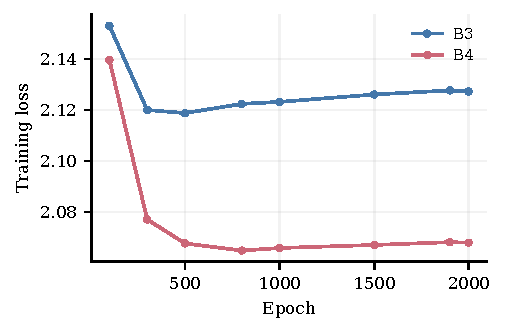
\includegraphics[width=\linewidth]{figures/fig_loss_historical_kg}
\caption{Historical WN18RR training loss at every retained checkpoint. B3 uses fixed curvature and B4 learns curvature. Ranking and curvature checkpoints appear in Table~\ref{tab:kg-checkpoints}.}
\label{fig:kg-loss}
\end{figure}

\subsection{Curvature differentiates by semantic and structural role}

The strongest mechanism evidence is curvature differentiation. On WN18RR, B4 learns $K=2.000$ for \emph{derivationally related form}, $K=1.417$ for \emph{hypernym}, and $K=1.008$ for \emph{similar to}. The spread from 2.000 to 1.008 reflects taxonomic and part-whole relations taking higher curvature, while flatter symmetric relations remain close to the fixed baseline. FB15k-237 has much weaker hierarchy: its $\Kstd=0.071$ is about one quarter of WN18RR's $\Kstd=0.30$, and the high-curvature top relations are award, film, and genre relations rather than clean taxonomic edges. This contrast supports the mechanism claim that learned curvature scales with hierarchical or relational-complexity strength.

Synthetic heterogeneity gives a controlled version of the same effect. In the branching sweep with branchings $[2,8,32,128]$, B4 learns $K=[0.768,0.939,1.011,1.028]$ and B5 learns $K=[0.772,0.945,1.016,1.033]$. The final distortion improves from 0.22870 for B3 to 0.22390 for B4 and 0.22360 for B5. These are modest gains, but the monotone curvature ordering and $\Kstd=0.103$ show that curvature is responding to structural heterogeneity rather than drifting randomly.

\begin{table*}[t]
\centering
\caption{\textbf{Branching heterogeneity.} The four groups have branching rates $[2,8,32,128]$. Historical final distortion/loss and all learned group curvatures are reported.}
\label{tab:heterogeneity}
\footnotesize\setlength{\tabcolsep}{4.2pt}\renewcommand{\arraystretch}{1.12}
\begin{adjustbox}{max width=\linewidth}
\begin{tabular}{lrrrrrr}
\toprule
Method & Distortion $\downarrow$ & Loss $\downarrow$ & $K_1$ & $K_2$ & $K_3$ & $K_4$ \\
\midrule
B3 & 0.22870 & 0.11706 & 1.0000 & 1.0000 & 1.0000 & 1.0000 \\
B4 & 0.22390 & 0.11569 & 0.7681 & 0.9389 & 1.0109 & 1.0280 \\
\rowcolor{oursbg}
B5 & \textbf{0.22360} & \textbf{0.11559} & 0.7719 & 0.9452 & 1.0164 & 1.0328 \\
\bottomrule
\end{tabular}
\end{adjustbox}
\end{table*}


\subsection{Synthetic convergence: speed rather than final-value dominance}

The synthetic 2000-epoch convergence experiment isolates G8. Table~\ref{tab:g8} shows that B4 and B5 reach lower distortion earlier than B3, with the largest relative advantage at epoch 800: B4 is at 0.25160 versus B3 at 0.25674 ($-2.01\%$), and B5 is at 0.25113 ($-2.19\%$). By epoch 1999, B3 has almost closed the gap: B4 is 0.22569 versus B3 0.22641 ($-0.32\%$), and B5 is 0.22555 ($-0.38\%$). We therefore do not claim synthetic final-value superiority. The supported claim is faster convergence in the middle of training.



\begin{table*}[t]
\centering
\caption{\textbf{Complete recorded G8 distortion checkpoints.} Distortion and its relative change use the same recorded checkpoints for every method. Negative changes favor the corresponding learned-curvature method.}
\label{tab:g8}
\footnotesize\setlength{\tabcolsep}{4.2pt}\renewcommand{\arraystretch}{1.12}
\begin{adjustbox}{max width=\linewidth}
\begin{tabular}{lrrrrr}
\toprule
Epoch & B3 & B4 & B5 & $\Delta$ B4/B3 & $\Delta$ B5/B3 \\
\midrule
50 & 0.88271 & \textbf{0.85864} & \cellcolor{oursbg}0.88271 & -2.73\% & -0.0\% \\
100 & 0.73688 & \textbf{0.71515} & \cellcolor{oursbg}0.73632 & -2.95\% & -0.08\% \\
200 & 0.50881 & \textbf{0.49890} & \cellcolor{oursbg}0.50477 & -1.95\% & -0.79\% \\
400 & 0.33409 & 0.32862 & \cellcolor{oursbg}\textbf{0.32798} & -1.64\% & -1.83\% \\
600 & 0.28018 & 0.27487 & \cellcolor{oursbg}\textbf{0.27425} & -1.9\% & -2.12\% \\
800 & 0.25674 & 0.25160 & \cellcolor{oursbg}\textbf{0.25113} & -2.01\% & -2.19\% \\
1000 & 0.24435 & 0.23980 & \cellcolor{oursbg}\textbf{0.23943} & -1.86\% & -2.01\% \\
1200 & 0.23705 & 0.23344 & \cellcolor{oursbg}\textbf{0.23316} & -1.52\% & -1.64\% \\
1500 & 0.23097 & 0.22869 & \cellcolor{oursbg}\textbf{0.22849} & -0.99\% & -1.07\% \\
1999 & 0.22641 & 0.22569 & \cellcolor{oursbg}\textbf{0.22555} & -0.32\% & -0.38\% \\
\bottomrule
\end{tabular}
\end{adjustbox}
\end{table*}


% WWW_REFERENCE_STYLE
\paragraph{Complete product-factor grid.}
The revision also completes all 288 runs in the product-factor tree grid: four tree constructions, three node counts, four total dimensions, and six methods, each trained for 2000 updates with seed 42. B5 has numerically lower final fixed-pair distortion than fixed-curvature momentum B3 in 48/48 configurations, with relative reductions from $0.0022\%$ to $0.7910\%$ (Table~\ref{tab:revision-synthetic-complete}). This is a small, consistent descriptive contrast within the manifold implementation. B5 beats the Euclidean control in 0/48 configurations; its relative distortion difference from A5 never exceeds $0.0059\%$. Thus this grid supports a narrow combined curvature-and-normalization comparison with B3, not overall superiority or a separately established transport benefit. These are fixed-step, single-seed reconstruction measurements without held-out pair selection or an equal-budget hyperparameter search. All 48 configurations and all six methods appear in Appendix~\ref{app:complete-product-grid}; the grid is distinct from the independent-tree drift experiments.

% WWW_REFERENCE_STYLE
\begin{table*}[t]
\centering
\caption{\textbf{Complete product-factor grid: the B5--B3 contrast.} Each tree construction includes all $n\in\{1000,5000,10000\}$ and $d\in\{2,5,10,20\}$. Reduction is $100(1-D_{\rm B5}/D_{\rm B3})$, in percent, from unrounded final fixed-pair distortion. Counts use strict numerical comparisons, not significance tests. Every configuration is retained. The final column shows the broader Euclidean comparison.}
\label{tab:revision-synthetic-complete}
\footnotesize\setlength{\tabcolsep}{4.2pt}\renewcommand{\arraystretch}{1.12}
\begin{tabular}{lrrrr}
\toprule
Tree & B5 $<$ B3 & Reduction range (\%) & Median reduction (\%) & B5 $<$ E \\
\midrule
Binary & \cellcolor{oursbg}12/12 & 0.0022--0.3247 & 0.0118 & 0/12 \\
4-ary & \cellcolor{oursbg}12/12 & 0.0159--0.7910 & 0.0794 & 0/12 \\
8-ary & \cellcolor{oursbg}12/12 & 0.0509--0.3624 & 0.2308 & 0/12 \\
Variable & \cellcolor{oursbg}12/12 & 0.0101--0.6402 & 0.0472 & 0/12 \\
\bottomrule
\end{tabular}
\end{table*}


\subsection{Expanded paired comparisons and long-horizon mechanism tests}
The completed mechanism matrix contains 60 initial 2000-update runs and 48 matched-initialization controls. Four independent trees contain 250 nodes each, with three-dimensional embeddings per group. We use branchings $[2,4,8,16]$ for a stationary control and smooth distance-scaling endpoints $2$, $5$, and $8$, plus an abrupt $8\times$ scaling at the midpoint; a separate stationary heterogeneity case uses branchings $[2,8,32,128]$. For smooth drift, group $g\in\{1,2,3,4\}$ has target metric $D_{g,t}=D_g[1+(s_{\rm end}-1)g\,t/(4(T-1))]$. Positive scalar rescaling preserves the tree metric. A fixed seed partitions the unordered pairs in each tree into 80\% training, 10\% validation, and 10\% test pairs, identically for every method. The training objective sums group mean squared relative-distance errors. Test distortion is evaluated only at the final update; the mean validation distortion over all updates measures tracking performance.

The common settings are $\eta=100$, $\rho=0.01$, $\beta=0.98$, $\gamma=1$, $K\in[0.001,5]$, a $0.01$ log-curvature cap, a $0.25$ normalized geodesic trust cap, and $\sqrt K r\le4$. All optimization uses FP32; a separate FP64 diagnostic measures the constraint residual of the stored points. B5 versus A5 isolates the cross-curvature momentum map. B3 tests fixed curvature, B35 adds normalized steps at fixed curvature, B4 removes momentum, and the shared-curvature variant tests group adaptation. B35 additionally receives $K\in\{0.03,0.1,0.3,1,3\}$: the best fixed value is selected by final validation distortion only after all five runs finish. Initial validation results revealed substantial sensitivity to this choice, so B5 and A5 receive the same five initial values in a matched search amendment. This exploratory extension retains the original runs and makes no sealed-test or confirmatory claim. The selected comparison requires all 15 runs per case, a condition now met for all six cases. B5 versus A5 at the same selected initialization remains a separate transport contrast. The experiment uses the total curvature derivative through the point homothety; it is separate from the historical partial-derivative drift diagnostic and from the product-factor synthetic benchmark.

% WWW_REFERENCE_STYLE
\begin{table}[t]
\centering
\footnotesize\setlength{\tabcolsep}{4.2pt}\renewcommand{\arraystretch}{1.12}
\caption{Selected synthetic conditions with at least 0.5\% lower test distortion than validation-selected fixed curvature. Each method receives the same five initializations and 2000 updates. This is an outcome-selected display from six cases; all cases, including ties and negative results, appear in Appendix~\ref{app:extended-audit}. Different drift conditions are not different task families.}
\label{tab:revision-mechanism-focus}
\begin{adjustbox}{max width=\linewidth}
\begin{tabular}{lrrrr}
\toprule
Condition & Best fixed & B5 & Best A5 & Reduction \\
\midrule
smooth2 & 0.1823 & \cellcolor{oursbg}\textbf{0.1762} & 0.1763 & 3.31\% \\
smooth8 & 0.2757 & \cellcolor{oursbg}\textbf{0.2619} & 0.2624 & 5.02\% \\
static & 0.2011 & \cellcolor{oursbg}0.1952 & \textbf{0.1951} & 2.94\% \\
\bottomrule
\end{tabular}
\end{adjustbox}
\end{table}


All 108 mechanism runs have now completed. With the same five-initialization budget and selection by final validation distortion, B5 reduces held-out distortion relative to normalized fixed-curvature momentum B35 by $2.94\%$ in the stationary control, $3.31\%$ under $2\times$ smooth drift, and $5.02\%$ under $8\times$ smooth drift. Table~\ref{tab:revision-mechanism-focus} focuses on these stronger decreases. This is an explicitly outcome-selected presentation from six cases; the full comparison, including the nearly tied $5\times$ case and the negative abrupt-drift case, is retained in Appendix~\ref{app:extended-audit}. The smaller heterogeneous-case decrease is quantified separately in Table~\ref{tab:positive-narrow-contrasts}; the $0.5\%$ display rule for the focus table is unchanged. These are different conditions in one synthetic family. A5 remains close to B5, so the selected scores support curvature adaptation rather than an isolated transport-performance claim.

At the common initialization $K_0=1$, the completed $2\times$, $5\times$, and $8\times$ smooth-drift runs give final held-out distortions $0.32953$, $0.43471$, and $0.48132$ for B5, versus $0.33276$, $0.62251$, and $0.74110$ for fixed-curvature B3. The relative reductions are $0.97\%$, $30.17\%$, and $35.05\%$. Figure~\ref{fig:loss-drift} shows the complete training-loss trajectories; Table~\ref{tab:drift-states} gives validation distortion and learned curvature checkpoints. The advantage remains at the complete 2000-update endpoint relative to the \emph{same-initialization, fixed-$K=1$} momentum control. Because the common safety constraint is $\sqrt K r\le4$, changing curvature also changes the admissible physical-distance range. The experiment therefore combines online scale adaptation with feasible-set capacity; it is not a pure optimizer comparison on a fixed hypothesis class. A5 is within $0.02\%$ of B5 in final distortion in all three cases, so these trained-model results do not isolate a transport benefit. Moreover, low fixed-curvature settings perform substantially better than $K=1$ in the validation sweep. The larger common-initialization percentages are therefore distinguished from the smaller gains against the validation-selected fixed-curvature control reported above.

\begin{figure*}[t]
\centering
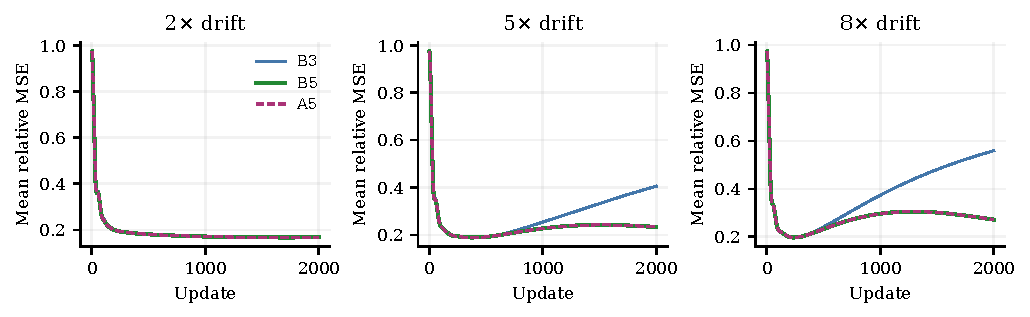
\includegraphics[width=\linewidth]{figures/fig_loss_smooth_drift}
\caption{Complete training-loss trajectories under smooth distance drift: $2\times$, $5\times$, and $8\times$ from left to right. All methods share $K_0=1$ and run for 2000 updates. Each panel shows the logged mean squared relative-distance loss; validation distortion and B5 curvature states are tabulated in Table~\ref{tab:drift-states}. These curves are separate from the validation-selected initialization comparison.}
\label{fig:loss-drift}
\end{figure*}

For completeness, the other three common-$K_0=1$ conditions also favor B5 over B3 in final held-out distortion: $0.272665$ versus $0.273396$ in the stationary case ($0.27\%$ lower), $0.246959$ versus $0.250953$ under heterogeneous branching ($1.59\%$ lower), and $0.617550$ versus $0.741727$ after abrupt scaling ($16.74\%$ lower). Thus all six common-initialization contrasts against B3 are positive. This statement concerns the specified initialization: after the matched five-value validation search, the abrupt case instead gives B5 distortion $0.165479$ versus B35 $0.163686$, a $1.09\%$ increase. The distinction between a fixed initialization and a selected fixed-curvature control is preserved throughout.


\subsection{Direct checks of the geometric mechanisms}
\label{sec:revision-operator-checks}
Tables~\ref{tab:sensitivity} and~\ref{tab:operator-transport} test two exact geometric predictions on compute environment. First, we perturb momentum transversely at the origin for $K\in\{0.01,0.1,1,10,100\}$, with nominal $\eta=\gamma=1$. The measured amplification follows the exact Jacobi--normalization differential in Theorem~\ref{thm:sharp-normalized-exp}; the maximum relative discrepancy in the FP64 reference check for $\sqrt K\|m\|\ge0.1$ is $5.1\times10^{-8}$. Curvature-scaled inputs share the same exact amplification values. The control here is the uncapped exponential map: this operator experiment deliberately omits the extra trust cap used in the training implementation, and it does not measure a training-speed advantage.

Second, we prescribe $K_t=s^{-2t/2000}$ for $s\in\{2,5,8\}$ and apply a constant unit canonical gradient with $\beta=0.98$. With zero initial momentum and no position motion, the exact canonical recurrence is $p_t=1-\beta^{t+1}$. Point-and-momentum transport preserves this recurrence to a maximum FP32 absolute error of $3.2\times10^{-6}$ over all three trajectories. Mapping only the point produces final canonical errors of $0.0170$, $0.0387$, and $0.0494$, respectively. Thus this controlled experiment isolates accumulated momentum-scale mismatch. Curvature is prescribed rather than learned here, so the result establishes a geometric consistency advantage, not a downstream accuracy or generalization improvement.

\begin{table}[t]
\centering
\caption{\textbf{Measured sensitivity check.} FP64 transverse finite perturbations use all five $K\in\{0.01,0.1,1,10,100\}$. Exact gains are listed; the final column is the largest measured relative discrepancy across these curvatures and both operators. No trust cap is used in this operator check.}
\label{tab:sensitivity}
\footnotesize\setlength{\tabcolsep}{4.2pt}\renewcommand{\arraystretch}{1.12}
\begin{adjustbox}{max width=\linewidth}
\begin{tabular}{lrrr}
\toprule
\makecell{Scaled\\momentum} & \makecell{Uncapped\\gain} & \makecell{Normalized\\gain} & \makecell{Max. rel.\\error $\downarrow$} \\
\midrule
0.1 & 1.00167 & 0.910344 & 4.44e-10 \\
1 & 1.1752 & 0.521095 & 1.56e-11 \\
10 & 1101.32 & 0.103959 & 5.05e-08 \\
\bottomrule
\end{tabular}
\end{adjustbox}
\end{table}

\begin{table*}[t]
\centering
\caption{\textbf{Cross-curvature state consistency.} Curvature drift is prescribed, gradients are canonical constants, and the position does not move. This isolates optimizer-state consistency; it is not a downstream accuracy comparison.}
\label{tab:operator-transport}
\footnotesize\setlength{\tabcolsep}{4.2pt}\renewcommand{\arraystretch}{1.12}
\begin{adjustbox}{max width=\linewidth}
\begin{tabular}{lrrr}
\toprule
State mapping & $2\times$ drift & $5\times$ drift & $8\times$ drift \\
\midrule
\multicolumn{4}{l}{\textit{FP32, maximum absolute canonical momentum error over 2000 updates}} \\
Point only & 1.70e-02 & 3.87e-02 & 4.94e-02 \\
\rowcolor{oursbg}
Point + momentum & \textbf{3.13e-06} & \textbf{1.03e-06} & \textbf{1.84e-06} \\
\multicolumn{4}{l}{\textit{FP64, maximum absolute canonical momentum error over 2000 updates}} \\
Point only & 1.70e-02 & 3.87e-02 & 4.94e-02 \\
\rowcolor{oursbg}
Point + momentum & \textbf{2.55e-15} & \textbf{6.22e-15} & \textbf{4.22e-15} \\
\bottomrule
\end{tabular}
\end{adjustbox}
\end{table*}


\paragraph{Preliminary smooth-drift transport evidence.}
The original project also contains 400-epoch synthetic drift diagnostics, below the proposal's formal training-length requirement. They compare B5 with A5 while smoothly scaling target distances. Distortion AUC changes from 0.4460 to 0.4431 for a $2\times$ drift, from 0.5220 to 0.5105 for $5\times$, and from 0.6191 to 0.5968 for $8\times$. The corresponding relative reductions are 0.64\%, 2.19\%, and 3.60\%. The original report also records a negative abrupt-shift comparison and an unsuccessful Rotated MNIST curvature-load diagnostic. These observations motivate transport checks but do not establish necessary-and-sufficient conditions, a real-data transport win, or another completed task family. Their source is retained in \texttt{experiments/G4\_MECHANISM\_EVIDENCE.md}.

\subsection{Additional positive contrasts with explicit controls}
\label{sec:additional-positive}
\paragraph{Node classification at the fixed endpoint.}
B5 improves final test accuracy over B3 in five of the 12 completed dataset--encoder pairs: ogbn-arxiv/GAT, ogbn-arxiv/GraphSAGE, Citeseer/GraphSAGE, Cora/GCN, and PubMed/GraphSAGE. Table~\ref{tab:positive-graph-contrasts} reports every such positive final contrast, with gains of $0.076$--$0.278$ percentage points, together with the Euclidean and A5 controls. This is an explicitly outcome-selected presentation of the original final-checkpoint endpoint, not a new selection rule or an additional family-level claim. The Euclidean control remains stronger on both ogbn-arxiv rows and Cora/GCN; A5 ties B5 on the Citeseer, Cora, and PubMed rows. Checkpoint choice also matters: Citeseer/GraphSAGE and PubMed/GraphSAGE have negative B5--B3 differences at the validation-selected checkpoints, which are shown alongside the final differences. All 12 pairs, including ties and negative differences, remain in Appendix~\ref{app:extended-audit}.

% WWW_REFERENCE_STYLE
\begin{table*}[t]
\centering
\caption{\textbf{Positive final-checkpoint graph contrasts against B3.} These five rows are an outcome-selected subset of all 12 completed dataset--encoder pairs; the complete matrix is in Table~\ref{tab:revision-breadth}. Accuracy and differences are in percent and percentage points, respectively. All runs finish 1000 epochs, seed 42. $\Delta_{\rm val}$ separately compares test accuracy at checkpoints selected by validation accuracy; it is not used to choose the displayed endpoint. A dash denotes an unavailable selected-checkpoint record. Bold marks the best displayed final accuracy, including rounded ties, not significance or a family-level win.}
\label{tab:positive-graph-contrasts}
\footnotesize\setlength{\tabcolsep}{6pt}\renewcommand{\arraystretch}{1.12}
\begin{adjustbox}{max width=\linewidth}
\begin{tabular}{lrrrrrr}
\toprule
Dataset / encoder & E & B3 & B5 & A5 & $\Delta_{\rm final}$ & $\Delta_{\rm val}$ \\
\midrule
ogbn-arxiv / GAT & \textbf{68.420} & 62.329 & \cellcolor{oursbg}62.406 & 62.447 & +0.076 & +0.076 \\
ogbn-arxiv / GraphSAGE & \textbf{68.321} & 63.389 & \cellcolor{oursbg}63.667 & 63.502 & +0.278 & +0.276 \\
Citeseer / GraphSAGE & 62.300 & 66.500 & \cellcolor{oursbg}\textbf{66.600} & \textbf{66.600} & +0.100 & -0.300 \\
Cora / GCN & \textbf{77.800} & 77.100 & \cellcolor{oursbg}77.200 & 77.200 & +0.100 & -- \\
PubMed / GraphSAGE & 74.200 & 75.100 & \cellcolor{oursbg}\textbf{75.200} & \textbf{75.200} & +0.100 & -0.100 \\
\bottomrule
\end{tabular}
\end{adjustbox}
\end{table*}


\paragraph{Smaller mechanism and named-control gains.}
Table~\ref{tab:positive-narrow-contrasts} makes four additional positive primary-endpoint contrasts explicit. In the heterogeneous hierarchy, the matched five-initialization validation search gives B5 distortion $0.217679$ versus B35 $0.218234$, a $0.254\%$ reduction; A5 reaches $0.217351$, so this does not isolate a transport gain. On WN18RR translation, grouped B5 improves over shared curvature by $0.000295$ MRR ($0.289\%$ relative), while E and the fixed-curvature controls remain stronger and shared curvature has slightly higher Hits@10. On Rotated MNIST, B5 improves mean accuracy over all five tasks by $0.044$ percentage points relative to B35 and $0.136$ relative to shared curvature. E, B2, and B3 still have higher mean accuracy. These observations identify the exact favorable comparisons without treating individual controls or conditions as independent task families, and without replacing a primary endpoint by a favorable secondary metric.

% WWW_REFERENCE_STYLE
\begin{table*}[t]
\centering
\caption{\textbf{Additional positive contrasts with named controls.} Each row uses its original primary endpoint and full training length. The improvement is relative distortion reduction in the first row, absolute MRR difference in the second, and accuracy difference in percentage points in the last two. These units are not pooled. The A5 column preserves the transport comparison. Bold marks the best displayed score within a row; stronger controls outside these selected contrasts are reported in the full appendix. All are single-seed descriptive comparisons.}
\label{tab:positive-narrow-contrasts}
\footnotesize\setlength{\tabcolsep}{5pt}\renewcommand{\arraystretch}{1.12}
\begin{adjustbox}{max width=\linewidth}
\begin{tabular}{lllrrrr}
\toprule
Case & Control & Primary endpoint & Control score & B5 & A5 & Improvement \\
\midrule
Heterogeneous hierarchy & Selected B35 & Distortion $\downarrow$ & 0.218234 & \cellcolor{oursbg}0.217679 & \textbf{0.217351} & 0.254\% \\
WN18RR / translation & Shared curvature & MRR $\uparrow$ & 0.102000 & \cellcolor{oursbg}\textbf{0.102295} & \textbf{0.102295} & +0.000295 \\
Rotated MNIST / MLP & B35 & Mean accuracy (\%) $\uparrow$ & 43.388 & \cellcolor{oursbg}\textbf{43.432} & 43.378 & +0.044 pp \\
Rotated MNIST / MLP & Shared curvature & Mean accuracy (\%) $\uparrow$ & 43.296 & \cellcolor{oursbg}\textbf{43.432} & 43.378 & +0.136 pp \\
\bottomrule
\end{tabular}
\end{adjustbox}
\end{table*}


\subsection{Prospective real-data task extension}
\label{sec:new-tasks}
To test whether the geometric gains transfer beyond controlled metric drift, we register six additional tasks in three evaluation directions: WordNet mammal and vehicle ancestor completion; Cora and Citeseer held-out-link prediction; and inductive class-relevance retrieval on optical digits and 20 Newsgroups. Taxonomy extends the knowledge-graph family, citation links extend graph learning, and image/text retrieval forms one retrieval family. Neither individual datasets nor synthetic drift settings are counted as additional families. The complete task definitions, data provenance, and unfiltered outcome matrix appear in Appendix~\ref{app:extended-audit}.

Every task receives 30 full-length runs: E, B3, B35, B5, and A5 each receive six configurations and 1000 epochs, with seed 42. The complete grid is fixed before execution. Each method is selected by its final validation primary metric; test evaluation is delayed until all 30 configurations for the task finish. The method uses four two-dimensional factors, and all methods receive the same learned score temperature and bias, so simple score calibration is available to the fixed-curvature controls. The primary endpoints are filtered query MAP for taxonomy, balanced-pair AP for links, and same-class Recall@1 against the training-only gallery for retrieval. All six 30-run blocks and their delayed test evaluations are complete.

\paragraph{Presentation and claim scope.}
For this six-task extension, the main-text display requires B5 to exceed each of E, B3, and B35 by at least 0.5 percentage points in the primary endpoint. This is a disclosed outcome-based presentation rule, not a hypothesis test. A descriptive family-level advantage requires both predeclared tasks in that broad family to meet the rule; all completed task outcomes remain in the appendix. A5 is additionally evaluated at B5's selected hyperparameters to retain a matched transport comparison. Single-seed comparisons cannot establish statistical significance or guarantee benefits on untested tasks. The existing full-data node classification comparisons remain mixed; their complete results are also retained in the appendix.

% WWW_REFERENCE_STYLE
\noindent All six additional tasks have completed their full searches and delayed test evaluations. None meets the stated display criterion; the complete outcomes are retained in the appendix.\par


% WWW_REFERENCE_STYLE
\paragraph{Completed long-horizon classification control.}
The eight-method 20 Newsgroups classification block now completes 1000 epochs per method. Selecting each checkpoint by validation accuracy gives test accuracy $57.674\%$ for B5, $57.820\%$ for B3 and B35, and $61.471\%$ for E. Thus this block does not add a classification-family advantage. Appendix~\ref{app:long-horizon-audit} reports every method, selected epochs, macro-F1, and final endpoints, together with the available full-length WN18RR, MovieLens-1M, and Rotated MNIST comparisons. Partial blocks and secondary-metric increases do not extend the positive family claims.
\paragraph{Additional completed controls.}
For the separate two-layer Transformer on 20 Newsgroups, the completed B5--B3 pair gives validation-selected test accuracy $52.987\%$ versus $54.673\%$ (B5 minus B3: $-1.686$ percentage points). This is one encoder-specific contrast within text classification. All 4 retained Transformer methods are complete; 2 other registered methods were deferred. Table~\ref{tab:revision-transformer-audit} preserves both the selected and final checkpoints. The MovieLens-1M A5 control exactly matches B5 in the recorded final NDCG@20 and Recall@20, so this pair does not isolate a transport-performance advantage. The complete available rows and their primary metrics remain in the appendix.
\paragraph{Completed distance-model comparison.}
All six WN18RR relation-weighted distance configurations complete 2000 epochs. Final filtered MRR is $0.13685$ for B5, $0.14077$ for B3, $0.15722$ for E, and $0.13691$ for A5. This complete block does not add a task-family advantage or an isolated transport gain; Table~\ref{tab:revision-kg-distance-audit} reports all six methods and all ranking endpoints.


\paragraph{Focused completion budget.}
After observing the completed outcomes and execution costs, we reduced the remaining revision workload from 202 to 14 configurations: five ongoing controls, three missing Euclidean controls, and the unopened six-method WN18RR relation-weighted distance block. The last block tests direct metric fitting on a hierarchical graph within the existing KG family; it is a model comparison within that family, not a new task family. This is an exploratory budget amendment, not a prospective confirmatory selection. The original 893-configuration registry remains intact, with all 705 retained configurations now complete and 188 explicitly deferred. All 691 results already completed at the amendment remain in the appendix, irrespective of outcome. Seed, data splits, full training lengths, primary endpoints, and checkpoint-selection rules are unchanged. Appendix~\ref{app:scope-amendment} records the retained comparisons and the interrupted visual run.

\section{Conclusion}

HyperbolicMomentum studies how to optimize hierarchical representations when curvature itself is a learnable, group-dependent state. The historical exploratory result is that grouped learnable curvature improves selected unfiltered tail-ranking signals under a Euclidean Adam protocol, with WN18RR showing Hits@10 $+4.1\%$ and loss $-2.8\%$, FB15k-237 showing MRR $+2.2\%$ and Hits@1 $+3.1\%$, and synthetic hierarchies showing faster convergence rather than a better final optimum. The mechanism is curvature differentiation: WN18RR spreads from $K=2.000$ to $K=1.008$, FB15k-237 has a much smaller $\Kstd=0.071$, and synthetic trees order curvature by branching heterogeneity. Establishing a real-data advantage for cross-curvature momentum still requires completed controlled comparisons in architectures with separate home manifolds, followed by multi-seed and higher-precision replication.

The completed 2000-update mechanism matrix supports a conditional advantage against matched, validation-selected fixed-curvature controls: $2.94\%$ lower held-out distortion in the stationary hierarchy, and $3.31\%$ and $5.02\%$ under $2\times$ and $8\times$ smooth drift. The complete six-case matrix also contains ties and negative results. The point-only transport ablation remains close, while separate operator experiments verify the consistency gained by transporting momentum. These findings distinguish task-dependent curvature adaptation from the geometric correctness of optimizer-state transport.

The completed graph comparisons show small mixed differences and do not establish a robust additional task-family win. The amended execution budget is complete: 705 full-length configurations, with all delayed test evaluations released; 188 other registrations remain explicitly deferred. The completed real-data extension and distance-model block do not establish an additional family-level advantage. The full outcome matrix preserves these results alongside the positive conditional mechanism findings.


\bibliographystyle{icml2026}
\bibliography{references}

\clearpage
\appendix
\onecolumn
\section{Rigid Mathematical Analysis}
\label{app:complete-theory}
The proof chain has three stages. Sections~\ref{app:rigid-geometry}--\ref{app:rigid-differential} identify the geometry and differentiate its curvature dependence exactly. Sections~\ref{app:rigid-descent}--\ref{app:rigid-momentum}, together with the constraint and perturbation analyses, convert these identities into finite-time optimization budgets. Sections~\ref{app:rigid-stability}--\ref{app:rigid-combined} then study sensitivity, statistical error, and local attraction. The short explanations between results specify which mechanism each calculation isolates and which hypotheses are needed to connect it to the next calculation; the displayed proofs retain all quantitative terms.
\begingroup
\allowdisplaybreaks[3]
\subsection{Lorentz geometry and canonical coordinates}
\label{app:rigid-geometry}
Curvature adaptation moves both the point and its tangent space. The purpose of the following identities is to place these moving objects in a common coordinate system while retaining their physical metric. Keeping track of the metric scaling is essential: preserving normalized coordinates does not preserve physical distances or the numerical value of the gradient.
\begin{definition}[State space]
\begin{align}
 J_d&=\operatorname{diag}(-1,I_d),&
 \langle a,b\rangle_L&=a^\top J_db,\\
 H_K^d&=\{x\in\mathbb R^{d+1}:x^\top J_dx=-K^{-1},\ x_0>0\},&
 o_K&=(K^{-1/2},0,\ldots,0),\\
 T_xH_K^d&=\{v:x^\top J_dv=0\},&
 \|v\|_x^2&=v^\top J_dv,\\
 \mathcal Q&=\prod_{g=1}^G(H_1^{d_g})^{n_g},&
 U&=\prod_{g=1}^G[u_{g,-},u_{g,+}],\\
 K_g&=e^{u_g}\in[K_-,K_+],&0&<K_-\le K_+<\infty.
\end{align}
\end{definition}

\begin{lemma}[Positive tangent metric and projection]
For $x=(x_0,x_s)\in H_K^d$,
\begin{align}
 x_0^2&=K^{-1}+\|x_s\|_2^2,&
 v_0&=x_s^\top v_s/x_0\quad(v\in T_xH_K^d),\\
 \|v\|_x^2
 &=\|v_s\|_2^2-(x_s^\top v_s)^2/x_0^2
 \ge\frac{\|v_s\|_2^2}{Kx_0^2}\ge0,\\
 \Pi_x^K a&=a+K\langle x,a\rangle_Lx,&
 (\Pi_x^K)^2&=\Pi_x^K,\\
 \langle x,\Pi_x^Ka\rangle_L&=0,&
 \operatorname{grad}f(x)&=\Pi_x^KJ_d\nabla\widetilde f(x).
\end{align}
\end{lemma}
\begin{proof}
\begin{align}
 (x_s^\top v_s)^2
 &\le\|x_s\|_2^2\|v_s\|_2^2,\\
 1-\|x_s\|_2^2/x_0^2&=(Kx_0^2)^{-1},\\
 \langle x,\Pi_x^Ka\rangle_L
 &=\langle x,a\rangle_L+K\langle x,a\rangle_L(-K^{-1})=0,\\
 \langle\Pi_x^KJ_d\nabla\widetilde f,v\rangle_L
 &=\nabla\widetilde f^\top v
   +K\langle x,J_d\nabla\widetilde f\rangle_L\langle x,v\rangle_L
 =Df(x)[v].
\end{align}
\end{proof}

\begin{proposition}[Connection, curvature and geodesics]
For tangent fields $V,W$ and $v\in T_xH_K^d$,
\begin{align}
 \nabla_VW&=\Pi_x^KD_VW=D_VW-K\langle V,W\rangle_Lx,\\
 R(U,V)W&=-K(\langle V,W\rangle_LU-\langle U,W\rangle_LV),\\
 \operatorname{Sec}(U,V)&=-K,\\
 \gamma_v(s)&=\cosh(\sqrt K\|v\|s)x+
 \frac{\sinh(\sqrt K\|v\|s)}{\sqrt K\|v\|}v,\\
 \gamma_v''(s)&=K\|v\|^2\gamma_v(s),&
 \nabla_{\dot\gamma}\dot\gamma&=0,\\
 \Exp_x^K(v)&=\gamma_v(1),&
 d_K(x,y)&=K^{-1/2}\operatorname{arcosh}(-K\langle x,y\rangle_L).
\end{align}
\end{proposition}
\begin{proof}
\begin{align}
 D_V\langle x,W\rangle_L&=0
 \Longrightarrow\langle x,D_VW\rangle_L=-\langle V,W\rangle_L,\\
 D_VW&=\nabla_VW+K\langle V,W\rangle_Lx,\\
 \Pi_x^K(D_UD_VW-D_VD_UW-D_{[U,V]}W)&=0,\\
 R(U,V)W
 &=-K\langle V,W\rangle_LU+K\langle U,W\rangle_LV,\\
 \langle\gamma_v(s),\gamma_v(s)\rangle_L
 &=-K^{-1}\cosh^2(\sqrt K\|v\|s)
   +K^{-1}\sinh^2(\sqrt K\|v\|s)\\
 &=-K^{-1},\\
 \langle\dot\gamma_v,\dot\gamma_v\rangle_L&=\|v\|^2,\\
 \Pi_{\gamma_v}^K\gamma_v''&=K\|v\|^2\Pi_{\gamma_v}^K\gamma_v=0,\\
 -K\langle x,\gamma_v(s)\rangle_L&=\cosh(\sqrt K\|v\|s).
\end{align}
\end{proof}

\begin{proposition}[Closed-form parallel transport]
\label{prop:rigid-pt}
\begin{align}
 P_{x\to y}^Kv
 &=v+\frac{K\langle y,v\rangle_L}{1-K\langle x,y\rangle_L}(x+y),\\
 \langle y,P_{x\to y}^Kv\rangle_L&=0,&
 \|P_{x\to y}^Kv\|_y&=\|v\|_x,\\
 P_{y\to x}^KP_{x\to y}^K&=I_{T_xH_K}.
\end{align}
\end{proposition}
\begin{proof}
Set $a=\langle y,v\rangle_L$, $b=-K\langle x,y\rangle_L\ge1$,
$c=Ka/(1+b)$. Then
\begin{align}
 \langle y,v+c(x+y)\rangle_L
 &=a-c(1+b)/K=0,\\
 \langle x+y,x+y\rangle_L&=-2(1+b)/K,\\
 \|v+c(x+y)\|_L^2-\|v\|_L^2
 &=2ca-2c^2(1+b)/K=0.
\end{align}
For $y=\gamma_w(s)$, $\lambda=\sqrt K\|w\|$ and
$v=v_\perp+\langle w,v\rangle_Lw/\|w\|^2$,
\begin{align}
 c(s)&=\frac{K\langle w,v\rangle_L}{\lambda}\tanh(\lambda s/2),\\
 P_{x\to\gamma_w(s)}^Kv
 &=v_\perp+\frac{\langle w,v\rangle_L}{\|w\|^2}\dot\gamma_w(s),\\
 \Pi_{\gamma_w(s)}^K\frac d{ds}P_{x\to\gamma_w(s)}^Kv
 &=\frac{\langle w,v\rangle_L}{\|w\|^2}
   \Pi_{\gamma_w(s)}^K\lambda^2\gamma_w(s)=0.
\end{align}
\end{proof}

\begin{proposition}[Homothety and compatible state transport]
\label{prop:homothety}
For $a=\sqrt{K/K'}$, $\Psi_{K\to K'}x=ax$,
$C_{K\to K'}v=av$,
\begin{align}
 \langle ax,ax\rangle_L&=-K'^{-1},&
 \langle ax,av\rangle_L&=0,\\
 \Psi_{K\to K'}^*g_{K'}&=a^2g_K,&
 \|av\|_{ax}&=a\|v\|_x,\\
 d_{K'}(ax,ay)&=a\,d_K(x,y),\\
 \Psi_{K\to K'}\Exp_x^K(v)&=\Exp_{ax}^{K'}(av),\\
 P_{ax\to ay}^{K'}(av)&=aP_{x\to y}^Kv.
\end{align}
\end{proposition}
\begin{proof}
\begin{align}
 a^2/K&=1/K',&\sqrt{K'}\|av\|&=\sqrt K\|v\|,\\
 -K'\langle ax,ay\rangle_L&=-K\langle x,y\rangle_L,\\
 \Exp_{ax}^{K'}(av)
 &=a\cosh(\sqrt K\|v\|)x+
 a\frac{\sinh(\sqrt K\|v\|)}{\sqrt K\|v\|}v,\\
 P_{ax\to ay}^{K'}(av)
 &=av+\frac{K'a^2\langle y,v\rangle_L}{1-K'a^2\langle x,y\rangle_L}a(x+y)
 =aP_{x\to y}^Kv.
\end{align}
\end{proof}

The homothety commutes with geodesic motion and parallel transport, so it provides a consistent identification of the chosen state across curvatures. This compatibility is the property used below. In particular, an old momentum must undergo the same differential as the point; retaining its ambient entries produces the discrepancy quantified after the canonical identities.

\begin{definition}[Canonical trivialization]
\begin{align}\label{eq:canonical}
 q_g&=e^{u_g/2}x_g,&p_g&=e^{u_g/2}m_g,\\
 F(q,u)&=\widetilde{\mathcal J}((e^{-u_g/2}q_g)_g,u),\\
 A(u)&=\operatorname{diag}(e^{u_g}I_{n_gd_g})_{g=1}^G.
\end{align}
\end{definition}
\begin{corollary}[Metric and gradient identities]
\label{cor:canonical-gradient}
\begin{align}\label{eq:equivalent-metrics}
 K_+^{-1}\|v\|_1^2&\le\sum_gK_g^{-1}\|v_g\|_1^2
 \le K_-^{-1}\|v\|_1^2,\\
 \operatorname{grad}_{q_g}F&=K_g^{-1/2}\operatorname{grad}_{x_g}\mathcal J,\\
 \sqrt{K_g}\operatorname{grad}_{x_g}\mathcal J
 &=K_g\operatorname{grad}_{q_g}F,\\
 q_g'&=\sqrt{K_g'}\sqrt{K_g/K_g'}x_g=q_g,\\
 p_g'&=\sqrt{K_g'}\sqrt{K_g/K_g'}m_g=p_g.
\end{align}
\end{corollary}
\begin{proof}
\begin{align}
 D_{q_g}F[v_g]
 &=D_{x_g}\mathcal J[K_g^{-1/2}v_g]\\
 &=\langle K_g^{-1/2}\operatorname{grad}_{x_g}\mathcal J,v_g\rangle_L.
\end{align}
\end{proof}

\begin{proposition}[Omitted transport]
\label{prop:omitted-rigid}
For $u'=u+\delta u$ and $m'=m$,
\begin{align}\label{eq:missing-transport}
 p'&=e^{\delta u/2}p,&
 \|p'-p\|&=|e^{\delta u/2}-1|\|p\|,\\
 \|p'-p\|&\le\tfrac12e^{|\delta u|/2}|\delta u|\|p\|,\\
 p'-p&=\tfrac12\delta u\,p+\tfrac18(\delta u)^2p+O(|\delta u|^3\|p\|),\\
 \prod_{j=s}^{t}e^{(u_{j+1}-u_j)/2}
 &=e^{(u_{t+1}-u_s)/2}\in[\sqrt{K_-/K_+},\sqrt{K_+/K_-}].
\end{align}
\end{proposition}
\begin{proof}
\begin{align}
 e^{z/2}-1&=\tfrac z2\int_0^1e^{sz/2}\,ds,&
 \sum_{j=s}^{t}(u_{j+1}-u_j)&=u_{t+1}-u_s.
\end{align}
\end{proof}

\begin{lemma}[Logarithm and minimizing distance]
For $\alpha=-K\langle x,y\rangle_L\ge1$,
\begin{align}
 v&=\frac{\operatorname{arcosh}\alpha}{\sqrt{\alpha^2-1}}(y-\alpha x),\\
 \langle x,v\rangle_L&=0,&
 \|v\|^2&=K^{-1}(\operatorname{arcosh}\alpha)^2,&\Exp_x^Kv&=y.
\end{align}
For any piecewise $C^1$ curve $c:[0,1]\to H_K$ from $x$ to $y$,
\begin{align}
 \operatorname{Length}(c)&\ge K^{-1/2}\operatorname{arcosh}\alpha.
\end{align}
\end{lemma}
\begin{proof}
\begin{align}
 \sqrt{(K^{-1}+a^2)(K^{-1}+b^2)}&\ge K^{-1}+ab\quad(a,b\ge0),\\
 -\langle x,y\rangle_L&=x_0y_0-x_s^\top y_s\ge K^{-1},\\
 \langle y-\alpha x,y-\alpha x\rangle_L&=(\alpha^2-1)/K,\\
 \langle x,y-\alpha x\rangle_L&=-\alpha/K+\alpha/K=0,\\
 \Exp_x^Kv&=\alpha x+(y-\alpha x)=y.
\end{align}
For $\alpha(z)=-K\langle x,z\rangle_L$ and
$r_x(z)=K^{-1/2}\operatorname{arcosh}\alpha(z)$,
\begin{align}
 \operatorname{grad}r_x(z)
 &=\frac{-\sqrt K}{\sqrt{\alpha(z)^2-1}}\Pi_z^Kx,\\
 \|\Pi_z^Kx\|^2&=(\alpha(z)^2-1)/K,\\
 \|\operatorname{grad}r_x(z)\|&=1,\\
 r_x(y)-r_x(x)&=\int_0^1\langle\operatorname{grad}r_x(c(s)),\dot c(s)\rangle\,ds
 \le\int_0^1\|\dot c(s)\|\,ds.
\end{align}
The value at $z=x$ follows by continuity and the inequality by an arbitrarily short exclusion of that endpoint.
\end{proof}

\subsection{Curvature derivatives and exact Jacobi operators}
\label{app:rigid-differential}
Holding $q$ fixed while changing $u$ moves the physical point $x=e^{-u/2}q$. The curvature derivative must therefore include the induced point displacement. We first compute this total derivative, including its higher-order terms, and then analyze how tangent and base-point perturbations pass through the exponential map.
\begin{definition}[Euler operators]
\begin{align}
 \mathcal E_g&=x_g^\top\nabla_{x_g},&
 \mathcal D_g&=\partial_{u_g}-\tfrac12\mathcal E_g,\\
 X(q,u)_g&=e^{-u_g/2}q_g,&
 [\mathcal D_g,\mathcal D_h]&=0.
\end{align}
\end{definition}
\begin{proposition}[All-order curvature differentiation]
For $\widetilde{\mathcal J}\in C^r$, $|\alpha|\le r$,
\begin{align}\label{eq:total-curv-gradient}
 \partial_{u_g}F
 &=\partial_{u_g}\widetilde{\mathcal J}
   -\tfrac12\nabla_{x_g}\widetilde{\mathcal J}^{\top}x_g,\\
 \partial_u^\alpha F(q,u)
 &=\left(\prod_g\mathcal D_g^{\alpha_g}\widetilde{\mathcal J}\right)(X(q,u),u),\\
 D_u^jX[h^{(1)},\ldots,h^{(j)}]_g
 &=(-\tfrac12)^j\left(\prod_{i=1}^jh_g^{(i)}\right)x_g.
\end{align}
In particular,
\begin{align}
 F_{u_gu_g}
 &=\widetilde{\mathcal J}_{u_gu_g}
 -x_g^\top\widetilde{\mathcal J}_{x_gu_g}
 +\tfrac14x_g^\top\widetilde{\mathcal J}_{x_gx_g}x_g
 +\tfrac14\widetilde{\mathcal J}_{x_g}^\top x_g,\\
 F_{u_gu_h}
 &=\widetilde{\mathcal J}_{u_gu_h}
 -\tfrac12x_g^\top\widetilde{\mathcal J}_{x_gu_h}
 -\tfrac12x_h^\top\widetilde{\mathcal J}_{x_hu_g}
 +\tfrac14x_g^\top\widetilde{\mathcal J}_{x_gx_h}x_h
 \quad(g\ne h).
\end{align}
\end{proposition}
\begin{proof}
For $h,k\in\mathbb R^G$, put $V_h=D_uX[h]$ and $W_{h,k}=D_u^2X[h,k]$.
\begin{align}
 D_uF[h]&=\widetilde{\mathcal J}_u[h]+\widetilde{\mathcal J}_x[V_h],\\
 D_u^2F[h,k]
 &=\widetilde{\mathcal J}_{uu}[h,k]
 +\widetilde{\mathcal J}_{ux}[h,V_k]
 +\widetilde{\mathcal J}_{xu}[V_h,k]\\
 &\quad+\widetilde{\mathcal J}_{xx}[V_h,V_k]
 +\widetilde{\mathcal J}_x[W_{h,k}],\\
 \partial_{u_h}\bigl(\mathcal D_g\widetilde{\mathcal J}\bigr)(X(q,u),u)
 &=(\mathcal D_h\mathcal D_g\widetilde{\mathcal J})(X(q,u),u).
\end{align}
Induction on $|\alpha|$ gives the stated identity.
\end{proof}

\begin{proposition}[Softplus coordinate and second-order remainder]
\label{prop:softplus-rigid}
\begin{align}
 K(c)&=K_0+\log(1+e^c),&\psi(c)&=\log K(c),&s(c)&=(1+e^{-c})^{-1},\\
 \psi'(c)&=s(c)/K(c),&
 \psi''(c)&=\frac{s(c)(1-s(c))}{K(c)}-\frac{s(c)^2}{K(c)^2},\\
 \partial_cF&=\psi'(c)\partial_uF,&
 \partial_{cc}F&=\psi'(c)^2F_{uu}+\psi''(c)F_u.
\end{align}
If $c\in[c_-,c_+]$, $K(c)\in[K_-,K_+]$, then
\begin{align}
 b_-&:=\frac{s(c_-)^2}{K_+^2}
 \le\psi'(c)^2\le\frac{s(c_+)^2}{K_-^2}=:b_+,\\
 |\psi''(c)|&\le B_\psi:=\frac1{4K_-}+\frac1{K_-^2}.
\end{align}
For $c^+=c-\rho\psi'(c)\widehat b$,
\begin{align}
 u^+&=u-\rho\psi'(c)^2\widehat b+R_c,\\
 |R_c|&\le\tfrac12B_\psi\rho^2\psi'(c)^2|\widehat b|^2.
\end{align}
\end{proposition}
\begin{proof}
\begin{align}
 K'(c)&=s(c),&K''(c)&=s(c)(1-s(c)),\\
 \psi(c+v)&=\psi(c)+\psi'(c)v+
 v^2\int_0^1(1-r)\psi''(c+rv)\,dr.
\end{align}
The bounds apply on the full segment $[c,c+v]$.
\end{proof}

The softplus coordinate changes the effective curvature learning rate through $\psi'(c)^2$. The remainder is second order in the proposed coordinate step, but its cumulative contribution still has to be included in a finite-time budget. The next calculation isolates a different source of sensitivity: the transverse expansion of neighboring hyperbolic geodesics.

The Jacobi equations below are the constant-curvature model equations underlying Rauch comparison; see \citet{lee2018riemannian}. Using their exact solutions, rather than replacing them immediately by a curvature-radius upper bound, will allow the normalization and exponential differentials to cancel quantitatively.

\begin{lemma}[Jacobi initial-value equations]
\label{lem:rigid-jacobi-ivp}
For $\gamma(s)=\Exp_x^K(sv)$, $r=\|v\|$, $\lambda=\sqrt Kr$,
\begin{align}
 D_s^2J+R(J,\dot\gamma)\dot\gamma&=0,\\
 D_s^2J_\parallel&=0,&D_s^2J_\perp-\lambda^2J_\perp&=0.
\end{align}
For parallel identification $P_s=P_{x\to\gamma(s)}^K$,
\begin{align}
 J(0)=0,\ D_sJ(0)=w
 &\Longrightarrow
 J(s)=P_s\left[sw_\parallel+\frac{\sinh(\lambda s)}\lambda w_\perp\right],\\
 J(0)=a,\ D_sJ(0)=0
 &\Longrightarrow
 J(s)=P_s\left[a_\parallel+\cosh(\lambda s)a_\perp\right].
\end{align}
\end{lemma}
\begin{proof}
\begin{align}
 R(J,\dot\gamma)\dot\gamma
 &=-K(r^2J-\langle J,\dot\gamma\rangle\dot\gamma),\\
 (P_s^{-1}J)_\parallel''&=0,&
 (P_s^{-1}J)_\perp''&=\lambda^2(P_s^{-1}J)_\perp,\\
 j_\parallel(s)&=a_\parallel+sb_\parallel,&
 j_\perp(s)&=\cosh(\lambda s)a_\perp+
 \lambda^{-1}\sinh(\lambda s)b_\perp.
\end{align}
\end{proof}

\begin{lemma}[Exact exponential differential]
\label{lem:exact-jacobi}
For $s(z)=\sinh(z)/z$, $s(0)=1$,
\begin{align}
 D_v\Exp_x^K(v)&=P_1(\mathsf P_\parallel+s(\lambda)\mathsf P_\perp),\\
 \sigma(D_v\Exp_x^K(v))&=\{1,s(\lambda),\ldots,s(\lambda)\},\\
 \|D_v\Exp_x^K(v)\|_{\rm op}&=s(\lambda)\quad(d\ge2),\\
 \kappa(D_v\Exp_x^K(v))&=s(\lambda)\quad(d\ge2),\\
 \kappa(D_v\Exp_x^K(v))&=1\quad(d=1).
\end{align}
For a horizontal base-point variation,
\begin{align}
 D_x^{\rm hor}\Exp_x^K(v)
 &=P_1(\mathsf P_\parallel+\cosh(\lambda)\mathsf P_\perp),\\
 \|D_x^{\rm hor}\Exp_x^K(v)\|_{\rm op}&\le\cosh(\lambda).
\end{align}
\end{lemma}
\begin{proof}
\begin{align}
 \|D_v\Exp_x^K(v)[w]\|^2
 &=\|w_\parallel\|^2+s(\lambda)^2\|w_\perp\|^2,\\
 \|D_x^{\rm hor}\Exp_x^K(v)[a]\|^2
 &=\|a_\parallel\|^2+\cosh(\lambda)^2\|a_\perp\|^2.
\end{align}
\end{proof}

\begin{corollary}[Finite velocity perturbations]
For $v,w\in T_xH_K$, $\max(\|v\|,\|w\|)\le R$,
\begin{align}\label{eq:velocity-lip}
 d_K(\Exp_x^Kv,\Exp_x^Kw)
 &\le s(\sqrt KR)\|v-w\|.
\end{align}
For $x,y$ joined by a geodesic and $\|v\|\le R$,
\begin{align}
 d_K(\Exp_x^Kv,\Exp_y^K(P_{x\to y}^Kv))
 &\le\cosh(\sqrt KR)d_K(x,y).
\end{align}
\end{corollary}
\begin{proof}
\begin{align}
 v_\theta&=(1-\theta)v+\theta w,&\|v_\theta\|&\le R,\\
 d_K(\Exp_xv,\Exp_xw)
 &\le\int_0^1\|D\Exp_x(v_\theta)[w-v]\|\,d\theta\\
 &\le s(\sqrt KR)\|v-w\|.
\end{align}
For the second inequality, parallel transport $v$ along the base geodesic and integrate the horizontal differential.
\end{proof}

\begin{proposition}[Normalization differential]
\label{prop:normalization-rigid}
In an orthonormal tangent frame, let $N_\gamma(v)=v/(1+\gamma\|v\|)$, $\gamma>0$. For $v\ne0$, $e=v/\|v\|$,
\begin{align}
 DN_\gamma(v)
 &=\frac1{1+\gamma\|v\|}(I-ee^\top)
   +\frac1{(1+\gamma\|v\|)^2}ee^\top,\\
 DN_\gamma(0)&=I,&\|DN_\gamma(v)\|_{\rm op}&\le1,\\
 \|N_\gamma(v)-N_\gamma(w)\|&\le\|v-w\|,\\
 \|N_\gamma(v)\|&\le\min(\|v\|,\gamma^{-1}),\\
 \sqrt K\left\|\frac{-\eta m}{1+\gamma\sqrt K\|m\|}\right\|
 &\le\eta/\gamma.\label{eq:step-cap}
\end{align}
If $a_-I\preceq A\preceq a_+I$ and $\|g\|\le G$,
\begin{align}\label{eq:rigid-alignment}
 \langle g,N_\gamma(Ag)\rangle
 &\ge a\|g\|^2,&a&:=\frac{a_-}{1+\gamma a_+G},\\
 \|N_\gamma(Ag)\|&\le a_+\|g\|.
\end{align}
For blockwise normalization the same inequalities hold when $A=\operatorname{diag}(A_j)$ respects those blocks.
If each normalization block has a scalar preconditioner $A_j=a_jI$, the stronger uniform constant is
\begin{align}\label{eq:sharp-scalar-alignment}
 \langle g,N_\gamma(Ag)\rangle
 &\ge a_{\rm sc}\|g\|^2,&
 a_{\rm sc}&:=\frac{a_-}{1+\gamma a_-G}
 \ge\frac{a_-}{1+\gamma a_+G}.
\end{align}
This constant is attained when $g$ has norm $G$ and is supported on a block with $a_j=a_-$.
\end{proposition}
\begin{proof}
\begin{align}
 D\left(\frac v{1+\gamma\|v\|}\right)[h]
 &=\frac h{1+\gamma\|v\|}
 -\frac{\gamma\langle v,h\rangle v}{\|v\|(1+\gamma\|v\|)^2},\\
 \langle g,N_\gamma(Ag)\rangle
 &=\frac{\langle g,Ag\rangle}{1+\gamma\|Ag\|}
 \ge\frac{a_-\|g\|^2}{1+\gamma a_+G}.
\end{align}
For the scalar blocks,
\begin{align}
 \langle g,N_\gamma(Ag)\rangle
 &=\sum_j\frac{a_j\|g_j\|^2}{1+\gamma a_j\|g_j\|}
 \ge\sum_j\frac{a_j\|g_j\|^2}{1+\gamma a_jG}
 \ge\frac{a_-}{1+\gamma a_-G}\sum_j\|g_j\|^2,
\end{align}
since $a\mapsto a/(1+\gamma aG)$ is increasing.
\end{proof}

\begin{proposition}[Baillon--Haddad structure of normalization]
\label{prop:sharp-normalization-cocoercive}
For $\gamma>0$, define the convex radial potential
\begin{align}
 V_\gamma(v)&=\frac{\gamma\|v\|-\log(1+\gamma\|v\|)}{\gamma^2},&
 \nabla V_\gamma(v)&=N_\gamma(v).
\end{align}
Then normalization is firmly nonexpansive:
\begin{align}\label{eq:sharp-cocoercivity}
 \|N_\gamma(v)-N_\gamma(w)\|^2
 &\le\langle N_\gamma(v)-N_\gamma(w),v-w\rangle,\\
 \|v\|,\|w\|\le R
 &\Longrightarrow
 \langle N_\gamma(v)-N_\gamma(w),v-w\rangle
 \ge\frac{\|v-w\|^2}{(1+\gamma R)^2}.
\end{align}
The same statements hold for a product of separately normalized blocks.
\end{proposition}
\begin{proof}
The preceding differential gives $0\preceq\nabla^2V_\gamma\preceq I$. The Baillon--Haddad theorem \citep[Theorem~1.1]{bauschke2010baillon} therefore gives the first inequality. On the radius-$R$ ball, $\nabla^2V_\gamma\succeq(1+\gamma R)^{-2}I$; integration along the line segment gives the second. Sum the potentials for the blockwise statement.
\end{proof}

\begin{theorem}[Sharp sensitivity of a normalized geodesic step]
\label{thm:sharp-normalized-exp}
Fix $x\in H_K^d$, $d\ge2$, $\eta,\gamma>0$, and set
\begin{align}
 \mathcal S_x(m)&:=\Exp_x^K\!\left(\frac{-\eta m}{1+\gamma\sqrt K\|m\|}\right),&
 \alpha&:=\eta/\gamma,\\
 z&:=\frac{\gamma\sqrt K\|m\|}{1+\gamma\sqrt K\|m\|},&
 \Lambda(\alpha)&:=\max_{0\le z\le1}(1-z)\frac{\sinh(\alpha z)}{\alpha z}.
\end{align}
Use the continuous extension at $z=0$. The radial and transverse singular values of $D_m\mathcal S_x$ are exactly
\begin{align}\label{eq:sharp-step-singular-values}
 \sigma_\parallel&=\eta(1-z)^2,&
 \sigma_\perp&=\eta(1-z)\frac{\sinh(\alpha z)}{\alpha z}.
\end{align}
Consequently, the optimal global Lipschitz constant from the tangent metric to geodesic distance is $\eta\Lambda(\alpha)$, independently of $K$. In particular,
\begin{align}
 d_K(\mathcal S_x(m),\mathcal S_x(m'))
 &\le\eta\|m-m'\|\qquad\text{if }\alpha\le\alpha_c,\label{eq:sharp-step-lipschitz}\\
 \alpha_c&:=\inf_{\lambda>0}
 \frac{\lambda\sinh\lambda}{\sinh\lambda-\lambda}
 \ge\sqrt6.
\end{align}
For $d=1$, the optimal constant is $\eta$ for every $\alpha$.
\end{theorem}
\begin{proof}
The radial and transverse eigenspaces of the normalization differential agree with those of the Jacobi operator. Their singular values therefore multiply exactly, giving Eq.~\eqref{eq:sharp-step-singular-values}. Integrating the differential along the segment from $m$ to $m'$ proves the global upper bound. Conversely, small increments in a maximizing transverse direction approach the differential norm, so the constant is optimal.

Since the radial supremum is $\eta$ and the transverse factor equals one at $z=0$, $\Lambda(\alpha)=1$ precisely when
\begin{align}
 (1-\lambda/\alpha)\frac{\sinh\lambda}{\lambda}&\le1
 \quad(0<\lambda<\alpha)\\
 &\Longleftrightarrow\quad
 \alpha\le\frac{\lambda\sinh\lambda}{\sinh\lambda-\lambda}
 \quad(0<\lambda<\alpha).
\end{align}
The right-hand ratio is larger than $\lambda$. Thus taking its infimum over all positive $\lambda$ gives exactly the threshold $\alpha_c$.
Euler's product for $\sinh$ \citep[Eq.~4.36.1]{nistDLMF} gives the explicit sufficient threshold:
\begin{align}
 \log\frac{\sinh t}{t}
 &=\sum_{k\ge1}\log\left(1+\frac{t^2}{\pi^2k^2}\right)
 \le\frac{t^2}{6},\\
 \log\left[(1-z)\frac{\sinh(\alpha z)}{\alpha z}\right]
 &\le\log(1-z)+\alpha^2z^2/6
 \le-z+z^2\le0\qquad(\alpha^2\le6).
\end{align}
In dimension one only the radial singular value is present.
\end{proof}

The cancellation matters: multiplying a worst-case Jacobi expansion by a separate nonexpansiveness bound would give $\eta\sinh(\alpha)/\alpha$. Retaining their common radial variable gives the exact smaller factor $\eta\Lambda(\alpha)$, and in the stated regime removes this extra velocity-amplification factor entirely. Base-point sensitivity remains a separate issue in the coupled stability analysis.

The normalization map is nonexpansive and caps step length, but its radial derivative is smaller than its transverse derivative. Thus its benefit is a bound on finite-displacement amplification, with a corresponding change in the descent scale. Because normalization is nonlinear, an unbiased tangent oracle does not in general remain unbiased after normalization; the following example and bias bound make this distinction explicit.

\begin{proposition}[Normalization bias]
\begin{align}
 \Pr(\widehat g=2)&=1/3,&\Pr(\widehat g=-1)&=2/3,&\mathbb E\widehat g&=0,\\
 \mathbb EN_\gamma(\widehat g)
 &=\frac2{3(1+2\gamma)}-\frac2{3(1+\gamma)}
 =\frac{-2\gamma}{3(1+2\gamma)(1+\gamma)}\ne0.
\end{align}
\end{proposition}

\begin{proposition}[Optimal Lipschitz constant of the normalization Jacobian]
\label{prop:sharp-normalization-jacobian}
For $\gamma\ge0$,
\begin{align}
 \|DN_\gamma(v)-DN_\gamma(w)\|_{\rm op}&\le2\gamma\|v-w\|,\\
 \|N_\gamma(v+\xi)-N_\gamma(v)-DN_\gamma(v)\xi\|
 &\le\gamma\|\xi\|^2.
\end{align}
For $\gamma>0$, neither universal constant can be reduced.
\end{proposition}
\begin{proof}
For $v\ne0$, put $r=\|v\|$, $e=v/r$, and $a(r)=(1+\gamma r)^{-1}$. For a unit vector $h$, let $t=\langle e,h\rangle^2$ and $c=(1-\gamma r)/(1+\gamma r)\in[-1,1]$.
\begin{align}
 \|D^2N_\gamma(v)[h,h]\|^2
 &=\frac{\gamma^2}{(1+\gamma r)^4}
 \bigl[(1+ct)^2+4t(1-t)\bigr]\\
 &\le\frac{\gamma^2}{(1+\gamma r)^4}(1+6t-3t^2)
 \le4\gamma^2.
\end{align}
Polarization of the symmetric bilinear map $B=D^2N_\gamma(v)$ yields, for unit $h,k$,
\begin{align}
 \|B[h,k]\|
 &\le\tfrac14\bigl(\|B[h+k,h+k]\|+\|B[h-k,h-k]\|\bigr)\\
 &\le\tfrac{2\gamma}{4}(\|h+k\|^2+\|h-k\|^2)=2\gamma.
\end{align}
Integrate along the segment from $v$ to $w$, splitting at zero if necessary; $DN_\gamma$ is continuous there. The Taylor remainder is then bounded by
\begin{align}
 \left\|\int_0^1[DN_\gamma(v+s\xi)-DN_\gamma(v)]\xi\,ds\right\|
 &\le\int_0^12\gamma s\|\xi\|^2\,ds=\gamma\|\xi\|^2.
\end{align}
For a unit $e$, the limits
\begin{align}
 \lim_{r\downarrow0}\frac{\|DN_\gamma(re)-DN_\gamma(0)\|_{\rm op}}r&=2\gamma,\\
 \lim_{r\downarrow0}\frac{\|N_\gamma(re)-re\|}{r^2}&=\gamma
\end{align}
prove optimality. The case $\gamma=0$ is immediate.
\end{proof}

\begin{corollary}[Conditional normalization bias]
For predictable $v$ and $\mathbb E_t\xi=0$,
\begin{align}
 \|\mathbb E_tN_\gamma(v+\xi)-N_\gamma(v)\|
 &\le\gamma\mathbb E_t\|\xi\|^2,\\
 \mathbb E_t\|N_\gamma(v+\xi)-N_\gamma(v)\|^2
 &\le\mathbb E_t\|\xi\|^2
 -\mathbb E_t\|\xi-N_\gamma(v+\xi)+N_\gamma(v)\|^2
 \le\mathbb E_t\|\xi\|^2.
\end{align}
In the current momentum update,
\begin{align}
 \bar p_t&=\beta P_{t-1}p_{t-1}+(1-\beta)A_tg_t,\\
 \xi_t^p&=(1-\beta)A_t(\widehat g_t-g_t),\\
 \|\mathbb E_tN_\gamma(p_t)-N_\gamma(\bar p_t)\|
 &\le\frac{\gamma(1-\beta)^2a_+^2\sigma_q^2}{\mathfrak b_t}.
\end{align}
\end{corollary}
\begin{proof}
The linear Taylor term has conditional expectation $DN_\gamma(v)\mathbb E_t\xi=0$. Apply the optimal remainder bound. For the second moment, firm nonexpansiveness gives
\begin{align}
 \|N_\gamma(v+\xi)-N_\gamma(v)\|^2
 +\|\xi-N_\gamma(v+\xi)+N_\gamma(v)\|^2\le\|\xi\|^2.
\end{align}
Taking conditional expectations retains the nonnegative damping term rather than discarding it.
The bias constant is also optimal under conditional centering: in one dimension take $v=r>0$ and $\xi=\pm r^2$ with equal probabilities. Since $N_\gamma''(s)=-2\gamma/(1+\gamma s)^3$ for $s>0$, the centered second difference gives
\begin{align}
 \lim_{r\downarrow0}
 \frac{|\mathbb E N_\gamma(r+\xi)-N_\gamma(r)|}{\mathbb E\xi^2}=\gamma.
\end{align}
\end{proof}

\subsection{Hessian spectra, profiling, and group heterogeneity}
The geometric conditioning and representation capacity of curvature must be evaluated together. The squared-distance calculation gives an exact conditioning factor for a tractable class of objectives. Profiling then accounts for the movement of the representation optimum, and the group-gap calculation quantifies a possible approximation benefit under explicit separability assumptions.
\begin{proposition}[Polar metric and distance Hessian]
\label{prop:squared-hessian}
For $r=d_K(x,y)$ and $h_y(x)=r^2/2$,
\begin{align}
 g_K&=dr^2+\frac{\sinh^2(\sqrt Kr)}K\,g_{\mathbb S^{d-1}},\\
 \operatorname{Hess}r
 &=\sqrt K\coth(\sqrt Kr)(g_K-dr\otimes dr),\\
 \operatorname{Hess}h_y
 &=dr\otimes dr+\sqrt Kr\coth(\sqrt Kr)(g_K-dr\otimes dr),\\
 \sigma(\operatorname{Hess}h_y)
 &=\{1,\sqrt Kr\coth(\sqrt Kr),\ldots,\sqrt Kr\coth(\sqrt Kr)\}.
\end{align}
If $d_K(x,y)\le D$,
\begin{align}
 I\preceq\operatorname{Hess}h_y\preceq\zeta_K(D)I,
 \qquad\zeta_K(D):=\sqrt KD\coth(\sqrt KD).
\end{align}
\end{proposition}
\begin{proof}
Let $a(r)=\sinh(\sqrt Kr)/\sqrt K$ and $E$ be a unit angular vector.
\begin{align}
 g_K(E,E)&=1,&\nabla_E\partial_r&=\frac{a'(r)}{a(r)}E,\\
 \operatorname{Hess}r(E,E)&=\frac{a'}a=\sqrt K\coth(\sqrt Kr),\\
 \operatorname{Hess}r(\partial_r,\cdot)&=0,\\
 \operatorname{Hess}(r^2/2)&=dr\otimes dr+r\operatorname{Hess}r,\\
 \frac d{dz}(z\coth z)
 &=\frac{\sinh z\cosh z-z}{\sinh^2z}\ge0,\\
 \sinh z\cosh z-z&=\int_0^z2\sinh^2s\,ds\ge0,\\
 z\coth z&=1+z^2/3-z^4/45+O(z^6).
\end{align}
\end{proof}

\begin{corollary}[Fr\'echet-type objectives]
For $f_K(x)=\mathbb E_y[d_K(x,y)^2/2]+R(x)$ with
$\mu_RI\preceq\operatorname{Hess}R\preceq L_RI$ and
$d_K(x,y)\le D$,
\begin{align}
 (1+\mu_R)I&\preceq\operatorname{Hess}f_K
 \preceq(\zeta_K(D)+L_R)I,\\
 \kappa(\operatorname{Hess}f_K)
 &\le\frac{\zeta_K(D)+L_R}{1+\mu_R},\\
 d_K(x,o_K),d_K(y,o_K)\le R&\Longrightarrow D\le2R.
\end{align}
\end{corollary}
\begin{proof}
\begin{align}
 \operatorname{Hess}\mathbb E_yh_y
 &=\mathbb E_y\operatorname{Hess}h_y,\\
 d_K(x,y)&\le d_K(x,o_K)+d_K(o_K,y).
\end{align}
\end{proof}

\begin{proposition}[Asymptotic growth matching]
For $d>1$, $b>1$, $\Delta r>0$,
\begin{align}
 \operatorname{Area}_K(r)
 &=\omega_{d-1}\left(\frac{\sinh(\sqrt Kr)}{\sqrt K}\right)^{d-1},\\
 \lim_{r\to\infty}\frac1r\log\operatorname{Area}_K(r)
 &=(d-1)\sqrt K,\\
 \lim_{\ell\to\infty}\frac1{\ell\Delta r}\log b^\ell
 &=\frac{\log b}{\Delta r},\\
 (d-1)\sqrt{K_{\rm match}}=\frac{\log b}{\Delta r}
 &\Longleftrightarrow
 K_{\rm match}=\left(\frac{\log b}{(d-1)\Delta r}\right)^2.\label{eq:capacity-heuristic}
\end{align}
\end{proposition}
\begin{proof}
\begin{align}
 \log\sinh z&=z-\log2+\log(1-e^{-2z}),\\
 \frac{\log\operatorname{Area}_K(r)}r
 &=\frac{\log\omega_{d-1}}r+
 (d-1)\left[\sqrt K-\frac{\log(2\sqrt K)}r+
 \frac{\log(1-e^{-2\sqrt Kr})}r\right].
\end{align}
\end{proof}

Growth matching identifies an asymptotic capacity scale; it does not by itself minimize a finite-data training loss. To study the loss, we instead follow a locally regular branch of representation optima. The Schur complement below shows that allowing representations to readjust subtracts a positive semidefinite term from the curvature Hessian. Consequently, positive curvature-block curvature at fixed representations need not imply a convex profiled problem.

\begin{assumption}[Profile regularity]
For every $u$ in an open set, let
\begin{align}
 q^*(u)&\in\arg\min_qF(q,u),&
 \operatorname{grad}_qF(q^*(u),u)&=0,\\
 H_{qq}(u)&:=\operatorname{Hess}_{qq}F(q^*(u),u)\succeq\mu I,&\mu&>0,\\
 \|H_{qu}(u)\|&\le B,&H_{uu}(u)&\succeq-L_{uu}I.
\end{align}
The branch $q^*$ is locally $C^1$ and $F$ is $C^2$.
\end{assumption}
\begin{proposition}[Implicit optimum derivative and Schur complement]
\label{prop:rigid-profile}
The envelope theorem \citep{milgrom2002envelope} and the implicit function theorem give, for $\phi(u)=F(q^*(u),u)$,
\begin{align}
 D_uq^*(u)&=-H_{qq}(u)^{-1}H_{qu}(u),\\
 \|D_uq^*(u)\|&\le B/\mu,\\
 \nabla\phi(u)&=\nabla_uF(q^*(u),u),\\
 \nabla^2\phi(u)&=H_{uu}-H_{uq}H_{qq}^{-1}H_{qu},\\
 \nabla^2\phi(u)&\succeq-(L_{uu}+B^2/\mu)I,\\
 \nabla^2[\phi(u)+\lambda\|u-u_0\|^2]
 &\succeq(2\lambda-L_{uu}-B^2/\mu)I.
\end{align}
\end{proposition}
\begin{proof}
At $q^*(u)$ choose normal coordinates in $q$ and differentiate
$\operatorname{grad}_qF(q^*(u),u)=0$:
\begin{align}
 H_{qq}D_uq^*+H_{qu}&=0,\\
 D\phi[h]&=F_q[D_uq^*h]+F_u[h]=F_u[h],\\
 D^2\phi[h,h]
 &=\langle h,H_{uu}h\rangle-
 \langle H_{qu}h,H_{qq}^{-1}H_{qu}h\rangle\\
 &\ge-L_{uu}\|h\|^2-\mu^{-1}B^2\|h\|^2.
\end{align}
\end{proof}

\begin{proposition}[Sharp heterogeneity bounds by weighted projection]
\label{prop:group-gap}
Let $I$ be an interval, $w_g>0$, $\sum_gw_g=1$, and
$0<\mu_g\le f_g''\le L_g$ on $I$, with $u_g^*\in I$ and $f_g'(u_g^*)=0$.
Define
\begin{align}
 a_g&:=w_g\mu_g,&b_g&:=w_gL_g,\\
 A&:=\sum_ga_g,&B&:=\sum_gb_g,\\
 u_a&:=A^{-1}\sum_ga_gu_g^*,&u_b&:=B^{-1}\sum_gb_gu_g^*,\\
 V_a&:=\sum_ga_g(u_g^*-u_a)^2,&V_b&:=\sum_gb_g(u_g^*-u_b)^2,\\
 \Delta_{\rm grp}&:=\min_{u\in I}\sum_gw_gf_g(u)-\sum_gw_gf_g(u_g^*).
\end{align}
Then the sharp bounds are
\begin{align}\label{eq:sharp-group-gap}
 \tfrac12V_a&\le\Delta_{\rm grp}\le\tfrac12V_b,\\
 V_a&=A^{-1}\sum_{g<h}a_ga_h(u_g^*-u_h^*)^2.
\end{align}
Writing $\bar u=\sum_gw_gu_g^*$ and $V_*=\sum_gw_g(u_g^*-\bar u)^2$ recovers
\begin{align}
 \tfrac12(\min_g\mu_g)V_*\le\tfrac12V_a
 \le\Delta_{\rm grp}\le\tfrac12V_b\le\tfrac12(\max_gL_g)V_*.
\end{align}
Both endpoints are attained by admissible quadratic profiles; if $\mu_g=L_g$ for every group, the lower and upper bounds coincide exactly.
\end{proposition}
\begin{proof}
Taylor's integral formula at $u_g^*$ gives
\begin{align}
 \tfrac12\mu_g(u-u_g^*)^2
 &\le f_g(u)-f_g(u_g^*)\le\tfrac12L_g(u-u_g^*)^2.
\end{align}
The weighted projection identity yields
\begin{align}
 \sum_ga_g(u-u_g^*)^2&=A(u-u_a)^2+V_a,\\
 AV_a&=A\sum_ga_g(u_g^*)^2-\left(\sum_ga_gu_g^*\right)^2
 =\sum_{g<h}a_ga_h(u_g^*-u_h^*)^2.
\end{align}
Minimizing the lower quadratic and evaluating the upper quadratic at $u_b\in I$ prove Eq.~\eqref{eq:sharp-group-gap}. Finally,
\begin{align}
 V_a&=\min_u\sum_gw_g\mu_g(u-u_g^*)^2\ge(\min_g\mu_g)V_*,\\
 V_b&\le\sum_gw_gL_g(\bar u-u_g^*)^2\le(\max_gL_g)V_*.
\end{align}
The profiles $f_g(u)=\mu_g(u-u_g^*)^2/2+c_g$ attain the lower endpoint; replacing $\mu_g$ by $L_g$ attains the upper endpoint.
\end{proof}

The bound is a weighted distance to the shared-curvature subspace. Keeping the individual Hessian bounds weights disagreement by each group's sensitivity, rather than charging every group the smallest $\mu_g$ or largest $L_g$. The pairwise formula shows which incompatible group preferences contribute to the approximation cost, and the quadratic equality cases establish exactly which constants are sharp.

\begin{corollary}[Exact quadratic profile]
For $f_g(u)=a_g(u-u_g^*)^2/2+c_g$, $a_g>0$,
\begin{align}
 u_{\rm shared}^*&=\frac{\sum_gw_ga_gu_g^*}{\sum_gw_ga_g},\\
 \Delta_{\rm grp}&=\frac12\sum_gw_ga_g(u_g^*-u_{\rm shared}^*)^2.
\end{align}
\end{corollary}
\begin{proof}
\begin{align}
 \frac d{du}\sum_gw_gf_g(u)&=u\sum_gw_ga_g-\sum_gw_ga_gu_g^*,\\
 \frac {d^2}{du^2}\sum_gw_gf_g(u)&=\sum_gw_ga_g>0.
\end{align}
\end{proof}

\subsection{Product descent and blockwise stationarity}
\label{app:rigid-descent}
We first treat the update directions as arbitrary inexact directions. This separates a geometric descent statement from the stochastic and momentum arguments needed to control its errors. The representation step and curvature step enter with separate weights, which must be retained when converting a summed descent budget into stationarity rates.
\begin{assumption}[Smooth objective]
\label{ass:descent-new}
Let $\mathcal M=\mathcal Q\times\mathbb R^G$ with product metric $g_1\oplus I$.
For each update segment,
\begin{align}
 F&\ge F_*>-\infty,&
 \|\operatorname{Hess}F\|_{\rm op}&\le L,\\
 g_t&=\operatorname{grad}_qF(q_t,u_t),&b_t&=\nabla_uF(q_t,u_t),\\
 q_{t+1}&=\Exp_{q_t}(-\eta_ta_t),&u_{t+1}&=u_t-\rho_th_t,\label{eq:analysis-update}\\
 e_t&=a_t-g_t,&r_t&=h_t-b_t,\\
 \Delta_F&=F(q_0,u_0)-F_*.
\end{align}
\end{assumption}

\begin{lemma}[Integral product descent]
\label{lem:rigid-product-descent}
\begin{align}
 F(q_{t+1},u_{t+1})
 &\le F(q_t,u_t)-\eta_t\langle g_t,a_t\rangle
 -\rho_t\langle b_t,h_t\rangle\\
 &\quad+\tfrac L2\bigl(\eta_t^2\|a_t\|^2+\rho_t^2\|h_t\|^2\bigr).
\end{align}
\end{lemma}
\begin{proof}
For $\Gamma(s)=(\Exp_{q_t}(-s\eta_ta_t),u_t-s\rho_th_t)$,
\begin{align}
 \varphi(s)&=F(\Gamma(s)),\\
 \varphi'(0)&=-\eta_t\langle g_t,a_t\rangle-\rho_t\langle b_t,h_t\rangle,\\
 \varphi''(s)&=\operatorname{Hess}F(\Gamma(s))[\dot\Gamma(s),\dot\Gamma(s)],\\
 \|\dot\Gamma(s)\|^2&=\eta_t^2\|a_t\|^2+\rho_t^2\|h_t\|^2,\\
 \varphi(1)-\varphi(0)
 &=\varphi'(0)+\int_0^1(1-s)\varphi''(s)\,ds.
\end{align}
\end{proof}

\begin{theorem}[Error-explicit stationarity budget]
\label{thm:budget-new}
For $0<\eta_t,\rho_t\le1/(4L)$,
\begin{align}\label{eq:budget-new}
 \sum_{t<T}\left(\frac{\eta_t}{2}\mathbb E\|g_t\|^2+
 \frac{\rho_t}{2}\mathbb E\|b_t\|^2\right)
 &\le\Delta_F+
 \frac54\sum_{t<T}\left(\eta_t\mathbb E\|e_t\|^2+
 \rho_t\mathbb E\|r_t\|^2\right).
\end{align}
If $F(z_{t+1}^{\rm impl})\le F(z_{t+1}^{\rm exact})+\varepsilon_t$,
add $\sum_t\mathbb E\varepsilon_t$ to the right-hand side.
\end{theorem}
\begin{proof}
\begin{align}
 -\langle g,g+e\rangle
 &=-\|g\|^2-\langle g,e\rangle
 \le-\tfrac34\|g\|^2+\|e\|^2,\\
 \|g+e\|^2&\le2\|g\|^2+2\|e\|^2,\\
 -\eta\langle g,g+e\rangle+\tfrac L2\eta^2\|g+e\|^2
 &\le-\eta(\tfrac34-L\eta)\|g\|^2+
 \eta(1+L\eta)\|e\|^2\\
 &\le-\tfrac\eta2\|g\|^2+\tfrac54\eta\|e\|^2,\\
 \mathbb EF_{t+1}-\mathbb EF_t
 &\le-\tfrac{\eta_t}2\mathbb E\|g_t\|^2
 -\tfrac{\rho_t}2\mathbb E\|b_t\|^2\\
 &\quad+\tfrac54\eta_t\mathbb E\|e_t\|^2
 +\tfrac54\rho_t\mathbb E\|r_t\|^2,\\
 \sum_{t<T}(\mathbb EF_t-\mathbb EF_{t+1})
 &=F_0-\mathbb EF_T\le\Delta_F.
\end{align}
\end{proof}

\begin{corollary}[Distinct weighted output laws]
Let $S_q=\sum_t\eta_t$, $S_u=\sum_t\rho_t$, and let $B_T$ denote the right-hand side of Eq.~\eqref{eq:budget-new}. For
\begin{align}
 \Pr(R_q=t)&=\eta_t/S_q,&\Pr(R_u=t)&=\rho_t/S_u,
\end{align}
\begin{align}
 \mathbb E\|g_{R_q}\|^2&\le2B_T/S_q,&
 \mathbb E\|b_{R_u}\|^2&\le2B_T/S_u.
\end{align}
For constant horizon steps,
\begin{align}
 T^{-1}\sum_{t<T}\mathbb E\|g_t\|^2&\le2B_T/(T\eta),\\
 T^{-1}\sum_{t<T}\mathbb E\|b_t\|^2&\le2B_T/(T\rho).
\end{align}
\end{corollary}
\begin{proof}
\begin{align}
 \mathbb E\|g_{R_q}\|^2
 &=S_q^{-1}\sum_t\eta_t\mathbb E\|g_t\|^2,\\
 \mathbb E\|b_{R_u}\|^2
 &=S_u^{-1}\sum_t\rho_t\mathbb E\|b_t\|^2.
\end{align}
\end{proof}

The two output laws express what the budget actually controls. Dividing the curvature term by the representation step would give an unsupported rate when the steps differ. The predictable-preconditioner result below is a useful baseline because conditional unbiasedness cancels its linear noise term; the nonlinear normalized-momentum update requires the separate tracking analysis in Section~\ref{app:rigid-momentum}.

\begin{assumption}[Predictable preconditioning]
For a pre-sampling filtration $\mathcal F_t$,
\begin{align}
 A_t,B_t&\in\mathcal F_t,&
 a_-I\preceq A_t&\preceq a_+I,&b_-I\preceq B_t&\preceq b_+I,\\
 \mathbb E_t\widehat g_t&=g_t,&
 \mathbb E_t\widehat b_t&=b_t,\\
 \mathbb E_t\|\widehat g_t-g_t\|^2&\le\sigma_q^2/\mathfrak b_t,&
 \mathbb E_t\|\widehat b_t-b_t\|^2&\le\sigma_u^2/\mathfrak b_t,\\
 a_t&=A_t\widehat g_t,&h_t&=B_t\widehat b_t.
\end{align}
\end{assumption}
\begin{theorem}[Unbiased preconditioned block budget]
If $L\eta_ta_+^2\le a_-$ and $L\rho_tb_+^2\le b_-$, then
\begin{align}\label{eq:unbiased-budget}
 \sum_{t<T}\left(\tfrac{a_-\eta_t}{2}\mathbb E\|g_t\|^2+
 \tfrac{b_-\rho_t}{2}\mathbb E\|b_t\|^2\right)
 &\le\Delta_F+
 \tfrac L2\sum_{t<T}\frac{a_+^2\eta_t^2\sigma_q^2+b_+^2\rho_t^2\sigma_u^2}{\mathfrak b_t}.
\end{align}
\end{theorem}
\begin{proof}
\begin{align}
 \mathbb E_t\langle g_t,A_t\widehat g_t\rangle
 &=\langle g_t,A_tg_t\rangle\ge a_-\|g_t\|^2,\\
 \mathbb E_t\|A_t\widehat g_t\|^2
 &\le a_+^2\mathbb E_t\|\widehat g_t\|^2
 \le a_+^2(\|g_t\|^2+\sigma_q^2/\mathfrak b_t),\\
 \mathbb E_t\langle b_t,B_t\widehat b_t\rangle
 &\ge b_-\|b_t\|^2,\\
 \mathbb E_tF_{t+1}-F_t
 &\le-\eta_t(a_--La_+^2\eta_t/2)\|g_t\|^2\\
 &\quad-\rho_t(b_--Lb_+^2\rho_t/2)\|b_t\|^2
 +\frac{L(a_+^2\eta_t^2\sigma_q^2+b_+^2\rho_t^2\sigma_u^2)}{2\mathfrak b_t}.
\end{align}
\end{proof}

\begin{corollary}[Unequal steps]
For fixed batch size, $\eta=c_\eta T^{-1/2}$, $\rho=c_\rho T^{-3/4}$,
\begin{align}\label{eq:separate-rates}
 \frac1T\sum_{t<T}\mathbb E\|g_t\|^2&=O(T^{-1/2}),&
 \frac1T\sum_{t<T}\mathbb E\|b_t\|^2&=O(T^{-1/4}).
\end{align}
For $\eta,\rho\asymp T^{-1/2}$, both bounds are $O(T^{-1/2})$.
\end{corollary}
\begin{proof}
\begin{align}
 \sum_t\eta^2&=c_\eta^2,&\sum_t\rho^2&=c_\rho^2T^{-1/2},\\
 T\eta&=c_\eta T^{1/2},&T\rho&=c_\rho T^{1/4}.
\end{align}
\end{proof}

\begin{proposition}[Sharp obstruction for the uniform curvature average]
For $f(u)=(u-1)^2/2$, $u_0=0$, $u_{t+1}=u_t-\rho f'(u_t)$,
$\rho=T^{-3/4}$,
\begin{align}
 u_t-1&=-(1-\rho)^t,\\
 \frac1T\sum_{t<T}|f'(u_t)|^2
 &=\frac{1-(1-\rho)^{2T}}{T(2\rho-\rho^2)}
 \sim\frac1{2T\rho}=\tfrac12T^{-1/4}.
\end{align}
\end{proposition}
\begin{proof}
\begin{align}
 (1-\rho)^{2T}&\le e^{-2T\rho}=e^{-2T^{1/4}}\longrightarrow0,\\
 (2\rho-\rho^2)/(2\rho)&\longrightarrow1.
\end{align}
\end{proof}

\subsection{Full normalized momentum: tracking, descent, and finite-time rates}
\label{app:rigid-momentum}
Momentum estimates a moving preconditioned gradient, rather than a fixed vector. The target changes through both representation motion and curvature adaptation, and successive estimates belong to different tangent spaces. Parallel transport permits an exact subtraction; the resulting recursion separates memory decay, target drift, and fresh sampling noise.
\begin{assumption}[Canonical stochastic dynamics]
\label{ass:rigid-full-momentum}
For $\mathcal F_t$ generated before the current sample,
\begin{align}
 \mathbb E_t\widehat g_t&=g_t,&
 \mathbb E_t\widehat b_t&=b_t,\\
 \mathbb E_t\|\widehat g_t-g_t\|^2&\le\sigma_q^2/\mathfrak b_t,&
 \mathbb E_t\|\widehat b_t-b_t\|^2&\le\sigma_u^2/\mathfrak b_t,\\
 \|\widehat g_t\|&\le G_0,&\|\widehat b_t\|&\le H_0\quad\text{a.s.},\\
 A_t&=A(u_t),&a_-I\preceq A_t&\preceq a_+I,\\
 p_t&=\beta P_{t-1}p_{t-1}+(1-\beta)A_t\widehat g_t,&0&\le\beta<1,\\
 q_{t+1}&=\Exp_{q_t}[-\eta_tN_\gamma(p_t)],&
 u_{t+1}&=u_t-\rho_t\widehat b_t.\label{eq:rigid-full-update}
\end{align}
Here $P_{t-1}=P^1_{q_{t-1}\to q_t}$; compatible cross-curvature transport has already been applied.
Assume along the relevant paths
\begin{align}
 \|g(q,u)-P_{q'\to q}g(q',u)\|&\le L_{qq}d_1(q,q'),\\
 \|g(q,u)-g(q,u')\|&\le L_{qu}\|u-u'\|.
\end{align}
The full product smoothness assumption holds and every update is interior and exact.
\end{assumption}

\begin{proposition}[Canonical realization of the physical update]
\begin{align}
 \widetilde m_{g,t}&=\beta m_{g,t}^{\rm carry}+(1-\beta)\widehat g^x_{g,t},\\
 p_{g,t}&=\sqrt{K_{g,t}}\widetilde m_{g,t}
 =\beta p_{g,t}^{\rm carry}+(1-\beta)K_{g,t}\widehat g^q_{g,t},\\
 \sqrt{K_{g,t}}\Exp_{x_{g,t}}^{K_{g,t}}
 \left(\frac{-\eta_t\widetilde m_{g,t}}{1+\gamma\sqrt{K_{g,t}}\|\widetilde m_{g,t}\|}\right)
 &=\Exp_{q_{g,t}}^1[-\eta_tN_\gamma(p_{g,t})],\\
 \sqrt{K_{g,t+1}}m_{g,t+1}^{\rm carry}
 &=P^1_{q_{g,t}\to q_{g,t+1}}p_{g,t}.
\end{align}
\end{proposition}
\begin{proof}
Use Corollary~\ref{cor:canonical-gradient} and Proposition~\ref{prop:homothety} in each line.
\end{proof}

\begin{lemma}[Pathwise momentum invariant]
\label{lem:rigid-momentum-bound}
Let $M=\max(\|p_{-1}\|,a_+G_0)$. Then
\begin{align}
 \|p_t\|&\le M,&\|N_\gamma(p_t)\|&\le M_N,\\
 M_N&:=\min(M,\sqrt\nu/\gamma),&
 \|m_{g,t}\|&\le M/\sqrt{K_-},
\end{align}
where $\nu$ is the number of separately normalized tangent blocks ($\nu=1$ for global normalization).
\end{lemma}
\begin{proof}
\begin{align}
 \|p_t\|&\le\beta\|p_{t-1}\|+(1-\beta)a_+G_0,\\
 \|p_t\|&\le\beta^{t+1}\|p_{-1}\|+(1-\beta^{t+1})a_+G_0\le M,\\
 \|N_\gamma(p_t)\|^2
 &=\sum_{j=1}^{\nu}\frac{\|p_{t,j}\|^2}{(1+\gamma\|p_{t,j}\|)^2}
 \le\min(M^2,\nu/\gamma^2).
\end{align}
\end{proof}

\begin{definition}[Tracking variables]
\begin{align}
 v_t&=A_tg_t,&\xi_t&=\widehat g_t-g_t,&e_{t}^{m}&=p_t-v_t,\\
 d_t&=v_t-P_{t-1}v_{t-1}&& (t\ge1),&d_0&=0,\\
 v_{-1}&=v_0,&P_{-1}&=I,&e_{-1}^{m}&=p_{-1}-v_0.
\end{align}
\end{definition}
\begin{lemma}[Exact error recursion]
\label{lem:tracking-new}
\begin{align}\label{eq:tracking-identity}
 e_{t}^{m}&=\beta P_{t-1}e_{t-1}^{m}-\beta d_t+(1-\beta)A_t\xi_t,\\
 \mathbb E\|e_{t}^{m}\|^2
 &\le\beta\mathbb E\|e_{t-1}^{m}\|^2+
 \frac{\beta^2}{1-\beta}\mathbb E\|d_t\|^2+
 \frac{(1-\beta)^2a_+^2\sigma_q^2}{\mathfrak b_t},\\
 \sum_{t<T}\mathbb E\|e_{t}^{m}\|^2
 &\le\frac{\beta}{1-\beta}\mathbb E\|e_{-1}^{m}\|^2+
 \frac{\beta^2}{(1-\beta)^2}\sum_{t<T}\mathbb E\|d_t\|^2
 +(1-\beta)a_+^2\sigma_q^2\sum_{t<T}\mathfrak b_t^{-1}.
 \label{eq:tracking-sum}
\end{align}
\end{lemma}
\begin{proof}
\begin{align}
 p_t-v_t
 &=\beta P_{t-1}(p_{t-1}-v_{t-1})
 +\beta(P_{t-1}v_{t-1}-v_t)+(1-\beta)A_t\xi_t,\\
 \mathbb E_t\langle\beta P_{t-1}e_{t-1}^{m}-\beta d_t,A_t\xi_t\rangle&=0,\\
 \|\beta a-\beta b\|^2
 &\le\beta\|a\|^2+\frac{\beta^2}{1-\beta}\|b\|^2,\\
 (1-\beta)\sum_{t<T}\mathbb E\|e_{t}^{m}\|^2
 &\le\beta\mathbb E\|e_{-1}^{m}\|^2-
 \beta\mathbb E\|e_{T-1}^{m}\|^2\\
 &\quad+\frac{\beta^2}{1-\beta}\sum_{t<T}\mathbb E\|d_t\|^2+
 (1-\beta)^2a_+^2\sigma_q^2\sum_{t<T}\mathfrak b_t^{-1}.
\end{align}
The case $\beta=0$ follows directly from $e_{t}^{m}=A_t\xi_t$.
\end{proof}

The factor $(1-\beta)$ averages fresh noise, whereas target motion persists through the momentum memory. This explains the opposite dependence of variance and drift on $1-\beta$ in the summed tracking bound. Curvature enters twice: through the objective gradient and through $A(u)$, so a bound on $\nabla_uF$ alone is insufficient to control this drift.

\begin{lemma}[Representation--curvature drift]
\label{lem:rigid-drift}
For $A(u)=\operatorname{diag}(e^{u_g}I)$, set
\begin{align}
 L_{vq}&=K_+L_{qq},&L_{vu}&=K_+(L_{qu}+G_0).
\end{align}
Then
\begin{align}
 \|d_t\|
 &\le L_{vq}d_1(q_t,q_{t-1})+L_{vu}\|u_t-u_{t-1}\|\\
 &\le L_{vq}M_N\eta_{t-1}+L_{vu}H_0\rho_{t-1},\\
 D_T:=\sum_{t<T}\mathbb E\|d_t\|^2
 &\le\sum_{t<T-1}(L_{vq}M_N\eta_t+L_{vu}H_0\rho_t)^2=:\overline D_T\\
 &\le2L_{vq}^2M_N^2\sum_{t<T-1}\eta_t^2+
 2L_{vu}^2H_0^2\sum_{t<T-1}\rho_t^2.
\end{align}
\end{lemma}
\begin{proof}
\begin{align}
 v_t-P_{t-1}v_{t-1}
 &=A_t(g_t-P_{t-1}g_{t-1})+(A_t-A_{t-1})P_{t-1}g_{t-1},\\
 \|A_t-A_{t-1}\|_{\rm op}
 &\le K_+\|u_t-u_{t-1}\|_\infty\le K_+\|u_t-u_{t-1}\|,\\
 d_1(q_t,q_{t-1})&=\eta_{t-1}\|N_\gamma(p_{t-1})\|\le\eta_{t-1}M_N,\\
 \|u_t-u_{t-1}\|&\le\rho_{t-1}H_0,\\
 (a+b)^2&\le2a^2+2b^2.
\end{align}
\end{proof}

\begin{theorem}[Finite-horizon martingale filter bound]
\label{thm:sharp-momentum-filter}
Let $E_T=\sum_{t<T}\mathbb E\|e_t^m\|^2$, and define
\begin{align}
 \mathcal I_T&:=\frac{\beta^2(1-\beta^{2T})}{1-\beta^2}
 \mathbb E\|e_{-1}^m\|^2,\\
 \mathcal V_T&:=\frac{1-\beta}{1+\beta}
 \sum_{j<T}(1-\beta^{2(T-j)})\frac{a_+^2\sigma_q^2}{\mathfrak b_j},\\
 (L_{\beta,T})_{tj}&:=\beta^{t-j+1}\mathbf1_{\{1\le j\le t\}},
 \quad 0\le t<T,\ 1\le j<T,\\
 h_{\beta,T}&:=\|L_{\beta,T}\|_{2\to2}
 \le\beta\sum_{k=0}^{T-2}\beta^k.
\end{align}
For $T=1$, set $h_{\beta,1}=0$. Then
\begin{align}\label{eq:sharp-momentum-filter}
 E_T&\le\left(\sqrt{\mathcal I_T+\mathcal V_T}
 +h_{\beta,T}\sqrt{D_T}\right)^2.
\end{align}
For a stationary target, zero initial error, and a scalar oracle whose variance saturates the stated bound, $E_T=\mathcal V_T$. Thus the stationary variance factor $(1-\beta)/(1+\beta)$, including its finite-horizon weights, is exact.
\end{theorem}
\begin{proof}
Use the predictable isometric frame
\begin{align}
 U_0&=I,&U_t&=P_{t-1}U_{t-1},\\
 \widetilde e_t&=U_t^{-1}e_t^m,&
 \widetilde d_t&=U_t^{-1}d_t,&
 \zeta_t&=U_t^{-1}A_t\xi_t.
\end{align}
Because $U_t$ and $A_t$ are $\mathcal F_t$-measurable, $\mathbb E_t\zeta_t=0$ in the fixed Hilbert space $T_{q_0}\mathcal Q$. The tracking identity becomes
\begin{align}
 \widetilde e_t
 &=\underbrace{\beta^{t+1}e_{-1}^m+
 (1-\beta)\sum_{j\le t}\beta^{t-j}\zeta_j}_{Y_t}
 -\sum_{1\le j\le t}\beta^{t-j+1}\widetilde d_j.
\end{align}
Martingale orthogonality \citep{williams1991martingales} gives
\begin{align}
 \sum_{t<T}\mathbb E\|Y_t\|^2
 &=\mathcal I_T+(1-\beta)^2\sum_{j<T}
 \left(\sum_{t=j}^{T-1}\beta^{2(t-j)}\right)\mathbb E\|\zeta_j\|^2\\
 &\le\mathcal I_T+\mathcal V_T.
\end{align}
Minkowski's inequality in $\ell_2(L^2)$ now yields
\begin{align}
 E_T^{1/2}
 &\le\left(\sum_{t<T}\mathbb E\|Y_t\|^2\right)^{1/2}
 +\|L_{\beta,T}\|_{2\to2}
 \left(\sum_{j=1}^{T-1}\mathbb E\|\widetilde d_j\|^2\right)^{1/2}.
\end{align}
Young's convolution inequality \citep{grafakos2014fourier} bounds the operator norm by the $\ell_1$ norm of its truncated kernel, giving the displayed upper bound for $h_{\beta,T}$. If $d_t=0$ and $e_{-1}^m=0$, only the orthogonal noise sum remains, proving the equality case.
\end{proof}

The useful step is the predictable frame: it puts all noise increments in one fixed Hilbert space before invoking orthogonality. Direct transport of each past increment to the final random tangent space would make the transporting operator depend on future noise. The filter bound keeps the exact geometric noise weights and the finite-horizon drift gain, instead of applying Young's scalar inequality separately at every time.

\begin{definition}[Explicit tracking bounds]
\begin{align}
 E_T&:=\sum_{t<T}\mathbb E\|e_{t}^{m}\|^2,\\
 \mathscr E_T&:=\frac{\beta}{1-\beta}\mathbb E\|e_{-1}^{m}\|^2+
 \frac{\beta^2\overline D_T}{(1-\beta)^2}\\
 &\qquad +(1-\beta)a_+^2\sigma_q^2\sum_{t<T}\mathfrak b_t^{-1},\\
 \mathscr E_T^\sharp&:=\min\left\{\mathscr E_T,
 \left(\sqrt{\mathcal I_T+\mathcal V_T}+h_{\beta,T}\sqrt{\overline D_T}\right)^2\right\}.
\end{align}
Thus $E_T\le\mathscr E_T^\sharp\le\mathscr E_T$.
\end{definition}

\begin{theorem}[Normalized two-block momentum budget]
\label{thm:rigid-full-convergence}
Under Assumption~\ref{ass:rigid-full-momentum}, put
\begin{align}
 a&=\begin{cases}
 \displaystyle\frac{a_-}{1+\gamma a_-G_0},&\text{scalar preconditioner on each normalization block},\\[3pt]
 \displaystyle\frac{a_-}{1+\gamma a_+G_0},&\text{otherwise},
 \end{cases}\\
 C_e&=a^{-1}+L\eta_{\max}.
\end{align}
If $\eta_t\le a/(4La_+^2)$ and $\rho_t\le L^{-1}$, then
\begin{align}\label{eq:rigid-full-budget}
 \sum_{t<T}\left(\frac{a\eta_t}{2}\mathbb E\|g_t\|^2+
 \frac{\rho_t}{2}\mathbb E\|b_t\|^2\right)
 &\le\Delta_F+C_e\sum_{t<T}\eta_t\mathbb E\|e_{t}^{m}\|^2+
 \frac{L\sigma_u^2}{2}\sum_{t<T}\frac{\rho_t^2}{\mathfrak b_t}.
\end{align}
For constant steps,
\begin{align}\label{eq:rigid-full-rates-explicit}
 \frac1T\sum_{t<T}\mathbb E\|g_t\|^2
 &\le\frac{2\Delta_F}{aT\eta}+
 \frac{2C_e\mathscr E_T^\sharp}{aT}+
 \frac{L\sigma_u^2\rho^2}{a\eta T}\sum_{t<T}\mathfrak b_t^{-1},\\
 \frac1T\sum_{t<T}\mathbb E\|b_t\|^2
 &\le\frac{2\Delta_F}{T\rho}+
 \frac{2C_e\eta\mathscr E_T^\sharp}{T\rho}+
 \frac{L\sigma_u^2\rho}{T}\sum_{t<T}\mathfrak b_t^{-1}.
\end{align}
\end{theorem}
\begin{proof}
Let $n_t=N_\gamma(p_t)$, $n_t^*=N_\gamma(v_t)$ and $\delta_t=n_t-n_t^*$.
\begin{align}
 \|\delta_t\|&\le\|e_{t}^{m}\|,\\
 \langle g_t,n_t\rangle
 &=\langle g_t,n_t^*\rangle+\langle g_t,\delta_t\rangle\\
 &\ge a\|g_t\|^2-\|g_t\|\|e_{t}^{m}\|\\
 &\ge\tfrac{3a}{4}\|g_t\|^2-a^{-1}\|e_{t}^{m}\|^2,\\
 \|n_t\|^2&\le2\|n_t^*\|^2+2\|\delta_t\|^2
 \le2a_+^2\|g_t\|^2+2\|e_{t}^{m}\|^2,\\
 -\eta_t\langle g_t,n_t\rangle+\tfrac L2\eta_t^2\|n_t\|^2
 &\le-\eta_t(3a/4-La_+^2\eta_t)\|g_t\|^2
 +\eta_t(a^{-1}+L\eta_t)\|e_{t}^{m}\|^2\\
 &\le-\tfrac{a\eta_t}{2}\|g_t\|^2+C_e\eta_t\|e_{t}^{m}\|^2,
 \label{eq:normalized-descent}\\
 \mathbb E_t[-\rho_t\langle b_t,\widehat b_t\rangle+
 \tfrac L2\rho_t^2\|\widehat b_t\|^2]
 &\le-\rho_t(1-L\rho_t/2)\|b_t\|^2+
 \frac{L\rho_t^2\sigma_u^2}{2\mathfrak b_t}\\
 &\le-\tfrac{\rho_t}{2}\|b_t\|^2+
 \frac{L\rho_t^2\sigma_u^2}{2\mathfrak b_t}.
\end{align}
Combining these inequalities with Lemma~\ref{lem:rigid-product-descent},
\begin{align}
 \mathbb EF_{t+1}-\mathbb EF_t
 &\le-\tfrac{a\eta_t}{2}\mathbb E\|g_t\|^2-
 \tfrac{\rho_t}{2}\mathbb E\|b_t\|^2+C_e\eta_t\mathbb E\|e_{t}^{m}\|^2
 +\frac{L\rho_t^2\sigma_u^2}{2\mathfrak b_t},\\
 \sum_{t<T}(\mathbb EF_t-\mathbb EF_{t+1})&\le\Delta_F,\\
 \eta\sum_{t<T}\mathbb E\|e_{t}^{m}\|^2&\le\eta\mathscr E_T^\sharp.
\end{align}
\end{proof}

\begin{corollary}[Increasing-batch unequal-step regime]
\label{cor:rigid-canonical-rate}
For fixed $\beta<1$ and constants satisfying the step restrictions, let
\begin{align}
 \eta&=c_\eta T^{-1/2},&\rho&=c_\rho T^{-3/4},&
 \mathfrak b_t&\ge c_bT^{1/2}.
\end{align}
Then
\begin{align}
 \mathscr E_T/T
 &\le C_0T^{-1}+C_1T^{-1}+C_2T^{-3/2}+C_3T^{-1/2},\\
 T^{-1}\sum_{t<T}\mathbb E\|g_t\|^2&=O(T^{-1/2}),\\
 T^{-1}\sum_{t<T}\mathbb E\|b_t\|^2&=O(T^{-1/4}).
\end{align}
The same rates hold for deterministic gradients with fixed $\beta$.
\end{corollary}
\begin{proof}
\begin{align}
 \frac{\eta}{\rho}&=\frac{c_\eta}{c_\rho}T^{1/4},&
 \frac1{T\eta}&=c_\eta^{-1}T^{-1/2},&
 \frac1{T\rho}&=c_\rho^{-1}T^{-1/4},\\
 \frac{\rho^2}{\eta T}\sum_t\mathfrak b_t^{-1}&=O(T^{-3/2}),&
 \frac\rho T\sum_t\mathfrak b_t^{-1}&=O(T^{-5/4}),\\
 \frac{\eta\mathscr E_T}{T\rho}&=O(T^{-1/4}).
\end{align}
\end{proof}

The increasing-batch regime makes the variance term vanish while keeping the memory parameter fixed. With a fixed batch, the same proof requires the memory parameter to change with the horizon. The exponent calculation below displays this trade-off explicitly; its sufficient schedule is not an optimality claim or a statement that a fixed-step benchmark run realizes these asymptotics.

\begin{corollary}[General horizon exponents]
Let $\eta\asymp T^{-\alpha}$, $\rho\asymp T^{-\theta}$,
$1-\beta\asymp T^{-\kappa}$ and $\mathfrak b_t\asymp T^\omega$, with
$0<\alpha,\theta<1$, $\kappa,\omega\ge0$. Then
\begin{align}
 \mathscr E_T/T
 &=O\left(T^{-1+\kappa}+T^{-2\alpha+2\kappa}
 +T^{-2\theta+2\kappa}+T^{-\kappa-\omega}\right),\\
 \frac1T\sum_t\mathbb E\|g_t\|^2
 &=O\left(T^{\alpha-1}+\frac{\mathscr E_T}T+
 T^{-2\theta+\alpha-\omega}\right),\\
 \frac1T\sum_t\mathbb E\|b_t\|^2
 &=O\left(T^{\theta-1}+T^{\theta-\alpha}\frac{\mathscr E_T}T+
 T^{-\theta-\omega}\right).
\end{align}
\end{corollary}
\begin{proof}
Substitute the four horizon powers into the explicit inequalities of Theorem~\ref{thm:rigid-full-convergence}; $C_e$ and the pathwise bound $M$ remain bounded independently of $T$.
\end{proof}

\begin{corollary}[A fixed-batch sufficient schedule]
For $\omega=0$, $\alpha=\theta=3/5$, $\kappa=2/5$,
\begin{align}
 \mathscr E_T/T&=O(T^{-2/5}),\\
 \frac1T\sum_t\mathbb E(\|g_t\|^2+\|b_t\|^2)&=O(T^{-2/5}).
\end{align}
For fixed $\beta$ and fixed batch, the preceding tracking argument retains the term
\begin{align}
 (1-\beta)a_+^2\sigma_q^2/\mathfrak b,
\end{align}
which is not set to zero.
\end{corollary}
\begin{proof}
\begin{align}
 -1+\kappa&=-3/5,&-2\alpha+2\kappa&=-2/5,\\
 -2\theta+2\kappa&=-2/5,&-\kappa-\omega&=-2/5,\\
 \alpha-1&=\theta-1=-2/5,&\theta-\alpha&=0.
\end{align}
\end{proof}

\begin{proposition}[PL tracking with a drifting curvature]
\label{prop:rigid-pl}
Assume $\|g(q,u)\|^2\ge2\mu[F(q,u)-F^*(u)]$ and
\begin{align}
 |F(q,u')-F(q,u)|&\le H\|u'-u\|,\\
 |F^*(u')-F^*(u)|&\le H_*\|u'-u\|.
\end{align}
For $\mathcal D_t=F(q_t,u_t)-F^*(u_t)$ and $0<a\mu\eta_t\le1$,
\begin{align}
 \mathbb E\mathcal D_{t+1}
 &\le(1-a\mu\eta_t)\mathbb E\mathcal D_t+
 C_e\eta_t\mathbb E\|e_{t}^{m}\|^2+(H+H_*)\mathbb E\|u_{t+1}-u_t\|.
\end{align}
For constant steps and $\sup_t\mathbb E\|e_{t}^{m}\|^2\le Z^2$,
\begin{align}
 \mathbb E\mathcal D_T
 &\le(1-a\mu\eta)^T\mathcal D_0+
 \frac{C_eZ^2}{a\mu}+
 \frac{(H+H_*)H_0\rho}{a\mu\eta}.
\end{align}
\end{proposition}
\begin{proof}
\begin{align}
 F(q_{t+1},u_t)-F^*(u_t)
 &\le\mathcal D_t-\tfrac{a\eta_t}{2}\|g_t\|^2+C_e\eta_t\|e_{t}^{m}\|^2,\\
 \mathcal D_{t+1}-[F(q_{t+1},u_t)-F^*(u_t)]
 &\le(H+H_*)\|u_{t+1}-u_t\|,\\
 \sum_{j=0}^{T-1}(1-a\mu\eta)^j&\le(a\mu\eta)^{-1}.
\end{align}
\end{proof}

\subsection{Constrained curvature, coordinate error, and sequential coupling}
Curvature bounds change the appropriate optimality condition. At a boundary optimum, the loss can decrease only in an infeasible direction, leaving a nonzero raw derivative. We therefore analyze a projected gradient mapping, and then account for the softplus coordinate, step caps, and the fact that the curvature derivative may be evaluated before the representation moves.
\begin{definition}[Weighted projected residual]
For a positive diagonal $B$, a box $U$, and $b=\nabla_uF(q,u)$,
\begin{align}
 \Pi_U^B(z)&:=\arg\min_{v\in U}\|v-z\|_{B^{-1}}^2=\Pi_U(z),\\
 G_{\rho,B}(q,u)&:=\rho^{-1}\{u-\Pi_U(u-\rho Bb)\},\\
 \|v\|_{B^{-1}}^2&=v^\top B^{-1}v,&\|v\|_B^2&=v^\top Bv.
\end{align}
\end{definition}
\begin{proposition}[KKT equivalence]
\begin{align}
 G_{\rho,B}(q,u)=0
 &\Longleftrightarrow\langle b,v-u\rangle\ge0\quad(\forall v\in U)\\
 &\Longleftrightarrow0\in b+N_U(u).
\end{align}
Coordinatewise,
\begin{align}
 u_{g,-}<u_g<u_{g,+}&\Longrightarrow b_g=0,\\
 u_g=u_{g,-}&\Longrightarrow b_g\ge0,\\
 u_g=u_{g,+}&\Longrightarrow b_g\le0.
\end{align}
\end{proposition}
\begin{proof}
\begin{align}
 u=\Pi_U^B(u-\rho Bb)
 &\Longleftrightarrow
 \langle B^{-1}(u-(u-\rho Bb)),v-u\rangle\ge0\\
 &\Longleftrightarrow\rho\langle b,v-u\rangle\ge0.
\end{align}
\end{proof}

\begin{proposition}[Projected curvature descent]
\label{prop:projected-new}
Let $u^+=\Pi_U(u-\rho B[b+r])$ and $b_-I\preceq B\preceq b_+I$.
If $\rho\le1/(2Lb_+)$, then
\begin{align}\label{eq:rigid-projected-descent}
 F(q,u^+)\le F(q,u)-\frac\rho4\|G_{\rho,B}(q,u)\|_{B^{-1}}^2+
 \frac{3\rho}{2}\|r\|_B^2.
\end{align}
\end{proposition}
\begin{proof}
Set $s=(u-u^+)/\rho$. Projection optimality gives
\begin{align}
 \langle b+r,s\rangle&\ge\|s\|_{B^{-1}}^2,\\
 F(q,u^+)-F(q,u)
 &\le-\rho\langle b,s\rangle+\tfrac L2\rho^2\|s\|^2\\
 &\le-\rho(1-L\rho b_+/2)\|s\|_{B^{-1}}^2+
 \rho\langle r,s\rangle,\\
 \langle r,s\rangle&\le\tfrac14\|s\|_{B^{-1}}^2+\|r\|_B^2,\\
 F(q,u^+)-F(q,u)&\le-\tfrac\rho2\|s\|_{B^{-1}}^2+\rho\|r\|_B^2,\\
 \|s-G_{\rho,B}\|_{B^{-1}}
 &\le\|B r\|_{B^{-1}}=\|r\|_B,\\
 \|G_{\rho,B}\|_{B^{-1}}^2
 &\le2\|s\|_{B^{-1}}^2+2\|r\|_B^2.
\end{align}
\end{proof}

\begin{corollary}[Constrained joint budget]
For the representation update of Theorem~\ref{thm:rigid-full-convergence}, followed by the projected curvature update at $q_{t+1}$,
\begin{align}
 \sum_{t<T}\left[\tfrac{a\eta_t}{2}\mathbb E\|g_t\|^2+
 \tfrac{\rho_t}{4}\mathbb E\|G_{\rho_t,B_t}(q_{t+1},u_t)\|_{B_t^{-1}}^2\right]
 &\le\Delta_F+C_e\sum_t\eta_t\mathbb E\|z_t\|^2+
 \tfrac32\sum_t\rho_t\mathbb E\|r_t\|_{B_t}^2.
\end{align}
If $\widehat b_t$ is evaluated at $q_t$,
\begin{align}
 r_t&=\widehat b_t-\nabla_uF(q_{t+1},u_t),\\
 \mathbb E\|r_t\|_{B_t}^2
 &\le2b_+\sigma_u^2/\mathfrak b_t+
 2b_+L_{uq}^2M_N^2\eta_t^2.
\end{align}
\end{corollary}
\begin{proof}
\begin{align}
 r_t&=(\widehat b_t-b_t)+[b_t-\nabla_uF(q_{t+1},u_t)],\\
 \|b_t-\nabla_uF(q_{t+1},u_t)\|
 &\le L_{uq}d(q_t,q_{t+1})\le L_{uq}\eta_tM_N.
\end{align}
Add the representation and curvature descent inequalities and telescope.
\end{proof}

\begin{lemma}[Biased preconditioned curvature step]
For $h_t=B_t\widehat b_t+\delta_t$, $\|\delta_t\|\le d_t$ a.s.,
$\mathbb E_t\widehat b_t=b_t$, and $L\rho_tb_+^2\le b_-/4$,
\begin{align}
 \mathbb E_t[-\rho_t\langle b_t,h_t\rangle+\tfrac L2\rho_t^2\|h_t\|^2]
 &\le-\frac{b_-\rho_t}{2}\|b_t\|^2+
 \rho_t(b_-^{-1}+L\rho_t)d_t^2+
 \frac{L\rho_t^2b_+^2\sigma_u^2}{\mathfrak b_t}.
\end{align}
\end{lemma}
\begin{proof}
\begin{align}
 -\langle b_t,\mathbb E_th_t\rangle
 &\le-b_-\|b_t\|^2+\|b_t\|d_t
 \le-\tfrac{3b_-}{4}\|b_t\|^2+b_-^{-1}d_t^2,\\
 \mathbb E_t\|h_t\|^2
 &\le2b_+^2(\|b_t\|^2+\sigma_u^2/\mathfrak b_t)+2d_t^2.
\end{align}
\end{proof}

\begin{corollary}[Softplus implementation remainder]
For $u=\psi(c)$ and $c^+=c-\rho\psi'(c)\widehat b$,
\begin{align}
 B_t&=\operatorname{diag}(\psi'(c_{g,t})^2),\\
 u_{t+1}&=u_t-\rho_tB_t\widehat b_t+R_t,\\
 \|R_t\|&\le C_\psi\rho_t^2H_0^2,&C_\psi&=B_\psi b_+/2,\\
 |F(q,u+R_t)-F(q,u)|
 &\le H_FC_\psi\rho_t^2H_0^2+
 \tfrac L2C_\psi^2\rho_t^4H_0^4=:\varepsilon_t^c.
\end{align}
The unconstrained budget therefore receives the additional explicit term
\begin{align}
 \sum_t\mathbb E\varepsilon_t^c
 \le H_FC_\psi H_0^2\sum_t\rho_t^2+
 \tfrac L2C_\psi^2H_0^4\sum_t\rho_t^4.
\end{align}
\end{corollary}
\begin{proof}
Apply Proposition~\ref{prop:softplus-rigid} componentwise and use
$\|(\widehat b_g^2)_g\|_2\le\sum_g\widehat b_g^2\le H_0^2$.
\end{proof}

\begin{proposition}[Log-step clipping]
For a scalar coordinate and $\Delta>0$, define
\begin{align}
 T_{\rho,\Delta}(u,h)&=\Pi_U\{u+\operatorname{clip}(-\rho h,-\Delta,\Delta)\},\\
 s_\Delta(u,b)&=\rho^{-1}[u-T_{\rho,\Delta}(u,b)],\\
 G_\rho(u,b)&=\rho^{-1}[u-\Pi_U(u-\rho b)].
\end{align}
Then
\begin{align}
 s_\Delta(u,b)&=\operatorname{sign}(G_\rho)\min(|G_\rho|,\Delta/\rho),\\
 s_\Delta(u,b)=0&\Longleftrightarrow G_\rho(u,b)=0,\\
 |b|\le H&\Longrightarrow
 |s_\Delta(u,b)|\ge\min(1,\Delta/(\rho H))|G_\rho(u,b)|,\\
 |T_{\rho,\Delta}(u,h)-T_{\rho,\Delta}(u',h')|
 &\le|u-u'|+\rho|h-h'|,\\
 \rho|h|\le\Delta&\Longrightarrow T_{\rho,\Delta}(u,h)=\Pi_U(u-\rho h).
\end{align}
\end{proposition}
\begin{proof}
For $b>0$, both displacements equal the minimum of the proposed positive step and the distance $u-u_-$; for $b<0$, replace $u-u_-$ by $u_+-u$. Moreover,
\begin{align}
 |\Pi_U(a)-\Pi_U(a')|&\le|a-a'|,\\
 |\operatorname{clip}(a,-\Delta,\Delta)-\operatorname{clip}(a',-\Delta,\Delta)|&\le|a-a'|.
\end{align}
\end{proof}

\begin{proposition}[Summability consequence]
If the right-hand side of Eq.~\eqref{eq:budget-new} remains bounded as $T\to\infty$ and
$\sum_t\eta_t=\sum_t\rho_t=\infty$, then
\begin{align}
 \sum_t\eta_t\mathbb E\|g_t\|^2&<\infty,&
 \sum_t\rho_t\mathbb E\|b_t\|^2&<\infty,\\
 \liminf_{t\to\infty}\mathbb E\|g_t\|^2&=0,&
 \liminf_{t\to\infty}\mathbb E\|b_t\|^2&=0.
\end{align}
No convergence of every iterate to a single critical point is inferred.
\end{proposition}
\begin{proof}
If $\liminf\mathbb E\|g_t\|^2\ge\epsilon>0$, then
$\sum_t\eta_t\mathbb E\|g_t\|^2\ge(\epsilon/2)\sum_{t\ge t_0}\eta_t=\infty$, a contradiction. The curvature block is identical.
\end{proof}

The combined theorem uses the residual of the admissible curvature step and charges sequential evaluation as an explicit derivative error. Projection controls feasibility, while the Taylor remainder controls the discrepancy between the softplus step and its preconditioned log-curvature approximation. Point-radius clipping is a separate modification of the representation dynamics and must be inactive here or included in the perturbation budget of the next subsection.

\begin{theorem}[Softplus, box constraints and log-step caps together]
\label{thm:rigid-implemented-curvature}
Let $U=\psi(C)$ for a coordinate box $C$ and componentwise increasing $\psi$.
Let $U_t=U\cap[u_t-\Delta,u_t+\Delta]$ and
\begin{align}
 q_{t+1}&=\Exp_{q_t}[-\eta_tN_\gamma(p_t)],\\
 c_t^{\rm raw}&=c_t-\rho_t\operatorname{diag}(\psi'(c_t))\widehat b_t,\\
 u_{t+1}&=\Pi_{U_t}\psi(c_t^{\rm raw}),&
 B_t&=\operatorname{diag}(\psi'(c_t)^2),\\
 b_t^+&=\nabla_uF(q_{t+1},u_t),\\
 G_t^\Delta&=\rho_t^{-1}\{u_t-\Pi_{U_t}(u_t-\rho_tB_tb_t^+)\}.
\end{align}
Assume the oracle, smoothness, compact-coordinate and tangent-momentum assumptions above, with inactive point-radius clipping and no unaccounted gradient-estimator bias. If
$\eta_t\le a/(4La_+^2)$, $\rho_t\le1/(2Lb_+)$, then
\begin{align}
 \sum_{t<T}\left[\tfrac{a\eta_t}{2}\mathbb E\|g_t\|^2+
 \tfrac{\rho_t}{4}\mathbb E\|G_t^\Delta\|_{B_t^{-1}}^2\right]
 &\le\Delta_F+C_e\sum_t\eta_t\mathbb E\|e_t^m\|^2\\
 &\quad+3b_+\sigma_u^2\sum_t\rho_t/\mathfrak b_t
 +3b_+L_{uq}^2M_N^2\sum_t\rho_t\eta_t^2
 +\sum_t\mathbb E\varepsilon_t^c.
\end{align}
For fixed $\beta<1$, $\eta\asymp T^{-1/2}$, $\rho\asymp T^{-3/4}$,
$\mathfrak b_t\gtrsim T^{1/2}$,
\begin{align}
 T^{-1}\sum_t\mathbb E\|g_t\|^2&=O(T^{-1/2}),\\
 T^{-1}\sum_t\mathbb E\|G_t^\Delta\|_{B_t^{-1}}^2&=O(T^{-1/4}).
\end{align}
\end{theorem}
\begin{proof}
For fixed $u_t$, projection onto $U_t$ is nonexpansive and $u_t\in U_t$.
By the softplus remainder bound,
\begin{align}
 \bar u_{t+1}&=\Pi_{U_t}(u_t-\rho_tB_t\widehat b_t),\\
 \|u_{t+1}-\bar u_{t+1}\|&\le C_\psi\rho_t^2H_0^2,\\
 F(q_{t+1},u_{t+1})&\le F(q_{t+1},\bar u_{t+1})+\varepsilon_t^c,\\
 \|u_{t+1}-u_t\|&\le\rho_t\widetilde H,
 \qquad\widetilde H:=b_+H_0+C_\psi\rho_{\max}H_0^2,\\
 \sum_t\mathbb E\|e_t^m\|^2
 &\le\frac{\beta\mathbb E\|e_{-1}^m\|^2}{1-\beta}+
 \frac{2\beta^2}{(1-\beta)^2}
 \left[L_{vq}^2M_N^2\sum_t\eta_t^2+
 L_{vu}^2\widetilde H^2\sum_t\rho_t^2\right]\\
 &\quad+(1-\beta)a_+^2\sigma_q^2\sum_t\mathfrak b_t^{-1}.
\end{align}
Apply projected descent to $U_t$ with error $\widehat b_t-b_t^+$; its expected squared $B_t$-norm is bounded by
$2b_+\sigma_u^2/\mathfrak b_t+2b_+L_{uq}^2\eta_t^2M_N^2$.
Adding the normalized representation descent gives the budget. Finally,
\begin{align}
 \eta\sum_t\mathbb E\|e_t^m\|^2&=O(1),\\
 \sum_t\rho/\mathfrak b_t&=O(T^{-1/4}),&
 \sum_t\rho\eta^2&=O(T^{-3/4}),\\
 \sum_t\varepsilon_t^c&=O(T^{-1/2}),&
 T\eta&\asymp T^{1/2},&T\rho&\asymp T^{1/4}.
\end{align}
\end{proof}

\subsection{Geometric perturbations and finite precision}
An intrinsic isometry can be poorly conditioned when represented in ambient Euclidean coordinates. We keep these notions separate: Jacobi operators control intrinsic displacement, while ambient operator norms and Lorentz cancellation control numerical sensitivity. The descent budget then determines how an implementation error affects the attainable stationarity level.
\begin{proposition}[One-step intrinsic perturbation]
For $v\in T_xH_K$, $\bar v\in T_{\bar x}H_K$, with
$\max(\|v\|,\|\bar v\|)\le R$,
\begin{align}
 d_K(\Exp_x^Kv,\Exp_{\bar x}^K\bar v)
 &\le\cosh(\sqrt KR)d_K(x,\bar x)
 +s(\sqrt KR)\|P_{x\to\bar x}^Kv-\bar v\|.
\end{align}
For $v=-\eta N_{\gamma\sqrt K}(p)$ and $\bar v=-\eta N_{\gamma\sqrt K}(\bar p)$,
\begin{align}
 \|P_{x\to\bar x}v-\bar v\|
 &\le\eta\|P_{x\to\bar x}p-\bar p\|,\\
 d_K(x^+,\bar x^+)
 &\le\cosh(\sqrt KR)d_K(x,\bar x)
 +\eta s(\sqrt KR)\|P_{x\to\bar x}p-\bar p\|.
\end{align}
Retaining the normalization--Jacobi cancellation of Theorem~\ref{thm:sharp-normalized-exp} gives the sharper uniform bound
\begin{align}\label{eq:sharp-intrinsic-perturbation}
 d_K(x^+,\bar x^+)
 &\le\cosh(\eta/\gamma)d_K(x,\bar x)
 +\eta\Lambda(\eta/\gamma)\|P_{x\to\bar x}p-\bar p\|.
\end{align}
In particular, the velocity coefficient is exactly bounded by $\eta$ when $\eta/\gamma\le\alpha_c$.
\end{proposition}
\begin{proof}
Insert $\Exp_{\bar x}^K(P_{x\to\bar x}v)$ and use the triangle inequality and the two finite-increment bounds. Since parallel transport is an isometry,
$P N_\gamma(p)=N_\gamma(Pp)$. For the sharper bound, first vary the base point while transporting the same momentum, and then apply Theorem~\ref{thm:sharp-normalized-exp} at the common base point. The step cap gives $\sqrt KR\le\eta/\gamma$ for the first part.
\end{proof}

\begin{proposition}[Curvature-coordinate perturbation]
For $a=e^{(u-u')/2}$, perturbed values $u+\delta u$, $u'+\delta u'$ and $x+\delta x$,
\begin{align}
 \bar a&=a\exp[(\delta u-\delta u')/2],\\
 |\bar a-a|&\le\tfrac a2e^{(|\delta u|+|\delta u'|)/2}
 (|\delta u|+|\delta u'|),\\
 \|\bar a(x+\delta x)-ax\|_2
 &\le\bar a\|\delta x\|_2+|\bar a-a|\|x\|_2.
\end{align}
The same formula holds for ambient momentum perturbations.
\end{proposition}
\begin{proof}
\begin{align}
 \bar a(x+\delta x)-ax&=\bar a\delta x+(\bar a-a)x,\\
 e^z-1&=z\int_0^1e^{sz}\,ds.
\end{align}
\end{proof}

\begin{proposition}[Ambient sensitivity of transport]
For fixed $x,y\in H_K$,
\begin{align}
 P_{x\to y}^K&=I+\frac K{1-K\langle x,y\rangle_L}(x+y)(J_dy)^\top,\\
 \|P_{x\to y}^K\|_{2\to2}
 &\le1+\frac{K\|x+y\|_2\|y\|_2}{1-K\langle x,y\rangle_L},\\
 d_K(x,o_K),d_K(y,o_K)\le R
 &\Longrightarrow
 \|P_{x\to y}^K\|_{2\to2}\le1+\cosh(2\sqrt KR).
\end{align}
\end{proposition}
\begin{proof}
\begin{align}
 1-K\langle x,y\rangle_L&\ge2,\\
 \|x\|_2^2&=x_0^2+\|x_s\|_2^2
 =K^{-1}[\cosh^2(\sqrt Kr)+\sinh^2(\sqrt Kr)]\\
 &=K^{-1}\cosh(2\sqrt Kr),\\
 \|x+y\|_2&\le2K^{-1/2}\sqrt{\cosh(2\sqrt KR)}.
\end{align}
\end{proof}

\begin{lemma}[Objective effect of map error]
If $d_{\mathcal M}(\bar z_{t+1},z_{t+1})\le\epsilon_t$,
$\|\operatorname{grad}F\|\le G_F$ and $\|\operatorname{Hess}F\|\le L$ along the discrepancy geodesic, then
\begin{align}\label{eq:objective-roundoff}
 F(\bar z_{t+1})-F(z_{t+1})
 &\le G_F\epsilon_t+\tfrac L2\epsilon_t^2=:\varepsilon_t.
\end{align}
\end{lemma}
\begin{proof}
For $w=\Log_{z_{t+1}}\bar z_{t+1}$,
\begin{align}
 \|w\|&\le\epsilon_t,\\
 F(\Exp_zw)-F(z)&\le\langle\operatorname{grad}F(z),w\rangle+\tfrac L2\|w\|^2.
\end{align}
\end{proof}

\begin{corollary}[Error floor in both blocks]
Let $\mathcal B_T$ be an exact-arithmetic descent budget. Then
\begin{align}
 \frac1T\sum_t\mathbb E\|g_t\|^2
 &\le\frac{2(\mathcal B_T+\sum_t\mathbb E\varepsilon_t)}{aT\eta},\\
 \frac1T\sum_t\mathbb E\|b_t\|^2
 &\le\frac{2(\mathcal B_T+\sum_t\mathbb E\varepsilon_t)}{T\rho}.
\end{align}
For constant per-step displacement error $\epsilon_t\le\epsilon$,
\begin{align}
 \frac1{T\eta}\sum_t\mathbb E\varepsilon_t
 &\le\frac{G_F\epsilon+L\epsilon^2/2}{\eta},\\
 \frac1{T\rho}\sum_t\mathbb E\varepsilon_t
 &\le\frac{G_F\epsilon+L\epsilon^2/2}{\rho}.
\end{align}
\end{corollary}

A constant per-step displacement error need not disappear when more steps are taken, and dividing its accumulated objective effect by a smaller learning rate can worsen the bound. Conversely, a small measured manifold residual certifies only approximate feasibility. It cannot certify closeness to the intended trajectory, as the final counterexample shows.

\begin{assumption}[Floating-point model]
Use the standard relative-error and summation model of \citet{higham2002accuracy}. For basic arithmetic with no overflow or underflow,
\begin{align}
 \operatorname{fl}(a\circ b)&=(a\circ b)(1+\delta),&|\delta|&\le\epsilon_{\rm mach},\\
 \gamma_k&:=\frac{k\epsilon_{\rm mach}}{1-k\epsilon_{\rm mach}},&k\epsilon_{\rm mach}&<1,\\
 \left|\operatorname{fl}\!\left(\sum_{i=1}^ka_i\right)-\sum_{i=1}^ka_i\right|
 &\le\gamma_k\sum_{i=1}^k|a_i|.
\end{align}
\end{assumption}
\begin{proposition}[Lorentz constraint measurement]
For exact $x\in H_K$ and $r=d_K(x,o_K)$,
\begin{align}
 \left|\operatorname{fl}\!\left(-x_0^2+\sum_{j=1}^dx_j^2\right)+K^{-1}\right|
 &\le\gamma_{d+2}\left(x_0^2+\sum_{j=1}^dx_j^2\right)\\
 &=\gamma_{d+2}K^{-1}\cosh(2\sqrt Kr).
\end{align}
For stored $\bar x=x+\delta x$,
\begin{align}
 |\bar x^\top J_d\bar x+K^{-1}|
 &\le2\|x\|_2\|\delta x\|_2+\|\delta x\|_2^2.
\end{align}
Thus an $O(\epsilon_{\rm mach})$ relative storage error yields the scale
\begin{align}
 O\!\left(\epsilon_{\rm mach}K^{-1}\cosh(2\sqrt Kr)\right).
\end{align}
\end{proposition}
\begin{proof}
\begin{align}
 (x+\delta x)^\top J_d(x+\delta x)-x^\top J_dx
 &=2x^\top J_d\delta x+\delta x^\top J_d\delta x,\\
 \|J_d\|_{2\to2}&=1,&
 \|x\|_2^2&=K^{-1}\cosh(2\sqrt Kr).
\end{align}
\end{proof}

\begin{proposition}[Residual alone does not control trajectory error]
For every $D>0$ there exist $x,y\in H_K$ such that
\begin{align}
 |x^\top J_dx+K^{-1}|&=|y^\top J_dy+K^{-1}|=0,\\
 d_K(x,y)&=D.
\end{align}
Consequently no finite $C$ can satisfy
\begin{align}
 d_K(x,y)\le C\bigl(|x^\top J_dx+K^{-1}|+|y^\top J_dy+K^{-1}|\bigr)
\end{align}
for all $x,y\in H_K$.
\end{proposition}
\begin{proof}
Take $y=\Exp_x^K(Dv)$ with $v\in T_xH_K$, $\|v\|=1$.
\end{proof}

\subsection{Augmented-state Jacobians and algorithmic stability}
\label{app:rigid-stability}
For generalization, the relevant question is how replacing one training example changes the entire optimizer state. Position, curvature, and carried momentum influence one another, so a position-only recurrence misses a feedback path. We work in a bounded normal chart, derive the three-state comparison matrix, and only then eliminate momentum with a step-weighted norm.
\begin{definition}[Normal coordinates]
For $z\in\mathbb R^d$, $r=\|z\|$, $e=z/r$, define
\begin{align}
 X(z)&=\Exp_{o_1}^1(0,z),&T_z&=DX(z),\\
 s(r)&=\sinh(r)/r,&s(0)&=1,\\
 \mathsf g(z)&=ee^\top+s(r)^2(I-ee^\top),&\mathsf g(0)&=I.
\end{align}
For products, $X,T,\mathsf g$ are block diagonal.
\end{definition}
\begin{lemma}[Coordinate metric and derivative bounds]
For $\|z\|\le B$,
\begin{align}
 I&\preceq\mathsf g(z)\preceq s(B)^2I,&
 \|\mathsf g(z)^{-1}\|&\le1,\\
 \|z-z'\|&\le d_1(X(z),X(z'))\le s(B)\|z-z'\|,\\
 \|D\mathsf g(z)[h]\|&\le L_{\mathsf g}(B)\|h\|,\\
 L_{\mathsf g}(B)&:=\sup_{0<r\le B}
 \left(2s(r)s'(r)+\frac{2(s(r)^2-1)}r\right)<\infty,\\
 \|D(\mathsf g^{-1})(z)[h]\|&\le L_{\mathsf g}(B)\|h\|.
\end{align}
\end{lemma}
\begin{proof}
\begin{align}
 T_z^*T_z&=\mathsf P_\parallel+s(r)^2\mathsf P_\perp,\\
 D(ee^\top)[h]&=r^{-1}[(I-ee^\top)he^\top+eh^\top(I-ee^\top)],\\
 \|D(ee^\top)[h]\|&\le2\|h\|/r,\\
 D\mathsf g[h]&=2ss'\langle e,h\rangle(I-ee^\top)+(1-s^2)D(ee^\top)[h],\\
 s(r)&=1+r^2/6+O(r^4),&s'(r)&=r/3+O(r^3),\\
 D(\mathsf g^{-1})[h]&=-\mathsf g^{-1}D\mathsf g[h]\mathsf g^{-1}.
\end{align}
For the distance comparisons, integrate $DX$ along a Euclidean segment and $D\Log_{o_1}$ along the hyperbolic geodesic inside the convex ball.
\end{proof}

\begin{proposition}[Connection bound in the chart]
For the coordinate Christoffel bilinear map $\Gamma_z$,
\begin{align}
 2\langle\mathsf g(z)\Gamma_z(v,w),a\rangle
 &=D\mathsf g(z)[v](w,a)+D\mathsf g(z)[w](v,a)
 -D\mathsf g(z)[a](v,w),\\
 \|\Gamma_z(v,w)\|&\le\tfrac32L_{\mathsf g}(B)\|v\|\|w\|.
\end{align}
\end{proposition}
\begin{proof}
Each term on the first line is bounded by
$L_{\mathsf g}(B)\|v\|\|w\|\|a\|$ and $\|\mathsf g^{-1}\|\le1$.
\end{proof}

\begin{assumption}[Per-example coordinate derivatives]
\label{ass:stability-new}
Let $f(z,u;\zeta)=\ell(X(z),u;\zeta)+R(z,u)$ on a common compact domain.
For every example $\zeta$,
\begin{align}
 \|\nabla_zf\|&\le G_f,&\|\nabla_uf\|&\le H_f,\\
 \|\nabla_{zz}^2f\|&\le L_{zz},&\|\nabla_{zu}^2f\|&\le L_{zu},&
 \|\nabla_{uu}^2f\|&\le L_{uu}.
\end{align}
All update segments and compared coordinate segments lie in this domain.
The loss satisfies
\begin{align}
 |\ell(z,u;\zeta)-\ell(z',u';\zeta)|
 \le L_{\ell,z}\|z-z'\|+L_{\ell,u}\|u-u'\|.
\end{align}
\end{assumption}

\begin{lemma}[Coordinate oracle constants]
Let
\begin{align}
 \mathcal G(z,u;\zeta)&=A(u)\mathsf g(z)^{-1}\nabla_zf(z,u;\zeta),\\
 \mathcal H(z,u;\zeta)&=\nabla_uf(z,u;\zeta),\\
 G_s&=a_+G_f,&H_s&=H_f,\\
 L_z&=a_+[L_{zz}+L_{\mathsf g}(B)G_f],&
 L_u&=a_+(L_{zu}+G_f),\\
 L_{uz}&=L_{zu}.&&
\end{align}
Then
\begin{align}
 \|\mathcal G(z,u;\zeta)\|&\le G_s,&\|\mathcal H(z,u;\zeta)\|&\le H_s,\\
 \|\mathcal G(z,u;\zeta)-\mathcal G(z',u';\zeta)\|
 &\le L_z\|z-z'\|+L_u\|u-u'\|,\\
 \|\mathcal H(z,u;\zeta)-\mathcal H(z',u';\zeta)\|
 &\le L_{uz}\|z-z'\|+L_{uu}\|u-u'\|.
\end{align}
\end{lemma}
\begin{proof}
\begin{align}
 D_z\mathcal G[h]
 &=A\{D\mathsf g^{-1}[h]\nabla_zf+\mathsf g^{-1}\nabla_{zz}^2f\,h\},\\
 D_u\mathcal G[k]
 &=DA[k]\mathsf g^{-1}\nabla_zf+A\mathsf g^{-1}\nabla_{zu}^2f\,k,\\
 \|DA[k]\|&\le a_+\|k\|,\\
 D_z\mathcal H[h]&=\nabla_{uz}^2f\,h,&
 D_u\mathcal H[k]&=\nabla_{uu}^2f\,k.
\end{align}
Integrate the displayed derivatives along the connecting segments.
\end{proof}

\begin{definition}[Exact coordinate step maps]
For $p=T_zw$,
\begin{align}
 q^+&=\Exp_{X(z)}^1[-\eta N_\gamma(T_zw)],\\
 \Phi_q(z,w;\eta)&=\Log_{o_1}^1(q^+),\\
 \Phi_p(z,w;\eta)&=D\Log_{o_1}^1(q^+)
 P^1_{X(z)\to q^+}T_zw.
\end{align}
At $\eta=0$,
\begin{align}
 \Phi_q(z,w;0)&=z,&\Phi_p(z,w;0)&=w,\\
 D_z\Phi_q(z,w;0)&=I,&D_w\Phi_q(z,w;0)&=0,\\
 D_z\Phi_p(z,w;0)&=0,&D_w\Phi_p(z,w;0)&=I.
\end{align}
\end{definition}

\begin{lemma}[Small-step Jacobian constants]
\label{lem:rigid-step-jacobian}
On $\|z\|\le B$, $\|w\|\le W$, $0\le\eta\le\bar\eta$, define finite mixed-derivative bounds
\begin{align}
 C_q&\ge\sup\max\{\|\partial_\eta D_z\Phi_q\|,\|\partial_\eta D_w\Phi_q\|\},\\
 C_p&\ge\sup\max\{\|\partial_\eta D_z\Phi_p\|,\|\partial_\eta D_w\Phi_p\|\}.
\end{align}
Then
\begin{align}
 \|D_z\Phi_q-I\|&\le C_q\eta,&\|D_w\Phi_q\|&\le C_q\eta,\\
 \|D_z\Phi_p\|&\le C_p\eta,&\|D_w\Phi_p-I\|&\le C_p\eta,\\
 \|\Phi_q(z,w)-\Phi_q(z',w')\|
 &\le(1+C_q\eta)\|z-z'\|+C_q\eta\|w-w'\|,\\
 \|\Phi_p(z,w)-\Phi_p(z',w')\|
 &\le C_p\eta\|z-z'\|+(1+C_p\eta)\|w-w'\|.
\end{align}
\end{lemma}
\begin{proof}
For $\Phi\in\{\Phi_q,\Phi_p\}$,
\begin{align}
 D_z\Phi(\eta)-D_z\Phi(0)&=\int_0^\eta\partial_sD_z\Phi(s)\,ds,\\
 D_w\Phi(\eta)-D_w\Phi(0)&=\int_0^\eta\partial_sD_w\Phi(s)\,ds.
\end{align}
The mixed derivatives are bounded on the compact update domain by the explicit smooth Exp, Log and transport formulas and the $C^1$ normalization map. The connecting-segment assumption then gives the finite-increment bounds.
\end{proof}

\begin{lemma}[Geometric refinement of the velocity coefficient]
\label{lem:sharp-chart-velocity}
For pointwise normalization and $\|z\|\le B$, the exact coordinate map satisfies
\begin{align}
 \|D_w\Phi_q(z,w;\eta)\|
 &\le\eta s(B)\Lambda(\eta/\gamma).
\end{align}
Accordingly, set
\begin{align}
 C_{v,t}&:=\min\{C_q,s(B)\Lambda(\eta_t/\gamma)\}
 \qquad\text{for pointwise normalization},
\end{align}
and $C_{v,t}:=C_q$ otherwise. The finite-increment bound improves to
\begin{align}
 \|\Phi_q(z,w)-\Phi_q(z',w')\|
 &\le(1+C_q\eta_t)\|z-z'\|+\eta_tC_{v,t}\|w-w'\|.
\end{align}
\end{lemma}
\begin{proof}
By Theorem~\ref{thm:sharp-normalized-exp}, the intrinsic momentum-to-point differential has norm at most $\eta\Lambda(\eta/\gamma)$. In the chain rule for $\Phi_q$, the input chart differential has norm at most $s(B)$ and $D\Log_{o_1}$ has norm at most one. Taking the minimum with the preceding $C_q$ bound proves the claim. Integrate first in $z$ at fixed $w$, then in $w$ at fixed $z'$.
\end{proof}

\begin{definition}[Coupled neighboring samples]
Let $S=(\zeta_1,\ldots,\zeta_n)$ and $S'=(\zeta_1',\ldots,\zeta_n')$ satisfy
\begin{align}
 \zeta_i&=\zeta_i'\quad(i\ne i_*),&
 I_t&=\mathbf1\{i_t=i_*\},&\mathbb EI_t&=1/n.
\end{align}
The algorithms share initialization and index sequence. In coordinates,
\begin{align}
 \bar w_t&=\beta w_t+(1-\beta)\mathcal G(z_t,u_t;\zeta_{i_t}),\\
 z_{t+1}&=\Phi_q(z_t,\bar w_t;\eta_t),\\
 w_{t+1}&=\Phi_p(z_t,\bar w_t;\eta_t),\\
 u_{t+1}&=\Pi_U[u_t-\rho_t\mathcal H(z_t,u_t;\zeta_{i_t})],\\
 d_t&=\|z_t-z_t'\|,&c_t&=\|u_t-u_t'\|,&v_t&=\|w_t-w_t'\|.
\end{align}
\end{definition}

\begin{theorem}[Explicit three-state comparison matrix]
\label{thm:rigid-coupling-matrix}
Put $\delta_\beta=1-\beta$, $\Delta_t=(d_t,c_t,v_t)^\top$. Then pathwise
\begin{align}\label{eq:rigid-matrix-recursion}
 \Delta_{t+1}&\preceq M_t\Delta_t+b_t^{\rm inj}I_t,\\
 M_t&=\begin{pmatrix}
 1+\eta_t(C_q+C_{v,t}\delta_\beta L_z)&C_{v,t}\eta_t\delta_\beta L_u&C_{v,t}\eta_t\beta\\
 \rho_tL_{uz}&1+\rho_tL_{uu}&0\\
 C_p\eta_t+(1+C_p\eta_t)\delta_\beta L_z&
 (1+C_p\eta_t)\delta_\beta L_u&\beta(1+C_p\eta_t)
 \end{pmatrix},\\
 b_t^{\rm inj}
 &=2\begin{pmatrix}
 C_{v,t}\eta_t\delta_\beta G_s\\
 \rho_tH_s\\
 (1+C_p\eta_t)\delta_\beta G_s
 \end{pmatrix}.
\end{align}
Consequently, for identical initial states,
\begin{align}
 \mathbb E\Delta_T
 \preceq\frac1n\sum_{t<T}\left(\prod_{s=T-1}^{t+1}M_s\right)b_t^{\rm inj}.
\end{align}
\end{theorem}
\begin{proof}
\begin{align}
 \|\bar w_t-\bar w_t'\|
 &\le\beta v_t+\delta_\beta L_zd_t+\delta_\beta L_uc_t
 +2\delta_\beta G_sI_t,\\
 d_{t+1}&\le(1+C_q\eta_t)d_t+C_{v,t}\eta_t\|\bar w_t-\bar w_t'\|,\\
 c_{t+1}&\le c_t+\rho_t(L_{uz}d_t+L_{uu}c_t+2H_sI_t),\\
 v_{t+1}&\le C_p\eta_td_t+(1+C_p\eta_t)\|\bar w_t-\bar w_t'\|.
\end{align}
Substitute the first line into the other three and iterate the nonnegative matrix inequality. Only $\mathbb EI_t=1/n$ is used in the final expectation.
\end{proof}

The injection vector records the direct effect of sampling the replaced example; the matrix propagates that effect through later updates. Before reducing it to a scalar recurrence, we retain the exact matrix transfer bound. The neighboring-sample coupling follows the stability approach of \citet{hardt2016stability}, with the curvature and memory feedback represented explicitly here.

\begin{theorem}[Collatz--Wielandt certificate for coupled stability]
\label{thm:sharp-perron-stability}
For constant steps, let $M=M_t$, $b=b_t^{\rm inj}$ and
$c_\ell=(L_{\ell,z},L_{\ell,u},0)^\top$. Define
\begin{align}
 S_T(M)&:=\sum_{k=0}^{T-1}M^k,&
 \Phi_T(r)&:=\begin{cases}(r^T-1)/(r-1),&r\ne1,\\T,&r=1.\end{cases}
\end{align}
Then
\begin{align}\label{eq:sharp-matrix-stability}
 \epsilon_{\rm stab}(T)&\le\frac{c_\ell^\top S_T(M)b}{n}.
\end{align}
If $M$ is irreducible, let $w>0$ satisfy $M^\top w=r_*w$, where $r_*:=\operatorname{spr}(M)$. With $L_w:=\max_i(c_{\ell,i}/w_i)$,
\begin{align}\label{eq:sharp-perron-stability}
 \epsilon_{\rm stab}(T)
 &\le\frac{L_ww^\top b}{n}\Phi_T(r_*),\\
 r_*&=\inf_{v>0}\max_i\frac{(M^\top v)_i}{v_i}
 =\inf_{v>0}\|M\|_{1,v}.
\end{align}
Thus $r_*$ is the smallest scalar growth factor obtainable from a fixed positive weighted $\ell_1$ norm of this comparison system. If $0\le\ell\le M_\ell$, every displayed stability upper bound may additionally be capped at $M_\ell$.
\end{theorem}
\begin{proof}
Theorem~\ref{thm:rigid-coupling-matrix} gives $\mathbb E\Delta_T\preceq S_T(M)b/n$. Since the loss discrepancy is at most $c_\ell^\top\Delta_T$, this proves Eq.~\eqref{eq:sharp-matrix-stability}. Perron--Frobenius and the Collatz--Wielandt formula \citep[Chapter~8]{horn2013matrix} give the positive left eigenvector and the first variational identity. For a nonnegative matrix,
\begin{align}
 \|M\|_{1,v}&=\max_i\frac{(M^\top v)_i}{v_i},&
 c_\ell^\top M^kb&\le L_ww^\top M^kb=L_wr_*^kw^\top b.
\end{align}
Summing proves the Perron bound. Every induced norm bounds the spectral radius from below, while $v=w$ attains it. The matrix expression is exact for the linear comparison recurrence; no optimality over nonlinear learning algorithms is asserted.
\end{proof}

For variable steps we use the following scalar reduction. Although the momentum discrepancy can be order one, its immediate effect on position is multiplied by $\eta_t$. Weighting the memory component by that same step retains a factor $1+C\eta_t$ rather than an order-one expansion at every iteration.

\begin{lemma}[Weighted elimination of momentum]
\label{lem:stability-eliminate}
Suppose $\eta_{t+1}\le\eta_t\le\bar\eta$, $\rho_t\le r_\rho\eta_t$,
$2C_p\bar\eta\le1-\beta$. Fix $\kappa>0$ and define
\begin{align}
 \bar\beta&=(1+\beta)/2,&
 a_m&=1+\frac{C_q\beta}{1-\bar\beta},\\
 V_z&=C_p\bar\eta+(1+C_p\bar\eta)\delta_\beta L_z,&
 V_u&=(1+C_p\bar\eta)\delta_\beta L_u,\\
 C_z&=C_q(1+\delta_\beta L_z)+\kappa r_\rho L_{uz}+a_mV_z,\\
 C_u&=r_\rho L_{uu}+\kappa^{-1}(C_q\delta_\beta L_u+a_mV_u),\\
 C&=\max(C_z,C_u),\\
 B_s&=2\delta_\beta G_s[C_q+a_m(1+C_p\bar\eta)]+2\kappa r_\rho H_s,\\
 D_t&=d_t+\kappa c_t+a_m\eta_tv_t.
\end{align}
Then
\begin{align}\label{eq:coupled-fixed}
 \mathbb ED_{t+1}\le(1+C\eta_t)\mathbb ED_t+B_s\eta_t/n.
\end{align}
\end{lemma}
\begin{proof}
From Theorem~\ref{thm:rigid-coupling-matrix},
\begin{align}
 \beta(1+C_p\eta_t)&\le\beta+C_p\bar\eta\le\bar\beta,\\
 C_q\beta+a_m\bar\beta&\le a_m,\\
 D_{t+1}
 &\le(1+C_z\eta_t)d_t+
 \kappa(1+C_u\eta_t)c_t+a_m\eta_tv_t+B_s\eta_tI_t\\
 &\le(1+C\eta_t)(d_t+\kappa c_t+a_m\eta_tv_t)+B_s\eta_tI_t.
\end{align}
Take expectations and use $\mathbb EI_t=1/n$.
\end{proof}

\begin{theorem}[Expected uniform algorithmic stability]
\label{thm:rigid-stability}
For identical initialization, let $H_T=\sum_{t<T}\eta_t$ and
$L_\ell=\max(L_{\ell,z},L_{\ell,u}/\kappa)$. Then
\begin{align}\label{eq:rigid-stability-bound}
 \epsilon_{\rm stab}(T)
 &:=\sup_{S\sim S'}\sup_\zeta
 \mathbb E|\ell(A_T(S);\zeta)-\ell(A_T(S');\zeta)|\\
 &\le\frac{L_\ell B_s}{n}\sum_{t<T}\eta_t\prod_{s=t+1}^{T-1}(1+C\eta_s)\\
 &\le\begin{cases}
 \dfrac{L_\ell B_s}{Cn}(e^{CH_T}-1),&C>0,\\[3pt]
 \dfrac{L_\ell B_sH_T}{n},&C=0.
 \end{cases}
\end{align}
\end{theorem}
\begin{proof}
\begin{align}
 \mathbb ED_T
 &\le\frac{B_s}{n}\sum_{t<T}\eta_t\prod_{s>t}(1+C\eta_s),\\
 |\ell(z_T,u_T;\zeta)-\ell(z_T',u_T';\zeta)|
 &\le L_{\ell,z}d_T+L_{\ell,u}c_T\le L_\ell D_T,\\
 C\sum_{t<T}\eta_t\prod_{s>t}(1+C\eta_s)
 &=\prod_{s<T}(1+C\eta_s)-1\\
 &\le\exp\left(C\sum_{s<T}\eta_s\right)-1.
\end{align}
\end{proof}

\begin{corollary}[Schedules and mini-batch replacement]
For $\eta_t=c/\sqrt T$,
\begin{align}
 \epsilon_{\rm stab}(T)&\le\frac{L_\ell B_s}{Cn}(e^{Cc\sqrt T}-1).
\end{align}
For $\eta_t=c/(t+t_0)$, $t_0>0$,
\begin{align}
 H_T&\le c/t_0+c\log\bigl((T-1+t_0)/t_0\bigr)\quad(T\ge1),\\
 \epsilon_{\rm stab}(T)
 &\le\frac{L_\ell B_s}{Cn}
 \left[e^{Cc/t_0}\left(\frac{T-1+t_0}{t_0}\right)^{Cc}-1\right].
\end{align}
For averaged mini-batches of size $b$ sampled uniformly without replacement,
\begin{align}
 \Pr(i_*\in\mathcal B_t)&=b/n,&
 \|\widehat G_S-\widehat G_{S'}\|&\le(2G_s/b)\mathbf1\{i_*\in\mathcal B_t\},\\
 \mathbb E[(2G_s/b)\mathbf1\{i_*\in\mathcal B_t\}]&=2G_s/n.
\end{align}
\end{corollary}

The exponential upper bound is a worst-case sensitivity estimate and may become uninformative over long training horizons. Mini-batch averaging reduces the size of an individual replacement effect but also increases the probability of including that example, yielding the displayed $1/n$ injection scale. A time-uniform bound follows below only when the full coupled update is contractive; positive curvature-block curvature alone does not establish that property.

\begin{proposition}[Contractive full-state regime]
If the implemented coupled update satisfies
\begin{align}
 \mathbb ED_{t+1}\le(1-\mu\eta_t)\mathbb ED_t+B_s\eta_t/n,
 \qquad0\le\mu\eta_t\le1,
\end{align}
then
\begin{align}
 \mathbb ED_T&\le\frac{B_s}{\mu n}
 \left[1-\prod_{t<T}(1-\mu\eta_t)\right]\le\frac{B_s}{\mu n},\\
 \epsilon_{\rm stab}(T)&\le\frac{L_\ell B_s}{\mu n}.
\end{align}
\end{proposition}
\begin{proof}
Subtract $B_s/(\mu n)$ from both sides of the recursion and iterate from $D_0=0$.
\end{proof}

\begin{proposition}[Optimal curvature weight for the exponential coefficient]
This two-state calculation is a closed-form instance of Collatz--Wielandt \citep{horn2013matrix}.
Set
\begin{align}
 \alpha_s&=C_q(1+\delta_\beta L_z)+a_mV_z,&
 \delta_s&=r_\rho L_{uu},\\
 b_s&=r_\rho L_{uz},&c_s&=C_q\delta_\beta L_u+a_mV_u.
\end{align}
For $b_s,c_s>0$,
\begin{align}
 C(\kappa)&=\max(\alpha_s+b_s\kappa,\delta_s+c_s/\kappa),\\
 \kappa_*&=\frac{\delta_s-\alpha_s+
 \sqrt{(\alpha_s-\delta_s)^2+4b_sc_s}}{2b_s},\\
 \inf_{\kappa>0}C(\kappa)
 &=\frac{\alpha_s+\delta_s+
 \sqrt{(\alpha_s-\delta_s)^2+4b_sc_s}}2\\
 &=\operatorname{spr}\begin{pmatrix}\alpha_s&c_s\\b_s&\delta_s\end{pmatrix}.
\end{align}
\end{proposition}
\begin{proof}
\begin{align}
 \frac d{d\kappa}(\alpha_s+b_s\kappa)&=b_s>0,&
 \frac d{d\kappa}(\delta_s+c_s/\kappa)&=-c_s/\kappa^2<0,\\
 \alpha_s+b_s\kappa=\delta_s+c_s/\kappa
 &\Longleftrightarrow b_s\kappa^2+(\alpha_s-\delta_s)\kappa-c_s=0.
\end{align}
The unique positive root is $\kappa_*$. The larger root of
$(\lambda-\alpha_s)(\lambda-\delta_s)-b_sc_s=0$ equals the displayed value.
\end{proof}

\subsection{Expected risk, second moments, concentration, and metric entropy}
\label{app:rigid-generalization}
We distinguish the signed expected generalization gap, its absolute size, and a high-probability statement. A small signed mean can hide cancellation, so the second-moment argument is needed to control the absolute gap. We also give a separate complexity bound that holds uniformly over the compact hypothesis domain and is independent of the training trajectory.
\begin{definition}[Population and empirical risks]
\begin{align}
 S&=(Z_1,\ldots,Z_n)\sim P^n,&Z&\sim P,\\
 R(\theta)&=\mathbb E_Z\ell(\theta;Z),&
 R_S(\theta)&=\frac1n\sum_{i=1}^n\ell(\theta;Z_i),\\
 S^{(i)}&=(Z_1,\ldots,Z_{i-1},Z_i',Z_{i+1},\ldots,Z_n),&Z_i'&\sim P,\\
 \mathcal G(S,\omega)&=R(A(S;\omega))-R_S(A(S;\omega)),&\omega&\perp(S,Z,Z_1',\ldots,Z_n').
\end{align}
\end{definition}

\begin{theorem}[Generalization from expected stability]
\label{thm:generalization-new}
Under Theorem~\ref{thm:rigid-stability},
\begin{align}\label{eq:stability-sum-new}
 |\mathbb E_{S,\omega}\mathcal G(S,\omega)|
 &\le\epsilon_{\rm stab}(T)
 \le\frac{L_\ell B_s}{Cn}\left(e^{C\sum_{t<T}\eta_t}-1\right),\qquad C>0.
\end{align}
For $C=0$, the right-hand side is $L_\ell B_s\sum_t\eta_t/n$.
\end{theorem}
\begin{proof}
By exchangeability of $Z_i,Z_i'$,
\begin{align}
 \mathbb E\mathcal G
 &=\frac1n\sum_i\mathbb E[\ell(A(S);Z_i')-\ell(A(S);Z_i)]\\
 &=\frac1n\sum_i\mathbb E[\ell(A(S^{(i)});Z_i)-\ell(A(S);Z_i)],\\
 |\mathbb E\mathcal G|
 &\le\frac1n\sum_i\mathbb E|\ell(A(S^{(i)});Z_i)-\ell(A(S);Z_i)|\\
 &\le\frac1n\sum_i\epsilon_{\rm stab}(T)=\epsilon_{\rm stab}(T).
\end{align}
\end{proof}

\begin{theorem}[Variance-sensitive second moment by one-coordinate decoupling]
\label{thm:rigid-gen-second-moment}
Assume $0\le\ell\le M_\ell$ and
\begin{align}
 \sup_{S\sim S'}\sup_z\mathbb E_\omega
 |\ell(A(S;\omega);z)-\ell(A(S';\omega);z)|\le\epsilon.
\end{align}
Let
\begin{align}
 v_A&:=\mathbb E_{S,\omega}\operatorname{Var}_{Z\sim P}\ell(A(S;\omega);Z),&
 \bar R&:=\mathbb E_{S,\omega}R(A(S;\omega)).
\end{align}
Then
\begin{align}\label{eq:sharp-gen-second-moment}
 \mathbb E\mathcal G^2
 &\le\frac{v_A}{n}+4M_\ell\epsilon
 \le\frac{\bar R(M_\ell-\bar R)}n+4M_\ell\epsilon
 \le\frac{M_\ell^2}{4n}+4M_\ell\epsilon,\\
 \mathbb E|\mathcal G|
 &\le\sqrt{v_A/n+4M_\ell\epsilon},\\
 \Pr\left\{|\mathcal G|>\sqrt{\frac{v_A/n+4M_\ell\epsilon}{\delta}}\right\}&\le\delta.
\end{align}
The coefficient $1/4$ in the worst-case IID variance term cannot be reduced.
\end{theorem}
\begin{proof}
Work directly with the population-centered variables, avoiding a ghost-sample Jensen step:
\begin{align}
 c_i&:=R(A(S;\omega))-\ell(A(S;\omega);Z_i),&
 \mathcal G&=n^{-1}\sum_i c_i.
\end{align}
Replace only entry $i$ by an independent $Z_i'$ and define, for every $k$,
\begin{align}
 c_k^{(i)}&:=R(A(S^{(i)};\omega))-\ell(A(S^{(i)};\omega);Z_k).
\end{align}
For $j\ne i$, condition on $S_{-i},Z_i',\omega$. The algorithm output and $c_j^{(i)}$ are then fixed, while $Z_i\sim P$ remains independent. Thus
\begin{align}
 \mathbb E[c_i^{(i)}\mid S_{-i},Z_i',\omega]&=0,&
 \mathbb E[c_i^{(i)}c_j^{(i)}]&=0,\\
 \mathbb E[(c_i^{(i)})^2]&=v_A,&
 \mathbb E|c_k-c_k^{(i)}|&\le2\epsilon.
\end{align}
The last bound uses stability once for the population loss and once for the evaluation at $Z_k$. Since $|c_k|,|c_k^{(i)}|\le M_\ell$,
\begin{align}
 \mathbb E c_i^2
 &\le\mathbb E(c_i^{(i)})^2+2M_\ell\mathbb E|c_i-c_i^{(i)}|
 \le v_A+4M_\ell\epsilon,\\
 \mathbb E[c_ic_j]
 &=\mathbb E[(c_i-c_i^{(i)})c_j+c_i^{(i)}(c_j-c_j^{(i)})]
 \le4M_\ell\epsilon\qquad(i\ne j),\\
 \mathbb E\mathcal G^2
 &\le n^{-2}\{n(v_A+4M_\ell\epsilon)+n(n-1)4M_\ell\epsilon\}
 =v_A/n+4M_\ell\epsilon.
\end{align}
The scalar Bhatia--Davis bound \citep{bhatia2000variance} gives
\begin{align}
 \operatorname{Var}_Z\ell(A;Z)&\le R(A)(M_\ell-R(A)),\\
 v_A&\le\mathbb E[R(A)(M_\ell-R(A))]
 \le\bar R(M_\ell-\bar R)\le M_\ell^2/4.
\end{align}
Indeed, $0\le Y\le M_\ell$ implies $\mathbb E Y^2\le M_\ell\mathbb E Y$; subtracting $(\mathbb E Y)^2$ proves the bound. Cauchy--Schwarz and Markov's inequality give the remaining conclusions. A sample-independent predictor with loss $M_\ell\operatorname{Bernoulli}(1/2)$ has $\epsilon=0$ and $\mathbb E\mathcal G^2=M_\ell^2/(4n)$, proving sharpness of the IID term.
\end{proof}

Expected absolute stability suffices for the preceding second-moment bound, including randomness in the training algorithm. The next concentration statement instead assumes a bound for a fixed random seed, uniformly over neighboring samples. Keeping these assumptions distinct prevents the expected coupling argument from being used as an unjustified pathwise guarantee.

\begin{theorem}[Concentration under pathwise uniform stability]
Assume $A$ is deterministic, or fix a seed for which
\begin{align}
 \sup_{S\sim S'}\sup_z|\ell(A(S);z)-\ell(A(S');z)|&\le\epsilon,\\
 0\le\ell&\le M_\ell.
\end{align}
Then, with probability at least $1-\delta$,
\begin{align}
 |\mathcal G(S)|
 \le\epsilon+(2n\epsilon+M_\ell)
 \sqrt{\frac{\log(2/\delta)}{2n}}.
\end{align}
\end{theorem}
\begin{proof}
For $S\sim S'$,
\begin{align}
 |R(A(S))-R(A(S'))|&\le\epsilon,\\
 |R_S(A(S))-R_{S'}(A(S'))|
 &\le\frac{n-1}{n}\epsilon+\frac{M_\ell}{n},\\
 |\mathcal G(S)-\mathcal G(S')|&\le2\epsilon+M_\ell/n=:c_n.
\end{align}
The bounded-difference martingale inequality gives
\begin{align}
 \Pr(|\mathcal G-\mathbb E\mathcal G|\ge t)
 &\le2\exp\left(-\frac{2t^2}{nc_n^2}\right),\\
 |\mathbb E\mathcal G|&\le\epsilon,\\
 t&=c_n\sqrt{n\log(2/\delta)/2}.
\end{align}
\end{proof}

\begin{theorem}[Sharper stability concentration via seed averaging]
\label{thm:sharp-stability-concentration}
Let $n\ge2$, $0\le\ell\le M_\ell$, and assume uniform expected absolute stability with parameter $\epsilon$. Define
\begin{align}
 \bar\ell_T(S;z)&:=\mathbb E_\omega\ell(A_T(S;\omega);z),&
 \overline{\mathcal G}_T(S)&:=\mathbb E_\omega\mathcal G(S,\omega).
\end{align}
There is a universal constant $C_{\rm BKW}$ such that, with probability at least $1-\delta$ over $S$,
\begin{align}\label{eq:sharp-stability-concentration}
 |\overline{\mathcal G}_T(S)|
 &\le C_{\rm BKW}\left[
 \epsilon\log(2n)\log(2/\delta)
 +M_\ell\sqrt{\frac{\log(2/\delta)}n}\right].
\end{align}
Under pathwise uniform stability, the same bound holds for $\mathcal G(S,\omega)$ at any fixed seed satisfying that hypothesis.
\end{theorem}
\begin{proof}
The seed-averaged loss is deterministic, bounded in $[0,M_\ell]$, and satisfies
\begin{align}
 \sup_{S\sim S'}\sup_z
 |\bar\ell_T(S;z)-\bar\ell_T(S';z)|
 &\le\sup_{S\sim S'}\sup_z\mathbb E_\omega
 |\ell(A_T(S;\omega);z)-\ell(A_T(S';\omega);z)|\le\epsilon.
\end{align}
Apply \citet[Corollary~8]{bousquet2020sharper} to this uniformly stable loss. Its generalization gap is precisely $\overline{\mathcal G}_T(S)$. The fixed-seed statement applies the same result directly to the pathwise stable loss.
\end{proof}

The stability penalty here is logarithmic in $n$, replacing the $\sqrt n\epsilon$ term introduced by bounded differences. Seed averaging is essential for using the expected stability parameter: the conclusion controls the mean loss over training randomness, rather than asserting concentration for one randomly selected run. The second-moment theorem above remains the applicable bound for the joint sample-and-seed gap without stronger assumptions.

\begin{proposition}[Bounded hyperbolic classification loss]
Let a fixed encoder satisfy $q_{\rm in}(z)\in B_{H_1}(o,B)$ and prototypes satisfy
$q_c\in B_{H_1}(o,B)$, $K_c\in[K_-,K_+]$. For
\begin{align}
 s_c(z)&=-K_c^{-1}d_1(q_{\rm in}(z),q_c)^2,&
 \ell(z,y)&=-s_y(z)+\log\sum_{c=1}^C e^{s_c(z)},
\end{align}
\begin{align}
 -S_B\le s_c\le0,&\qquad S_B:=4B^2/K_-,\\
 0\le\ell\le M_\ell,&\qquad M_\ell:=S_B+\log C.
\end{align}
In normal coordinates, one valid joint Lipschitz bound is
\begin{align}
 L_s&=\sqrt{2(4Bs(B)/K_-)^2+(4B^2/K_-)^2},\\
 L_\ell&\le2L_s.
\end{align}
\end{proposition}
\begin{proof}
\begin{align}
 d_1(q_{\rm in},q_c)&\le2B,\\
 \ell&\le S_B+\log C,\\
 \|\nabla_{q_{\rm in}}s_c\|,\|\nabla_{q_c}s_c\|
 &\le2d_1(q_{\rm in},q_c)/K_-\le4B/K_-,\\
 |\partial_{u_c}s_c|&=K_c^{-1}d_1(q_{\rm in},q_c)^2\le4B^2/K_-,\\
 \|D_zX\|&\le s(B),\\
 \nabla_s\ell&=\operatorname{softmax}(s)-e_y,&
 \|\nabla_s\ell\|_1&\le2,\\
 \|\nabla_\theta\ell\|
 &=\left\|\sum_c(\operatorname{softmax}(s)_c-\mathbf1_{c=y})\nabla_\theta s_c\right\|\le2L_s.
\end{align}
The bound also allows the input point to vary; freezing it only decreases the parameter set.
\end{proof}

\begin{definition}[Compact hypothesis domain]
Let $P_q=\sum_g n_g$, $D_q=\sum_gn_gd_g$ and
\begin{align}
 \Theta&=\left[\prod_gB_{H_1}(o,B)^{n_g}\right]\times U,\\
 R_u&=\tfrac12\left[\sum_g(u_{g,+}-u_{g,-})^2\right]^{1/2},\\
 d_\Theta((q,u),(q',u'))^2
 &=d_{\mathcal Q}(q,q')^2+\|u-u'\|^2.
\end{align}
Assume all trainable prediction parameters belong to $\Theta$, and
$\ell(\theta;z)\in[0,M_\ell]$ is $L_\Theta$-Lipschitz in $d_\Theta$.
\end{definition}

\begin{lemma}[Product metric entropy]
For $\varepsilon>0$,
\begin{align}\label{eq:rigid-covering}
 \mathcal N(\Theta,d_\Theta,\varepsilon)
 &\le\left(1+\frac{4B\sqrt{P_q}s(B)}\varepsilon\right)^{D_q}
 \left(1+\frac{4R_u}\varepsilon\right)^G.
\end{align}
\end{lemma}
\begin{proof}
The canonical coordinate domain $\mathcal Z$ is convex and contained in a Euclidean ball of radius $B\sqrt{P_q}$ in $\mathbb R^{D_q}$. A maximal $\tau$-separated set in $\mathcal Z$ gives disjoint radius-$\tau/2$ balls, hence
\begin{align}
 \mathcal N(\mathcal Z,\|\cdot\|,\tau)
 &\le\frac{\operatorname{Vol}B_{D_q}(0,B\sqrt{P_q}+\tau/2)}
 {\operatorname{Vol}B_{D_q}(0,\tau/2)}
 =\left(1+\frac{2B\sqrt{P_q}}\tau\right)^{D_q},\\
 d_{\mathcal Q}(X(z),X(z'))&\le s(B)\|z-z'\|,\\
 \mathcal N(U,\|\cdot\|,\varepsilon/2)
 &\le(1+4R_u/\varepsilon)^G.
\end{align}
Take $\tau=\varepsilon/[2s(B)]$ and the product of the two nets; each joint distance is at most $\sqrt{(\varepsilon/2)^2+(\varepsilon/2)^2}\le\varepsilon$.
\end{proof}

\begin{theorem}[Uniform generalization from geometry entropy]
\label{thm:rigid-entropy-generalization}
For any $\varepsilon>0$, with probability at least $1-\delta$,
\begin{align}
 \mathcal H_\varepsilon
 &:=D_q\log(1+4B\sqrt{P_q}s(B)/\varepsilon)
 +G\log(1+4R_u/\varepsilon),\\
 \sup_{\theta\in\Theta}|R(\theta)-R_S(\theta)|
 &\le2L_\Theta\varepsilon+
 M_\ell\sqrt{\frac{\log(2/\delta)+\mathcal H_\varepsilon}{2n}}.\label{eq:rigid-entropy-bound}
\end{align}
The same event holds for any data-dependent $A(S)\in\Theta$.
\end{theorem}
\begin{proof}
Let $\Theta_\varepsilon$ be a deterministic net with cardinality $N_\varepsilon$.
For each $\theta_j\in\Theta_\varepsilon$, Hoeffding's inequality gives
\begin{align}
 \Pr(|R(\theta_j)-R_S(\theta_j)|>t)&\le2e^{-2nt^2/M_\ell^2},\\
 \Pr\left(\max_j|R(\theta_j)-R_S(\theta_j)|>t\right)
 &\le2N_\varepsilon e^{-2nt^2/M_\ell^2}.
\end{align}
For $d_\Theta(\theta,\theta_j)\le\varepsilon$,
\begin{align}
 |R(\theta)-R(\theta_j)|&\le L_\Theta\varepsilon,\\
 |R_S(\theta)-R_S(\theta_j)|&\le L_\Theta\varepsilon,\\
 |R(\theta)-R_S(\theta)|
 &\le2L_\Theta\varepsilon+|R(\theta_j)-R_S(\theta_j)|.
\end{align}
Take $t=M_\ell\sqrt{\log(2N_\varepsilon/\delta)/(2n)}$ and apply Eq.~\eqref{eq:rigid-covering}.
\end{proof}

\begin{theorem}[Dudley chaining without a single-net resolution penalty]
\label{thm:sharp-dudley-generalization}
Let $\mathcal H_\varepsilon$ be the entropy bound above, and set
\begin{align}
 D_\Theta&:=2\sqrt{P_qB^2+R_u^2},&
 d_0&:=\min\{D_\Theta,M_\ell/L_\Theta\},\\
 I_\Theta(d)&:=\int_0^d\sqrt{\mathcal H_\varepsilon}\,d\varepsilon.
\end{align}
For $L_\Theta>0$, with probability at least $1-\delta$,
\begin{align}\label{eq:sharp-dudley-bound}
 \sup_{\theta\in\Theta}|R(\theta)-R_S(\theta)|
 &\le\mathfrak s_n^{\rm chain}(\delta),\\
 \mathfrak s_n^{\rm chain}(\delta)
 &:=\inf_{0\le\tau\le d_0/2}\left\{8L_\Theta\tau+
 \frac{24L_\Theta}{\sqrt n}\int_\tau^{d_0/2}\sqrt{\mathcal H_\varepsilon}\,d\varepsilon\right\}
 +M_\ell\sqrt{\frac{\log(2/\delta)}{2n}}\\
 &\le\frac{24L_\Theta}{\sqrt n}I_\Theta(d_0/2)
 +M_\ell\sqrt{\frac{\log(2/\delta)}{2n}}
 .
\end{align}
For $L_\Theta=0$, omit the integral term.
A fully explicit upper bound on the integral is
\begin{align}
 I_\Theta(d)
 &\le d\sqrt{D_q}\left(\sqrt{\log(1+A_q/d)}+\frac{\sqrt\pi}{2}\right)\\
 &\quad+d\sqrt G\left(\sqrt{\log(1+A_u/d)}+\frac{\sqrt\pi}{2}\right),\\
 A_q&:=4B\sqrt{P_q}s(B),&A_u&:=4R_u.
\end{align}
\end{theorem}
\begin{proof}
For a fixed sample, let $f_\theta=(\ell(\theta;Z_i))_{i=1}^n$ and
\begin{align}
 d_{2,S}(f_\theta,f_{\theta'})^2
 &:=n^{-1}\sum_i(\ell(\theta;Z_i)-\ell(\theta';Z_i))^2
 \le L_\Theta^2d_\Theta(\theta,\theta')^2,\\
 X_\theta&:=n^{-1}\sum_i\sigma_i\ell(\theta;Z_i),\\
 \mathbb E_\sigma e^{\lambda(X_\theta-X_{\theta'})}
 &\le\exp\left[\frac{\lambda^2d_{2,S}(f_\theta,f_{\theta'})^2}{2n}\right].
\end{align}
Center the class at a fixed $f_{\theta_0}$; this does not change $\mathbb E_\sigma\sup_\theta X_\theta$. Its radius is at most $L_\Theta d_0$. Dudley's entropy integral \citep{dudley1967sizes}, in the Rademacher form of \citet[Theorem~15.2]{telgarsky2021notes}, gives
\begin{align}
 \widehat{\mathfrak R}_S
 &:=\mathbb E_\sigma\sup_\theta X_\theta
 \le\inf_{0\le\tau\le d_0/2}\left\{4L_\Theta\tau+
 \frac{12L_\Theta}{\sqrt n}\int_\tau^{d_0/2}\sqrt{\mathcal H_\varepsilon}\,d\varepsilon\right\}.
\end{align}
Symmetrization \citep{bartlett2002rademacher} bounds each of
$\mathbb E\sup_\theta(R-R_S)$ and $\mathbb E\sup_\theta(R_S-R)$ by $2\mathbb E\widehat{\mathfrak R}_S$. Replacing one sample changes either supremum by at most $M_\ell/n$; applying bounded differences to both tails proves Eq.~\eqref{eq:sharp-dudley-bound}.
Finally, for $0<\varepsilon\le d$,
\begin{align}
 \log(1+A/\varepsilon)&\le\log(1+A/d)+\log(d/\varepsilon),\\
 \int_0^d\sqrt{\log(d/\varepsilon)}\,d\varepsilon
 &=d\,\Gamma(3/2)=d\sqrt\pi/2.
\end{align}
Use $\sqrt{a+b}\le\sqrt a+\sqrt b$ to obtain the explicit expression.
\end{proof}

For fixed domain constants, chaining removes the extra $\sqrt{\log n}$ introduced by choosing an $n^{-1/2}$-resolution net. The integral is the primary bound; the final closed form is only a convenient relaxation. To retain the strongest certificate at each sample size, define the deterministic envelope
\begin{align}
 \mathfrak s_n^{\rm cov}(\varepsilon,\delta)
 &:=2L_\Theta\varepsilon+
 M_\ell\sqrt{\frac{\log(2/\delta)+\mathcal H_\varepsilon}{2n}},\\
 \mathfrak s_n^\sharp(\delta)
 &:=\min\left\{\inf_{\varepsilon>0}\mathfrak s_n^{\rm cov}(\varepsilon,\delta),
 \mathfrak s_n^{\rm chain}(\delta)\right\}.\label{eq:sharp-statistical-envelope}
\end{align}
The same $1-\delta$ guarantee holds with this envelope: its alternatives are deterministic bounds on the same scalar uniform deviation, so selecting the smaller one requires no additional union bound. No minimax-optimal numerical constant is claimed for the chaining inequality.

The entropy bound charges representation dimension and the $G$ curvature coordinates separately. Thus grouped curvature increases capacity and also incurs an estimation cost. This bound can be used for any data-dependent output in the domain, even when the trajectory-dependent stability bound is large, but it can itself be loose in high dimension. A trainable encoder must contribute its own parameter complexity as follows.

\begin{corollary}[Additional encoder parameters]
If a trainable encoder belongs to a Euclidean radius-$R_e$ domain in $\mathbb R^{D_e}$ and the loss is jointly Lipschitz in the product parameter metric, an additional valid entropy term is
\begin{align}
 D_e\log(1+6R_e/\varepsilon).
\end{align}
For this three-factor product, replace the constants $4$ in Eq.~\eqref{eq:rigid-covering} by $6$ and take radius-$\varepsilon/3$ nets.
\end{corollary}
\begin{proof}
\begin{align}
 \sqrt{3(\varepsilon/3)^2}&\le\varepsilon,&
 \mathcal N(B_{D_e}(0,R_e),\|\cdot\|,\varepsilon/3)
 &\le(1+6R_e/\varepsilon)^{D_e}.
\end{align}
\end{proof}

\begin{proposition}[Independent validation selection]
For $M$ candidates independent of $n_v$ validation examples and losses in $[0,M_\ell]$, define
\begin{align}
 a_v&=M_\ell\sqrt{\frac{\log(2M/\delta)}{2n_v}},&
 \widehat j&\in\arg\min_{j\le M}\widehat R_v(\theta_j).
\end{align}
With probability at least $1-\delta$,
\begin{align}
 \max_j|R(\theta_j)-\widehat R_v(\theta_j)|&\le a_v,\\
 R(\theta_{\widehat j})&\le\min_jR(\theta_j)+2a_v.
\end{align}
\end{proposition}
\begin{proof}
\begin{align}
 \Pr\left(\max_j|R(\theta_j)-\widehat R_v(\theta_j)|>a_v\right)
 &\le2M e^{-2n_va_v^2/M_\ell^2}=\delta,\\
 R(\theta_{\widehat j})
 &\le\widehat R_v(\theta_{\widehat j})+a_v
 \le\widehat R_v(\theta_{j^*})+a_v
 \le R(\theta_{j^*})+2a_v.
\end{align}
\end{proof}

\begin{proposition}[Distribution shift]
For $0\le\ell\le M_\ell$ and $\|P-Q\|_{\rm TV}:=\sup_A|P(A)-Q(A)|$,
\begin{align}
 |R_Q(\theta)-R_P(\theta)|&\le M_\ell\|P-Q\|_{\rm TV},\\
 |\mathbb E[R_Q(A(S))-R_S(A(S))]|
 &\le\epsilon_{\rm stab}+M_\ell\|P-Q\|_{\rm TV},\qquad S\sim P^n.
\end{align}
\end{proposition}
\begin{proof}
\begin{align}
 R_Q(\theta)-R_P(\theta)
 &=\int_0^{M_\ell}[Q\{\ell(\theta;Z)>t\}-P\{\ell(\theta;Z)>t\}]\,dt,\\
 |R_Q-R_P|&\le\int_0^{M_\ell}\|P-Q\|_{\rm TV}\,dt.
\end{align}
\end{proof}

\subsection{Local spectrum of the coupled momentum--curvature dynamics}
\label{app:rigid-local-spectrum}
Finite-time descent controls averaged stationarity but does not establish attraction to a particular critical point. We now examine the deterministic interior update near such a point. Its augmented Jacobian retains the mixed Hessian blocks, which determine whether representation and curvature updates stabilize or destabilize one another. The spectral calculation is followed by a quantitative nonlinear neighborhood argument.
\begin{assumption}[Interior critical point]
Let $(q_*,u_*)$ satisfy
\begin{align}
 \operatorname{grad}_qF(q_*,u_*)&=0,&\nabla_uF(q_*,u_*)&=0,\\
 H&=\begin{pmatrix}H_{qq}&H_{qu}\\H_{uq}&H_{uu}\end{pmatrix},&
 A_*&=A(u_*)\succ0.
\end{align}
Use normal coordinates $\xi$ centered at $q_*$ and the exact deterministic interior dynamics in Eq.~\eqref{eq:rigid-full-update}.
\end{assumption}

\begin{proposition}[Linearized augmented update]
For the state $(\xi,u-u_*,m)$ with $m$ the carried canonical momentum,
\begin{align}
 \mathcal T(0,u_*,0)&=(0,u_*,0),&
 \delta_\beta&=1-\beta,\\
 D\mathcal T_*&=
 \begin{pmatrix}
 I-\eta\delta_\beta A_*H_{qq}&-\eta\delta_\beta A_*H_{qu}&-\eta\beta I\\
 -\rho H_{uq}&I-\rho H_{uu}&0\\
 \delta_\beta A_*H_{qq}&\delta_\beta A_*H_{qu}&\beta I
 \end{pmatrix}.\label{eq:rigid-local-jacobian}
\end{align}
\end{proposition}
\begin{proof}
At the critical point,
\begin{align}
 \operatorname{grad}_qF(q,u)
 &=H_{qq}\xi+H_{qu}(u-u_*)+o(\|\xi\|+\|u-u_*\|),\\
 \nabla_uF(q,u)
 &=H_{uq}\xi+H_{uu}(u-u_*)+o(\|\xi\|+\|u-u_*\|),\\
 D[A(u)\operatorname{grad}_qF]_*&=A_*D\operatorname{grad}_qF,\\
 N_\gamma(0)&=0,&DN_\gamma(0)&=I,\\
 \bar m&=\beta m+\delta_\beta A_*[H_{qq}\xi+H_{qu}(u-u_*)]+o(\|\mathrm{state}\|),\\
 \xi^+&=\xi-\eta\bar m+o(\|\mathrm{state}\|),\\
 m^+&=\bar m+o(\|\mathrm{state}\|),\\
 u^+-u_*&=(u-u_*)-\rho[H_{uq}\xi+H_{uu}(u-u_*)]+o(\|\mathrm{state}\|).
\end{align}
\end{proof}


\begin{proposition}[Characteristic block polynomial]
For $\zeta\ne0$, $\zeta\in\sigma(D\mathcal T_*)$ if and only if
\begin{align}
 \det\begin{pmatrix}
 (\zeta-\beta)(\zeta-1)I+\eta\zeta\delta_\beta A_*H_{qq}&
 \eta\zeta\delta_\beta A_*H_{qu}\\
 \rho H_{uq}&(\zeta-1)I+\rho H_{uu}
 \end{pmatrix}=0.
\end{align}
\end{proposition}
\begin{proof}
For an eigenvector $(\xi,v,m)$,
\begin{align}
 \zeta\xi&=\xi-\eta\zeta m,&
 \zeta m&=\beta m+\delta_\beta A_*(H_{qq}\xi+H_{qu}v),\\
 m&=\frac{1-\zeta}{\eta\zeta}\xi,\\
 [(\zeta-\beta)(\zeta-1)I+\eta\zeta\delta_\beta A_*H_{qq}]\xi
 &+\eta\zeta\delta_\beta A_*H_{qu}v=0,\\
 \rho H_{uq}\xi+[(\zeta-1)I+\rho H_{uu}]v&=0.
\end{align}
Conversely, a nonzero solution $(\xi,v)$ of the last two equations determines $m$ by the third line.
\end{proof}

\begin{corollary}[Uncoupled modal stability]
\label{cor:rigid-modal-stability}
If $H_{qu}=0$, let
\begin{align}
 \lambda_j&\in\sigma(A_*^{1/2}H_{qq}A_*^{1/2}),&
 \mu_k&\in\sigma(H_{uu}).
\end{align}
The representation modes solve
\begin{align}
 \zeta^2-[1+\beta-\eta(1-\beta)\lambda_j]\zeta+\beta&=0,
\end{align}
and the curvature modes are $\zeta_k=1-\rho\mu_k$.
For $0\le\beta<1$, all these modes lie in the open unit disk if and only if
\begin{align}
 0<\eta(1-\beta)\lambda_j&<2(1+\beta)\quad(\forall j),\\
 0<\rho\mu_k&<2\quad(\forall k).
\end{align}
\end{corollary}
\begin{proof}
For $p(\zeta)=\zeta^2-a\zeta+\beta$, the real quadratic Schur conditions are
\begin{align}
 1-a+\beta&>0,&1+a+\beta&>0,&1-\beta&>0.
\end{align}
Substitution of $a=1+\beta-\eta(1-\beta)\lambda_j$ gives the first condition. The scalar curvature condition is $|1-\rho\mu_k|<1$.
\end{proof}

\begin{proposition}[Zero-momentum coupled spectrum]
For $\beta=0$, let $D=\operatorname{diag}(\eta A_*,\rho I)$. The prediction-state Jacobian is $I-DH$ and the additional momentum eigenvalues are zero:
\begin{align}
 \sigma(I-DH)&=\sigma(I-D^{1/2}HD^{1/2}).
\end{align}
Thus local Schur stability is equivalent to
\begin{align}
 0&\prec D^{1/2}HD^{1/2}\prec2I.
\end{align}
Moreover,
\begin{align}
 H\succ0\quad\Longleftrightarrow\quad
 H_{qq}\succ0,\qquad H_{uu}-H_{uq}H_{qq}^{-1}H_{qu}\succ0.
\end{align}
\end{proposition}
\begin{proof}
\begin{align}
 D^{-1/2}(I-DH)D^{1/2}&=I-D^{1/2}HD^{1/2},\\
 \begin{pmatrix}I&0\\-H_{uq}H_{qq}^{-1}&I\end{pmatrix}
 H
 \begin{pmatrix}I&-H_{qq}^{-1}H_{qu}\\0&I\end{pmatrix}
 &=\operatorname{diag}(H_{qq},H_{uu}-H_{uq}H_{qq}^{-1}H_{qu}).
\end{align}
\end{proof}

The Schur complement inertia criterion \citep{horn2013matrix} connects the profiled objective to the coupled stability test. It accounts for the representation's response to curvature changes. In particular, separate positive diagonal Hessian blocks are insufficient if their coupling makes this complement indefinite. Normalization has a different role locally: its derivative at zero momentum is the identity, so its influence begins beyond first order.

\begin{corollary}[Normalization and linearization]
For every $\gamma\ge0$,
\begin{align}
 DN_\gamma(0)&=I,&\partial_\gamma D\mathcal T_*&=0.
\end{align}
Curvature--momentum normalization changes finite-displacement sensitivity, while its first-order linearization at a zero-momentum critical point is independent of $\gamma$.
\end{corollary}


\begin{corollary}[Softplus-coordinate linearization]
For $B_*=\operatorname{diag}(\psi'(c_{g,*})^2)$ and the softplus update of Proposition~\ref{prop:softplus-rigid}, replace the curvature row of Eq.~\eqref{eq:rigid-local-jacobian} by
\begin{align}
 \bigl(-\rho B_*H_{uq},\ I-\rho B_*H_{uu},\ 0\bigr).
\end{align}
The zero-momentum spectral criterion holds with
$D=\operatorname{diag}(\eta A_*,\rho B_*)$.
\end{corollary}
\begin{proof}
\begin{align}
 D[B(u)\nabla_uF]_*&=B_*D\nabla_uF+DB_*\nabla_uF_*=B_*D\nabla_uF,\\
 R_c&=O(\rho^2\|\nabla_uF\|^2)=o(\|\mathrm{state}\|).
\end{align}
\end{proof}

\begin{theorem}[Slow-curvature eigenvalues and the profiled Hessian]
\label{thm:rigid-slow-spectrum}
Fix $\eta>0$ and $0\le\beta<1$. Assume $H_{qq}\succ0$ and that every eigenvalue $\lambda_j$ of $A_*^{1/2}H_{qq}A_*^{1/2}$ satisfies
\begin{align}
 0<\eta(1-\beta)\lambda_j<2(1+\beta).
\end{align}
Let the symmetric profiled Hessian
\begin{align}
 S_*:=H_{uu}-H_{uq}H_{qq}^{-1}H_{qu}
\end{align}
have simple eigenvalues $\mu_1,\ldots,\mu_G$. As $\rho\downarrow0$, exactly $G$ eigenvalues of the augmented Jacobian approach one, with
\begin{align}\label{eq:rigid-slow-spectrum}
 \zeta_k(\rho)=1-\rho\mu_k+O(\rho^2),\qquad k=1,\ldots,G.
\end{align}
All remaining eigenvalues stay strictly inside the unit disk for sufficiently small $\rho$. Consequently, $S_*\succ0$ implies local Schur stability for all sufficiently small positive $\rho$; any $\mu_k<0$ implies instability for all sufficiently small positive $\rho$. For a positive softplus preconditioner $B_*$, the same statement holds with $\mu_k$ the simple eigenvalues of $B_*^{1/2}S_*B_*^{1/2}$.
\end{theorem}
\begin{proof}
At $\rho=0$, the curvature state is fixed. The representation--momentum subsystem is Schur stable by Corollary~\ref{cor:rigid-modal-stability}, so its spectrum is separated from one. The $G$ eigenvalues at one are semisimple: writing the state in representation--momentum and curvature blocks gives
\begin{align}
 J_0&=\begin{pmatrix}J_f&C_f\\0&I\end{pmatrix},&1&\notin\sigma(J_f),\\
 \begin{pmatrix}I&-(I-J_f)^{-1}C_f\\0&I\end{pmatrix}
 J_0
 \begin{pmatrix}I&(I-J_f)^{-1}C_f\\0&I\end{pmatrix}
 &=\operatorname{diag}(J_f,I).
\end{align}
For $\zeta$ near one, set $\delta_\beta=1-\beta$ and
\begin{align}
 Q(\zeta)&=(\zeta-\beta)(\zeta-1)I+\eta\zeta\delta_\beta A_*H_{qq},\\
 R(\zeta)&=\eta\zeta\delta_\beta A_*H_{qu},\\
 Q(1)^{-1}R(1)&=H_{qq}^{-1}H_{qu}.
\end{align}
Eliminating the representation component in the characteristic block polynomial yields
\begin{align}
 0&=\det\bigl[(\zeta-1)I+\rho S(\zeta)\bigr],\\
 S(\zeta)&:=H_{uu}-H_{uq}Q(\zeta)^{-1}R(\zeta),&S(1)&=S_*.
\end{align}
For $\zeta=1+\rho\nu$, divide by $\rho^G$ and use analyticity of $Q^{-1}R$ near one:
\begin{align}
 0&=\det[\nu I+S_*+O(\rho)],\\
 \nu_k(\rho)&=-\mu_k+O(\rho).
\end{align}
The simple-root implicit function theorem gives the last line. The remaining eigenvalues remain separated from the unit circle by continuity. If $\mu_k>0$, then $|1-\rho\mu_k+O(\rho^2)|<1$ for small positive $\rho$; if $\mu_k<0$, this modulus exceeds one. For the softplus update, elimination replaces $S(\zeta)$ by $B_*S(\zeta)$, and
\begin{align}
 B_*S_*&=B_*^{1/2}(B_*^{1/2}S_*B_*^{1/2})B_*^{-1/2}.
\end{align}
The same simple-root argument therefore applies. The positive-definiteness and negative-eigenvalue sign conclusions follow by congruence.
\end{proof}

This expansion explains what a slower curvature update can and cannot do. Once the representation--momentum subsystem is stable, the leading slow modes depend on the profiled Hessian, with $\eta$ and $\beta$ entering higher-order terms. Reducing $\rho$ can preserve stability when that Hessian is positive, but it slows the corresponding contraction and cannot stabilize a negative profiled direction. A zero eigenvalue requires higher-order analysis and is not covered by the sign conclusion.

\begin{theorem}[Quantitative nonlinear attraction from the augmented spectrum]
\label{thm:rigid-local-attraction}
Center the full normal-coordinate state at the fixed point, so $s=(\xi,u-u_*,m)$ and $\mathcal T(0)=0$. Suppose the exact deterministic interior map is $C^{1,1}$ near zero and
\begin{align}
 J_*&:=D\mathcal T(0),&\operatorname{spr}(J_*)&<1.
\end{align}
Define
\begin{align}
 W_*&:=\sum_{k=0}^{\infty}(J_*^k)^\top J_*^k,&
 \|s\|_{W_*}&=(s^\top W_*s)^{1/2},\\
 \|B\|_{W_*}&:=\sup_{s\ne0}\|Bs\|_{W_*}/\|s\|_{W_*},&
 \alpha_*&:=\sqrt{1-\lambda_{\max}(W_*)^{-1}}.
\end{align}
Let the closed $W_*$-ball of radius $r_0$ lie in the chart and in the interior update region, and choose $L_J>0$ such that
\begin{align}
 \|D\mathcal T(s)-J_*\|_{W_*}&\le L_J\|s\|_{W_*}
 \qquad(\|s\|_{W_*}\le r_0).
\end{align}
For any radius satisfying
\begin{align}
 0<r&\le r_0,&L_Jr&<2(1-\alpha_*),&
 \vartheta&:=\alpha_*+L_Jr/2<1,
\end{align}
the ball is forward invariant and
\begin{align}\label{eq:rigid-local-attraction}
 \|s_t\|_{W_*}&\le\vartheta^t\|s_0\|_{W_*},\\
 \|s_t\|_2&\le
 \sqrt{\frac{\lambda_{\max}(W_*)}{\lambda_{\min}(W_*)}}
 \vartheta^t\|s_0\|_2
 \qquad(\|s_0\|_{W_*}\le r).
\end{align}
Between any two states in this ball, its Lipschitz constant is at most $\alpha_*+L_Jr$; hence pairwise contraction holds under the additional restriction $L_Jr<1-\alpha_*$.
\end{theorem}
\begin{proof}
Stein's discrete Lyapunov theorem \citep[Theorem~1]{stein1952iterants} motivates a quadratic metric adapted to the augmented dynamics. Schur stability makes the defining series converge. Shifting its index gives
\begin{align}
 W_*&\succeq I,&J_*^\top W_*J_*&=W_*-I,\\
 \|J_*s\|_{W_*}^2
 &=\|s\|_{W_*}^2-\|s\|_2^2
 \le\bigl(1-\lambda_{\max}(W_*)^{-1}\bigr)\|s\|_{W_*}^2.
\end{align}
For attraction to the fixed point, retaining the distance along the integration segment improves the remainder constant:
\begin{align}
 \mathcal T(s)&=J_*s+\int_0^1[D\mathcal T(as)-J_*]s\,da,\\
 \|\mathcal T(s)\|_{W_*}
 &\le\alpha_*\|s\|_{W_*}+\tfrac12L_J\|s\|_{W_*}^2
 \le\vartheta\|s\|_{W_*}.
\end{align}
This proves forward invariance and permits iteration. For $s,s'$ in the ball, convexity gives the separate pairwise estimate
\begin{align}
 \mathcal T(s)-\mathcal T(s')
 &=\int_0^1D\mathcal T(s'+a(s-s'))(s-s')\,da,\\
 \|\mathcal T(s)-\mathcal T(s')\|_{W_*}
 &\le(\alpha_*+L_Jr)\|s-s'\|_{W_*}.
\end{align}
The Euclidean bound follows from
\begin{align}
 \sqrt{\lambda_{\min}(W_*)}\|s\|_2
 \le\|s\|_{W_*}\le\sqrt{\lambda_{\max}(W_*)}\|s\|_2.
\end{align}
\end{proof}

\begin{corollary}[Best quadratic contraction factor]
\label{cor:sharp-quadratic-metric}
For any $\nu\in(\operatorname{spr}(J_*),1)$, the matrix
\begin{align}
 W_\nu&:=\sum_{k\ge0}\nu^{-2k}(J_*^k)^\top J_*^k,\\
 J_*^\top W_\nu J_*&=\nu^2(W_\nu-I)\prec\nu^2W_\nu
\end{align}
is a valid Lyapunov metric. In particular,
\begin{align}
 \inf_{W\succ0}\|J_*\|_W=\operatorname{spr}(J_*).
\end{align}
The local theorem applies with $\alpha_*$ replaced by any certified $\|J_*\|_W<1$ and with the corresponding $W$-norm derivative constant.
\end{corollary}
\begin{proof}
Apply the convergent Stein series to $J_*/\nu$. Every induced norm dominates the spectral radius; the displayed family approaches that lower bound as $\nu\downarrow\operatorname{spr}(J_*)$.
\end{proof}

\begin{corollary}[Local robustness to state perturbations]
\label{cor:rigid-local-robustness}
Under Theorem~\ref{thm:rigid-local-attraction}, consider coordinate-state perturbations
\begin{align}
 s_{t+1}&=\mathcal T(s_t)+e_t,&\|e_t\|_{W_*}&\le\bar e,\\
 \|s_0\|_{W_*}&\le r,&\bar e&\le(1-\vartheta)r.
\end{align}
Then every iterate stays in the ball, and
\begin{align}
 \|s_t\|_{W_*}
 &\le\vartheta^t\|s_0\|_{W_*}
 +\sum_{j<t}\vartheta^{t-1-j}\|e_j\|_{W_*}\\
 &\le\vartheta^t\|s_0\|_{W_*}
 +\frac{\bar e}{1-\vartheta}(1-\vartheta^t).
\end{align}
If $\|e_t\|_{W_*}\to0$, then $s_t\to0$.
\end{corollary}
\begin{proof}
The recurrence $\|s_{t+1}\|_{W_*}\le\vartheta\|s_t\|_{W_*}+\bar e$ preserves the radius $r$. Iteration gives the convolution. For vanishing perturbations, split this convolution at a fixed index: the finite prefix tends to zero geometrically, while the tail is at most $\sup_{j\ge N}\|e_j\|_{W_*}/(1-\vartheta)$, which tends to zero as $N\to\infty$.
\end{proof}

The Lyapunov norm handles transient amplification that a Euclidean norm can miss when the augmented Jacobian is nonnormal. Its condition number and the nonlinear constant $L_J$ determine the certified neighborhood. In a scalar coordinate normalized to the chosen quadratic metric, the map $y^+=\alpha y+L_Jy^2/2$, $0\le\alpha<1$, has a second fixed point at $2(1-\alpha)/L_J$. Thus the factor $2$ in the attraction-radius condition cannot be increased using only the stated derivative bound for a general $C^{1,1}$ map. Although $\gamma$ is absent from $J_*$, it can affect $L_J$ and therefore the neighborhood and perturbation tolerance. These are local deterministic statements; applying them to neighboring stochastic runs requires a common invariant neighborhood and suitable per-step contraction and injection bounds.

\subsection{PL objective error, oracle complexity, and a conditional risk comparison}
\label{app:rigid-combined}
The Polyak--\L{}ojasiewicz (PL) condition \citep{karimi2016pl} converts stationarity control into an objective-error statement without asserting that every model satisfies it. The contraction is governed by the smaller effective block step, and its forcing terms retain momentum lag and sampling noise. We then combine optimization error with a uniform statistical bound to state a sufficient condition for a grouped-curvature population-risk advantage.
\begin{assumption}[Joint PL condition]
In addition to Assumption~\ref{ass:rigid-full-momentum}, let
\begin{align}
 \|g_t\|^2+\|b_t\|^2&\ge2\mu(F(q_t,u_t)-F_*),&\mu&>0.
\end{align}
Use constant $\eta,\rho,\beta,\mathfrak b$ and put
\begin{align}
 \chi&=\min(a\eta,\rho),&r&=1-\mu\chi\in[0,1),\\
 D_*&=L_{vq}M_N\eta+L_{vu}H_0\rho,\\
 Z_\infty^2&=\frac{\beta^2D_*^2}{(1-\beta)^2}+
 \frac{(1-\beta)a_+^2\sigma_q^2}{\mathfrak b},\\
 Q_*&=C_e\eta Z_\infty^2+\frac{L\rho^2\sigma_u^2}{2\mathfrak b}.
\end{align}
\end{assumption}
\begin{theorem}[PL contraction with explicit momentum transient]
\label{thm:rigid-joint-pl}
Let $v_\xi=a_+^2\sigma_q^2/\mathfrak b$. Separate initial memory and filtered noise from the drift envelope:
\begin{align}
 \mathfrak v_t&:=\beta^{2(t+1)}\mathbb E\|e_{-1}^m\|^2+
 \frac{1-\beta}{1+\beta}(1-\beta^{2(t+1)})v_\xi,\\
 \mathfrak d_t&:=\frac{\beta(1-\beta^t)}{1-\beta}D_*,\\
 \mathfrak z_t&:=\min\left\{\beta^{t+1}\mathbb E\|e_{-1}^m\|^2+Z_\infty^2,
 (\sqrt{\mathfrak v_t}+\mathfrak d_t)^2\right\}.
\end{align}
Then the finite-time convolution bound is
\begin{align}\label{eq:sharp-pl-convolution}
 \mathbb E(F_T-F_*)
 &\le r^T\Delta_F+C_e\eta\sum_{t<T}r^{T-1-t}\mathfrak z_t
 +\frac{L\rho^2\sigma_u^2}{2\mathfrak b}\sum_{t<T}r^{T-1-t}.
\end{align}
In particular, the simpler closed form is
\begin{align}
 \mathbb E(F_T-F_*)
 &\le r^T\Delta_F+
 C_e\eta\mathbb E\|e_{-1}^m\|^2\,\mathcal C_T(r,\beta)+
 \frac{Q_*}{\mu\chi}(1-r^T),\\
 \mathcal C_T(r,\beta)
 &:=\begin{cases}
 \displaystyle\frac{\beta(r^T-\beta^T)}{r-\beta},&r\ne\beta,\\[5pt]
 Tr^T,&r=\beta.
 \end{cases}
\end{align}
\end{theorem}
\begin{proof}
The predictable-frame decomposition of Theorem~\ref{thm:sharp-momentum-filter}, now at a fixed time, gives
\begin{align}
 (\mathbb E\|e_t^m\|^2)^{1/2}\le\sqrt{\mathfrak v_t}+\mathfrak d_t.
\end{align}
The earlier tracking recursion also gives
\begin{align}
 \mathbb E\|e_t^m\|^2
 &\le\beta^{t+1}\mathbb E\|e_{-1}^m\|^2+Z_\infty^2.
\end{align}
Their minimum is $\mathfrak z_t$. Unrolling the next descent inequality with that certificate proves Eq.~\eqref{eq:sharp-pl-convolution}; using the first alternative gives the closed form.
The normalized descent and PL inequalities imply
\begin{align}
 \mathbb E(F_{t+1}-F_*)
 &\le\mathbb E(F_t-F_*)-
 \frac\chi2\mathbb E(\|g_t\|^2+\|b_t\|^2)
 +C_e\eta\mathbb E\|e_t^m\|^2+
 \frac{L\rho^2\sigma_u^2}{2\mathfrak b}\\
 &\le r\mathbb E(F_t-F_*)+
 C_e\eta\beta^{t+1}\mathbb E\|e_{-1}^m\|^2+Q_*,\\
 \sum_{t<T}r^{T-1-t}\beta^{t+1}&=\mathcal C_T(r,\beta),\\
 \sum_{t<T}r^{T-1-t}&=(1-r^T)/(1-r).
\end{align}
\end{proof}

The transient is a convolution of the objective contraction and the memory decay. When these rates coincide, the factor $Tr^T$ replaces a single geometric term. With constant steps and nonzero noise or drift, the theorem gives an error neighborhood rather than exact convergence; the explicit floor shows which quantities must decrease to shrink it.

\begin{corollary}[Squared-stationarity oracle budgets]
Let $\tau\in(0,1)$ denote a target for an expected squared stationarity measure.
With constants independent of $T$,
\begin{align}
 \eta\asymp T^{-1/2},\quad\rho\asymp T^{-3/4},\quad\mathfrak b\asymp T^{1/2}
 &\Longrightarrow
 \begin{cases}
 T=O(\tau^{-4}),\\
 \text{sampled-gradient calls}=O(\tau^{-6}),
 \end{cases}\\
 \eta,\rho\asymp T^{-3/5},\quad1-\beta\asymp T^{-2/5},\quad\mathfrak b\asymp1
 &\Longrightarrow
 \begin{cases}
 T=O(\tau^{-5/2}),\\
 \text{sampled-gradient calls}=O(\tau^{-5/2}).
 \end{cases}
\end{align}
The first line controls both representation and curvature averages; the second line concerns the interior exact update of Theorem~\ref{thm:rigid-full-convergence}.
\end{corollary}
\begin{proof}
\begin{align}
 C_qT^{-1/2}+C_uT^{-1/4}\le\tau
 &\Longleftarrow T\ge\max[(2C_q/\tau)^2,(2C_u/\tau)^4],\\
 CT^{-2/5}\le\tau&\Longleftarrow T\ge(C/\tau)^{5/2},\\
 T\mathfrak b&\asymp T^{3/2}\quad\text{or}\quad T.
\end{align}
\end{proof}

\begin{definition}[Nested curvature classes]
Let
\begin{align}
 \Theta_{\rm grp}&=\mathcal Q_B\times U,&
 \Theta_{\rm shared}&=\{(q,u)\in\Theta_{\rm grp}:u_1=\cdots=u_G\},\\
 R_{\rm grp}^*&=\inf_{\theta\in\Theta_{\rm grp}}R(\theta),&
 R_{\rm shared}^*&=\inf_{\theta\in\Theta_{\rm shared}}R(\theta),\\
 \Delta_*&=R_{\rm shared}^*-R_{\rm grp}^*\ge0,\\
 \delta_{\rm opt}(S,\omega)&=R_S(\widehat\theta_{\rm grp})-
 \inf_{\theta\in\Theta_{\rm grp}}R_S(\theta)\ge0.
\end{align}
\end{definition}

The approximation gain $\Delta_*$ is a population property, whereas the output is obtained by empirical optimization. To turn a larger hypothesis class into a risk advantage, its gain must exceed both the optimization error and the statistical deviation. The following sufficient condition makes that comparison quantitative; heterogeneity alone does not certify an advantage at a given sample size or training horizon.

\begin{theorem}[Approximation--optimization--estimation comparison]
\label{thm:rigid-risk-comparison}
Let $\mathfrak s_n(\delta_s):=\mathfrak s_n^\sharp(\delta_s)$ be the optimized deterministic envelope in Eq.~\eqref{eq:sharp-statistical-envelope}, and suppose
\begin{align}
 \mathbb E\delta_{\rm opt}(S,\omega)&\le\mathfrak o_T.
\end{align}
For every data-dependent $\widehat\theta_{\rm shared}\in\Theta_{\rm shared}$, with probability at least $1-\delta_s-\delta_o$,
\begin{align}
 R(\widehat\theta_{\rm grp})-R(\widehat\theta_{\rm shared})
 \le-\Delta_*+\mathfrak o_T/\delta_o+2\mathfrak s_n(\delta_s).
\end{align}
If $U=I^G$ for a common curvature interval $I$ and the population profile separates as
\begin{align}
 \inf_qR(q,u)&=\sum_gw_gf_g(u_g),&
 0<\mu_g&\le f_g''\le L_g\text{ on }I,&f_g'(u_g^*)&=0,\quad u_g^*\in I,
\end{align}
with $w_g>0$, $\sum_gw_g=1$ and $\Theta_{\rm shared}\ne\varnothing$, set $a_g=w_g\mu_g$ and $u_a=(\sum_ga_gu_g^*)/(\sum_ga_g)$. A sufficient condition for strict population-risk improvement is
\begin{align}
 \frac12\sum_ga_g(u_g^*-u_a)^2
 >\frac{\mathfrak o_T}{\delta_o}+2\mathfrak s_n(\delta_s).
\end{align}
\end{theorem}
\begin{proof}
By Markov's inequality and uniform generalization,
\begin{align}
 \Pr(\delta_{\rm opt}>\mathfrak o_T/\delta_o)&\le\delta_o,\\
 \Pr\left(\sup_{\theta\in\Theta_{\rm grp}}|R(\theta)-R_S(\theta)|>
 \mathfrak s_n(\delta_s)\right)&\le\delta_s.
\end{align}
On their joint complement, for $\theta^*\in\Theta_{\rm grp}$,
\begin{align}
 R(\widehat\theta_{\rm grp})
 &\le R_S(\widehat\theta_{\rm grp})+\mathfrak s_n\\
 &\le R_S(\theta^*)+\delta_{\rm opt}+\mathfrak s_n\\
 &\le R(\theta^*)+\mathfrak o_T/\delta_o+2\mathfrak s_n,\\
 R(\widehat\theta_{\rm shared})&\ge R_{\rm shared}^*=R_{\rm grp}^*+\Delta_*.
\end{align}
Take a minimizing sequence $R(\theta^*)\downarrow R_{\rm grp}^*$ and apply Proposition~\ref{prop:group-gap} to the separated population profile.
\end{proof}

\endgroup

\section{Dataset and Metric Details}

WN18RR and FB15k-237 are evaluated as link-prediction knowledge graph datasets using Lorentz distance scoring with negative sampling. The WN18RR main comparison uses dimension 20 and 2000 epochs. Because evaluation occurs every 25 epochs, last-5 and last-10 moving averages correspond to the final 125 and 250 epochs respectively. Synthetic hierarchy experiments use four groups unless otherwise stated, with the principal variable-branching setting using branchings $[2,4,6,8]$ and the heterogeneity stress test using branchings $[2,8,32,128]$.

The primary WN18RR table in \texttt{tables/table1\_kg\_wn18rr.csv} records B3 last-5 MRR 0.1332, B4 last-5 MRR 0.1345, B3 last-5 Hits@10 0.3510, B4 last-5 Hits@10 0.3652, B3 loss 2.1274, B4 loss 2.0680, B4 $K_{\mathrm{mean}}=1.2563$, and B4 $K_{\mathrm{std}}=0.2948$. The corresponding relation-curvature table records the high-to-low WN18RR range $2.000$ to $1.0084$. The synthetic convergence table records the exact checkpoints listed in Table~\ref{tab:g8}.

\section{Implementation Notes}

The revision base methods use pure FP32 Lorentz operations with every-step projection back to the manifold and tangent space; A6 explicitly disables tangent projection. Historical implementation details vary by script, and the KG Adam protocol is described in Section~\ref{sec:experiments}. The optimizer applies log-curvature clipping and a finite $K_{\max}$ cap; WN18RR uses the boundary-like high-curvature regime near $K=2$, whereas synthetic runs often remain interior. B3 freezes every group at $K=1$, B4 learns one curvature per group or relation, and B5 additionally transports momentum across curvature changes only in grouped-manifold synthetic experiments.

\section{Additional Ablation Tables}

For the synthetic rho sweep at 1000 epochs, B3 has distortion 0.24440. B4 changes from 0.24427 at $\rho=10^{-3}$ to 0.23984 at $\rho=10^{-2}$ and 0.23570 at $\rho=10^{-1}$, while B4 loss changes from 0.13537 to 0.13452 and then 0.13689. B5 tracks B4 closely: 0.24387, 0.23948, and 0.23508 across the same rho values. For the lambda sweep, $\lambda\in\{0,10^{-5},10^{-4},10^{-3}\}$ leaves B4 at 0.24427 with $\Kstd=0.0077$, while the qualitative $\lambda=1.0$ 500-epoch run has distortion 0.30139 and $\Kstd=0.0019$.

For the 2000-epoch synthetic main table, the base variable-branching runs end at last-valid distortions 0.22604 for B3, 0.22638 for B4, and 0.22642 for B5; these values are effectively tied and support the statement that the synthetic benefit is not a final-value win. In the convergence-tuned runs, B3 reaches 0.22641, B4 reaches 0.22569, and B5 reaches 0.22555 at epoch 1999. These small terminal differences are much smaller than the mid-training gap and should be interpreted together with the FP32 floor.

\section{Complete Experimental Scope and Outcome Audit}
\label{app:extended-audit}
The main text focuses on the stronger observed conditions and states that selection explicitly. This appendix preserves the full evaluated scope: mixed graph results, historical negative ablations, all six mechanism cases, and every completed prospective real-data task. Registration and successful short path checks are not benchmark completion. Every original run and configuration remains in the execution ledger.

\subsection{Ablations and numerical behavior}

The rho sweep shows that curvature learning must be strong enough to move $K$ but not so aggressive that fitting loss degrades. At 1000 epochs, increasing $\rho$ from $10^{-3}$ to $10^{-2}$ to $10^{-1}$ increases B4 $\Kstd$ from 0.008 to 0.065 to 0.150 and decreases B4 distortion from 0.24427 to 0.23984 to 0.23570, but the loss at $10^{-1}$ rises to 0.13689 compared with 0.13452 at $10^{-2}$. The chosen interpretation is that $\rho=10^{-2}$ is the distortion/loss trade-off point, not that the largest curvature learning rate is uniformly best. The lambda sweep shows that $\lambda\in[0,10^{-3}]$ is inactive in this setting, with B4 distortion 0.24427 and $\Kstd=0.008$ across those values; forcing $\lambda=1.0$ at 500 epochs collapses $\Kstd$ to 0.002 and worsens distortion to 0.30139, although the shorter run length makes it only a qualitative warning. The WN18RR $K_{\max}$ sweep at 500 epochs shows saturation near $K\approx2$: $K_{\max}=5$ and $10$ match, while $K_{\max}=2$ is slightly worse in loss, so large caps do not automatically improve the model.

The B5-vs-B4 ablation is negative. On the synthetic 2000-epoch convergence run, B5 final distortion 0.22555 is essentially tied with B4 final distortion 0.22569. In the rho sweep, B5 and B4 differ by less than 0.3\% in final distortion across all three rho values. In the heterogeneity sweep, B5 and B4 differ by less than 0.15\%. Moreover, B5 has no early advantage at epochs 50--100 in Table~\ref{tab:g8}, consistent with early momentum overshoot. We report this because it defines the architecture scope of the method: B5 is mathematically coherent in grouped-manifold architectures, but this comparison does not isolate transport from momentum and step normalization. The clean transport comparison is B5 versus A5.

\begin{table}[t]
\centering
\caption{\textbf{Illustrative FP32 conditioning proxy.} At unit curvature, $\cosh^2(r)2^{-23}$ illustrates radius amplification. It is not a measured error or a universally attained lower bound; the rigorous roundoff bound is stated in Appendix~\ref{app:complete-theory}.}
\label{tab:conditioning}
\footnotesize\setlength{\tabcolsep}{4.2pt}\renewcommand{\arraystretch}{1.12}
\begin{adjustbox}{max width=\linewidth}
\begin{tabular}{lr}
\toprule
Radius $r$ & $\cosh^2(r)2^{-23}$ \\
\midrule
0 & 1.192e-07 \\
2 & 1.687e-06 \\
4 & 8.890e-05 \\
5 & 6.565e-04 \\
8 & 2.648e-01 \\
10 & 1.446e+01 \\
\bottomrule
\end{tabular}
\end{adjustbox}
\end{table}


\subsection{benchmark revision: full-data graph comparison and coverage}
\label{sec:revision}
The revision suite registers every dataset--model combination in proposal Section 6, including all four synthetic tree types at 1K/5K/10K nodes and dimensions 2/5/10/20. It additionally implements the A1--A12 mechanism checks on Cora/GCN, with separate flags for momentum, shared curvature, normalization, tangency projection, update-rate ratio, log-step clipping, curvature-update frequency, and initialization. A3 and A11 coincide for this prototype-head architecture and are labeled accordingly. Registration is not completion: the machine-readable coverage file in \texttt{tables/revision\_coverage.csv} distinguishes completed, claimed, pending, deferred-by-scope, unavailable-data, and failed runs. A claim is checked against a live process before being described as running. The subsequent budget amendment in Appendix~\ref{app:scope-amendment} changed which unfinished configurations would execute; it does not alter the original registry.

Table~\ref{tab:revision-cora} gives completed 1000-epoch Cora/GCN comparisons on compute environment. They use seed 42 and the standard Planetoid split, the same two-layer GCN encoder with AdamW at $10^{-3}$, and 32-dimensional output features. E uses a Euclidean linear head; B2 uses fixed-curvature RSGD prototypes; B3 uses fixed-curvature momentum; B4 learns per-class curvature without momentum; B5 adds momentum, normalized steps, and compatible cross-curvature transport; A5 changes only that transport operation. Geometric base step is 0.1, curvature step 0.001, momentum 0.9, curvature interval is bounded above by 5, and the log-step cap is 0.01. These are fixed starting settings, not the result of equal-budget hyperparameter searches, which remain outstanding.

% WWW_REFERENCE_STYLE
\begin{table}[t]
\centering
\footnotesize\setlength{\tabcolsep}{4.2pt}\renewcommand{\arraystretch}{1.12}
\caption{benchmark revision: Cora/GCN, seed 42, complete 1000-epoch runs. Final checkpoint is reported consistently; no significance claim is made. E uses a Euclidean linear head; other rows use Lorentz prototypes. The encoder is shared in form and trained with AdamW.}
\label{tab:revision-cora}
\begin{adjustbox}{max width=\linewidth}
\begin{tabular}{lrrrr}
\toprule
Method & Final val. acc. & Final test acc. & Test macro-F1 & Seconds \\
\midrule
E & 0.7740 & \textbf{0.7780} & \textbf{0.7694} & 10.3 \\
B2 & \textbf{0.7800} & 0.7720 & 0.7680 & 62.5 \\
B3 & 0.7780 & 0.7710 & 0.7678 & 63.2 \\
B4 & \textbf{0.7800} & 0.7720 & 0.7680 & 66.1 \\
\rowcolor{oursbg}
B5 & 0.7760 & 0.7720 & 0.7692 & 72.0 \\
A5 & 0.7760 & 0.7720 & 0.7692 & 80.0 \\
B35 & 0.7760 & 0.7720 & 0.7692 & 92.0 \\
shared & 0.7760 & 0.7720 & 0.7692 & 93.6 \\
\bottomrule
\end{tabular}
\end{adjustbox}
\end{table}


\begin{figure}[t]
\centering
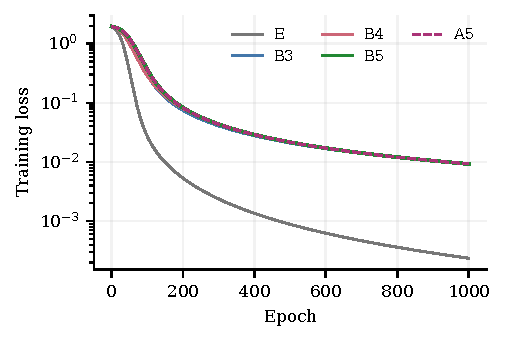
\includegraphics[width=.49\linewidth]{figures/fig_loss_revision_cora.pdf}
\caption{Complete 1000-epoch Cora/GCN training-loss trajectories, with a logarithmic loss axis. Scores are tabulated in Table~\ref{tab:revision-cora}; test data do not select these curves or their run length.}
\label{fig:loss-cora}
\end{figure}

B5 final test accuracy is 0.772 versus 0.771 for B3, and A5 equals B5 at the reported precision. The Euclidean head reaches 0.778. This is a near-tie among the manifold variants, not evidence of a robust graph-family win or an independent transport benefit. Recorded training times are descriptive and include concurrently running jobs; they are not controlled speed benchmarks. The full trajectories and checkpoints remain available for validation-selected analysis.

The new implementation uses actual Lorentz point parameters with closed-form exponential updates and parallel transport. Curvature gradients differentiate through the point homothety, unlike a partial derivative at fixed ambient coordinates. Classification uses one manifold prototype per class; text uses deterministic hashed tokens with an MLP or a two-layer Transformer; graph models use GCN, GAT, or GraphSAGE; recommendation uses a four-factor product distance with MF or origin-chart LightGCN propagation; KG uses grouped product states with a distance or transported-translation score. Synthetic product factors partition the requested total intrinsic dimension. This last architecture differs from the historical independent-tree groups, and the two protocols are not pooled.

KG evaluation in the revision ranks both heads and tails against every entity, filters other known true triples, uses average ranks for ties, and evaluates fixed full splits. MovieLens and Amazon Books use chronological leave-last-two-out per user. Recommendation excludes observed training items from negative draws and evaluates all-item, user-macro Recall@20/NDCG@20 with observed items masked. Yelp2018 instead preserves its published multi-positive test split, with one seed-42 original training interaction per user held out for validation. All test positives for each user contribute to Recall and normalized DCG. Both Euclidean and Lorentz LightGCN variants use two propagation layers; their geometry differs, while the graph operator is retained in both. Reuters retains all labels and uses binary cross entropy with micro/macro F1. Continual-learning experiments train for 1000 total epochs across five ordered tasks and report task-boundary average accuracy and forgetting; Rotated MNIST uses angles $0,36,72,108,144$ degrees, while Split CIFAR-100 uses five disjoint blocks of 20 class labels. No replay buffer is added. These protocols are predeclared in the executable configuration rather than adjusted after test scores are observed.

Appendix~\ref{app:run-ledger} contains the generated completion ledger and current coverage counts; all 705 retained configurations are complete, while 188 deferred configurations are excluded from completion claims. Original WN18RR, FB15k-237, and MNIST data were recovered from the hpc project directory. Tiny-ImageNet and YAGO3-10 have been acquired separately. The deterministic Amazon Books 20K-user subset has also been acquired from the official 2018 five-core release. An existing compute environment ImageNet-100 cache has now been located and its manifest verified: 114129 training images, 12560 held-out training images for validation, and 5000 official validation images reserved as test. This is the cached \texttt{clane9/imagenet-100} version with shorter-side-160px source images, subsequently resized by the declared input transform; it must not be conflated with an original-resolution protocol. The manifest hash and data source are retained with the execution records. Its 18 formerly blocked configurations were made runnable before the budget amendment and are now explicitly deferred. The Yelp subset is instantiated as the Yelp2018 interaction benchmark released by the LightGCN authors \citep{he2020lightgcn}, rather than an unspecified raw-review subset. It contains 31668 users, 38048 items, 1205591 retained training interactions, 31668 validation interactions, and 324147 original test interactions. The source commit and file hashes are recorded; the original test split is unchanged. This explicitly named, non-chronological protocol resolved the twelve data-blocked configurations; their execution is now deferred under the same budget amendment.


\subsection{Complete paired graph comparisons}
Table~\ref{tab:revision-breadth} extends the graph comparison beyond Cora. The generated table contains every dataset--encoder pair for which both B3 and B5 have completed the same 1000-epoch protocol. It uses final test accuracy consistently; validation-selected test metrics are retained separately in the machine-readable evidence file. Positive, tied, and negative differences are all kept. A positive single-seed difference is descriptive evidence for that configuration, not a significance claim or a substitute for equal-budget hyperparameter tuning.

% WWW_REFERENCE_STYLE
\begin{table*}[t]
\centering
\footnotesize\setlength{\tabcolsep}{4.2pt}\renewcommand{\arraystretch}{1.12}
\caption{Completed graph comparisons on compute environment, seed 42, 1000 epochs. Final test accuracy (\%) is the common endpoint; $\Delta$ is B5 minus B3 in percentage points. Every dataset--encoder pair with both completed runs is shown, including ties and negative differences. E is an architecture control with a Euclidean linear head. Dashes mean a comparator has not finished.}
\label{tab:revision-breadth}
\begin{adjustbox}{max width=\linewidth}
\begin{tabular}{llrrrrr}
\toprule
Dataset & Encoder & E & B3 & B5 & A5 & $\Delta$ \\
\midrule
arxiv & gat & \textbf{68.42} & 62.33 & \cellcolor{oursbg}62.41 & 62.45 & +0.08 \\
arxiv & gcn & \textbf{67.66} & 61.34 & \cellcolor{oursbg}61.19 & 61.21 & -0.16 \\
arxiv & sage & \textbf{68.32} & 63.39 & \cellcolor{oursbg}63.67 & 63.50 & +0.28 \\
citeseer & gat & \textbf{65.80} & 64.70 & \cellcolor{oursbg}64.60 & 64.60 & -0.10 \\
citeseer & gcn & 63.70 & \textbf{65.60} & \cellcolor{oursbg}\textbf{65.60} & \textbf{65.60} & +0.00 \\
citeseer & sage & 62.30 & 66.50 & \cellcolor{oursbg}\textbf{66.60} & \textbf{66.60} & +0.10 \\
cora & gat & 66.60 & \textbf{67.90} & \cellcolor{oursbg}67.70 & 67.70 & -0.20 \\
cora & gcn & \textbf{77.80} & 77.10 & \cellcolor{oursbg}77.20 & 77.20 & +0.10 \\
cora & sage & 77.80 & \textbf{78.10} & \cellcolor{oursbg}78.00 & 78.00 & -0.10 \\
pubmed & gat & 71.80 & \textbf{75.90} & \cellcolor{oursbg}\textbf{75.90} & \textbf{75.90} & +0.00 \\
pubmed & gcn & \textbf{76.50} & 75.90 & \cellcolor{oursbg}75.90 & 75.90 & +0.00 \\
pubmed & sage & 74.20 & 75.10 & \cellcolor{oursbg}\textbf{75.20} & \textbf{75.20} & +0.10 \\
\bottomrule
\end{tabular}
\end{adjustbox}
\end{table*}


\subsection{Long-horizon classification, ranking, and retention audit}
\label{app:long-horizon-audit}
We distinguish a complete method block from individual full-length runs. The 20 Newsgroups pooled-token block contains all eight registered methods. Its separate Transformer block has six registered methods; WN18RR translation, MovieLens-1M, and Rotated MNIST each have eight. WN18RR distance has six registered methods. These tables include only completed runs and state their coverage; missing controls are not assigned scores. Deferred methods are counted separately from unfinished retained controls. All records use seed 42 and the registered stopping length. Raw result and trajectory digests, selected validation epochs, and available per-run source digests are retained in \texttt{tables/revision\_long\_horizon\_evidence.json}. These are descriptive comparisons of registered configurations, not a claim that every run has an identical complete source snapshot.

\paragraph{Text classification and checkpoint selection.}
The registry name \texttt{mlp} denotes a pooled-token encoder: deterministic lowercase word hashing into 29999 nonpadding token IDs, truncation to 256 tokens, learned 128-dimensional token embeddings, masked mean pooling, and a 32-dimensional linear projection. The official 20 Newsgroups training split is divided into 10182 training and 1132 stratified validation documents with seed 42; all 7532 official test documents are retained. Headers, footers, and quotes are removed. The encoder uses AdamW with step $10^{-3}$; geometric prototypes use base step $0.1$, curvature step $0.001$, momentum $0.9$, and initial curvature 1. These are fixed configurations, not a hyperparameter search. Validation accuracy is checked every epoch; the first maximizing checkpoint is selected after the complete 1000-epoch run, and its test scores are distinguished from the final checkpoint. All eight selected epochs have been checked against the raw validation trajectories.

% WWW_REFERENCE_STYLE
\begin{table}[!htbp]
\centering
\caption{\textbf{Complete 20 Newsgroups classification block.} Eight methods, 1000 epochs each, seed 42. The registry labels the pooled-token encoder as \texttt{mlp}. The first maximum validation-accuracy checkpoint selects each method\textquotesingle s test result; epochs are one-based. All scores are percentages. Final accuracy is a separately labeled endpoint, not an alternative selection rule.}
\label{tab:revision-text-audit}
\footnotesize\setlength{\tabcolsep}{5pt}\renewcommand{\arraystretch}{1.12}
\begin{tabular}{lrrrrr}
\toprule
Method & Selected epoch & Val. acc.\ $\uparrow$ & Test acc.\ $\uparrow$ & Test macro-F1\ $\uparrow$ & Final acc.\ $\uparrow$ \\
\midrule
E & 427 & \textbf{71.113} & \textbf{61.471} & \textbf{60.750} & \textbf{61.418} \\
B2 & 179 & 68.463 & 57.554 & 56.291 & 56.678 \\
B3 & 179 & 68.728 & 57.820 & 56.552 & 56.745 \\
B4 & 183 & 68.286 & 57.754 & 56.494 & 56.121 \\
\rowcolor{oursbg}
B5 & 182 & 68.551 & 57.674 & 56.449 & 56.213 \\
A5 & 182 & 68.551 & 57.687 & 56.461 & 56.213 \\
B35 & 179 & 68.728 & 57.820 & 56.560 & 56.798 \\
Shared & 179 & 68.728 & 57.674 & 56.457 & 56.028 \\
\bottomrule
\end{tabular}
\end{table}


\paragraph{Separate Transformer comparison.}
The Transformer retains the same tokenization, data partitions, output dimension, prototype configuration, and validation selection. It adds learned positional embeddings and two Transformer encoder layers, each with hidden dimension 128, four attention heads, feed-forward dimension 256, and zero dropout, before masked mean pooling and projection. Table~\ref{tab:revision-transformer-audit} reports all four retained methods, including the B3--B5 pair. The two runs record identical hashes for the runner, geometry, and structured-task source modules. Their validation maxima occur at epochs 648 and 451, respectively (one-based). Selected test accuracy is $54.673\%$ for B3 and $52.987\%$ for B5, a B5 difference of $-1.686$ percentage points; selected macro-F1 is also lower for B5. Final accuracy preserves this ordering. The E and A5 controls finish at validation-selected test accuracies $55.709\%$ and $54.169\%$, respectively. Thus all four retained methods are complete, while B2 and B4 remain deferred. A different encoder on the same dataset is not an independent task family.

% WWW_REFERENCE_STYLE
\begin{table}[!htbp]
\centering
\caption{\textbf{20 Newsgroups Transformer: completed method endpoints.} Each listed method finishes 1000 epochs, seed 42. The first maximum validation-accuracy checkpoint selects its test result; epochs are one-based. 4/6 registered methods complete; 2 methods deferred by the budget amendment. Every completed method is retained. All scores are percentages; final accuracy is separately labeled. Bold compares only the displayed rows; B5 is shaded.}
\label{tab:revision-transformer-audit}
\footnotesize\setlength{\tabcolsep}{5pt}\renewcommand{\arraystretch}{1.12}
\begin{tabular}{lrrrrr}
\toprule
Method & Selected epoch & Val. acc.\ $\uparrow$ & Test acc.\ $\uparrow$ & Test macro-F1\ $\uparrow$ & Final acc.\ $\uparrow$ \\
\midrule
E & 960 & \textbf{65.724} & \textbf{55.709} & \textbf{55.006} & \textbf{55.616} \\
B3 & 648 & 63.428 & 54.673 & 53.539 & 54.408 \\
\rowcolor{oursbg}
B5 & 451 & 61.749 & 52.987 & 52.485 & 52.894 \\
A5 & 592 & 62.544 & 54.169 & 53.213 & 53.120 \\
\bottomrule
\end{tabular}
\end{table}


\paragraph{Primary endpoints in the other registered families.}
Tables~\ref{tab:revision-kg-audit}--\ref{tab:revision-retention-audit} report final endpoints rather than substituting the best observed test checkpoint. WN18RR translation B5 MRR is $0.10230$, versus $0.17225$ for E, $0.12598$ for B3, $0.12596$ for B35, and $0.10232$ for B4; B5 and A5 agree at the displayed precision. On MovieLens-1M, B5 Recall@20 is slightly higher than B3, but the primary NDCG@20 is lower ($2.1560\%$ versus $2.2072\%$); E reaches $4.2943\%$. On Rotated MNIST, all eight methods are complete. B5 mean accuracy is $43.432\%$, versus $43.388\%$ for B35 and $43.296\%$ for shared curvature: small increases of $0.044$ and $0.136$ percentage points. However, E, B3, and B2 reach $43.800\%$, $43.752\%$, and $44.340\%$, respectively. Shared curvature gives the highest last-task accuracy, $98.530\%$, versus $98.470\%$ for B5. A last-task score does not measure retention of earlier tasks. Accordingly, these observations do not establish an additional positive task family or an isolated transport benefit. All completed primary and secondary endpoints are shown, with each deferred method explicitly identified.

The completed shared-curvature WN18RR control has MRR $0.10200$. Grouped B5 improves this narrowly by $0.000295$ absolute MRR ($0.289\%$ relative), while remaining below both fixed-curvature controls; Hits@10 is slightly lower than shared curvature ($30.600\%$ versus $30.616\%$). This mixed profile does not establish a broad grouped-curvature gain. The MovieLens-1M A5 endpoint equals B5 exactly in both stored primary NDCG@20 ($0.02156021$) and secondary Recall@20 ($0.05546358$). Equality is an observed ranking-score result for this run, not a claim that the optimizer trajectories are identical. Primary endpoint choice, full run lengths, and the original configurations are unchanged.

% WWW_REFERENCE_STYLE
\begin{table}[!htbp]
\centering
\caption{\textbf{Available full-length endpoints.} WN18RR transported-translation model, 2000 epochs. All-entity filtered head-and-tail ranking at the final checkpoint. MRR is primary; Hits scores are percentages. 7/8 registered methods complete; all completed rows are shown. 1 method is deferred by the budget amendment. Bold compares only the displayed completed rows, including rounded ties; B5 is shaded. Seed 42, fixed starting configuration, no equal-budget hyperparameter search.}
\label{tab:revision-kg-audit}
\footnotesize\setlength{\tabcolsep}{5pt}\renewcommand{\arraystretch}{1.12}
\begin{tabular}{lrrrr}
\toprule
Method & MRR $\uparrow$ & Hits@1 (\%) $\uparrow$ & Hits@3 (\%) $\uparrow$ & Hits@10 (\%) $\uparrow$ \\
\midrule
E & \textbf{0.17225} & 0.271 & \textbf{30.568} & \textbf{45.246} \\
B3 & 0.12598 & \textbf{2.106} & 18.427 & 35.354 \\
B4 & 0.10232 & 1.133 & 15.077 & 30.632 \\
\rowcolor{oursbg}
B5 & 0.10230 & 1.133 & 15.061 & 30.600 \\
A5 & 0.10230 & 1.133 & 15.061 & 30.600 \\
B35 & 0.12596 & \textbf{2.106} & 18.427 & 35.354 \\
Shared & 0.10200 & 1.101 & 14.853 & 30.616 \\
\bottomrule
\end{tabular}
\end{table}

% WWW_REFERENCE_STYLE
\begin{table}[!htbp]
\centering
\caption{\textbf{Available full-length endpoints.} MovieLens-1M product-distance MF, 1000 epochs. Final all-item user-macro scores after chronological splitting and observed-item masking. NDCG@20 is primary; Recall@20 is secondary. Both are percentages. 5/8 registered methods complete; all completed rows are shown. 3 methods are deferred by the budget amendment. Bold compares only the displayed completed rows, including rounded ties; B5 is shaded. Seed 42, fixed starting configuration, no equal-budget hyperparameter search.}
\label{tab:revision-recommendation-audit}
\footnotesize\setlength{\tabcolsep}{5pt}\renewcommand{\arraystretch}{1.12}
\begin{tabular}{lrr}
\toprule
Method & NDCG@20 $\uparrow$ & Recall@20 $\uparrow$ \\
\midrule
E & \textbf{4.2943} & \textbf{11.5563} \\
B3 & 2.2072 & 5.4967 \\
\rowcolor{oursbg}
B5 & 2.1560 & 5.5464 \\
A5 & 2.1560 & 5.5464 \\
B35 & 2.2069 & 5.4967 \\
\bottomrule
\end{tabular}
\end{table}

% WWW_REFERENCE_STYLE
\begin{table}[!htbp]
\centering
\caption{\textbf{Available full-length endpoints.} Rotated MNIST, five ordered tasks and 1000 total epochs without replay. Mean accuracy across all five tasks is primary; forgetting averages the first four tasks, in percentage points. Last-task accuracy is secondary. All rows use the final checkpoint. 8/8 registered methods complete; all completed rows are shown. Bold compares only the displayed completed rows, including rounded ties; B5 is shaded. Seed 42, fixed starting configuration, no equal-budget hyperparameter search.}
\label{tab:revision-retention-audit}
\footnotesize\setlength{\tabcolsep}{5pt}\renewcommand{\arraystretch}{1.12}
\begin{tabular}{lrrr}
\toprule
Method & Mean acc. (\%) $\uparrow$ & Forgetting (pp) $\downarrow$ & Last-task acc. (\%) $\uparrow$ \\
\midrule
E & 43.800 & 68.267 & 98.380 \\
B2 & \textbf{44.340} & \textbf{67.520} & 98.350 \\
B3 & 43.752 & 68.320 & 98.390 \\
B4 & 42.804 & 69.535 & 98.390 \\
\rowcolor{oursbg}
B5 & 43.432 & 68.715 & 98.470 \\
A5 & 43.378 & 68.782 & 98.350 \\
B35 & 43.388 & 68.807 & 98.400 \\
Shared & 43.296 & 68.927 & \textbf{98.530} \\
\bottomrule
\end{tabular}
\end{table}

\FloatBarrier

\subsection{Budget amendment and retained comparisons}
\label{app:scope-amendment}
On November 4, 2026, the remaining execution budget was reduced after 691 of the 893 registered configurations had completed. The decision used the observed outcomes and compute costs and is therefore exploratory. Of the 202 unfinished configurations, 14 are retained and 188 deferred. Table~\ref{tab:scope-amendment} enumerates every retained unfinished comparison. It preserves ongoing controls, supplies three missing Euclidean anchors, and completes one unopened model block with all six original methods. No completed result is excluded; the registry, raw trajectories, and intermediate checkpoints remain available. The amendment is recorded in \texttt{experiments/revision/execution\_scope.json} and linked to each deferred record.

\begin{table}[!htbp]
\centering
\caption{Remaining execution budget at the amendment. Counts refer to unfinished configurations on November 4, not new trials or completed results. All retained runs keep their registered seed, splits, settings, and full training length.}
\label{tab:scope-amendment}
\footnotesize\setlength{\tabcolsep}{5pt}\renewcommand{\arraystretch}{1.12}
\begin{tabular}{llrr}
\toprule
Dataset and model & Retained unfinished methods & Runs & Epochs \\
\midrule
Rotated MNIST / MLP & B35, shared & 2 & 1000 \\
20 Newsgroups / Transformer & A5, E & 2 & 1000 \\
MovieLens-1M / MF & B35, E & 2 & 1000 \\
WN18RR / translation & B4, E & 2 & 2000 \\
WN18RR / distance & E, B2, B3, B4, B5, A5 & 6 & 2000 \\
\midrule
Total retained unfinished & & 14 & \\
Deferred, never started & & 187 & \\
Deferred, partially trained & CIFAR-100 / ResNet-18 / B5 & 1 & \\
\bottomrule
\end{tabular}
\end{table}

The interrupted CIFAR-100 run is not reported as a completed visual benchmark or a numerical failure. Its available checkpoints and loss log are preserved. The broad dataset--encoder expansion and other unstarted ablations are deferred for budget reasons. Within the amended blocks, the retained method counts are four of six for the Transformer, seven of eight for WN18RR translation, five of eight for MovieLens-1M, and all eight for Rotated MNIST. All 705 retained configurations have now completed, including all 14 runs retained by this amendment. The original 893 registrations are not relabeled as completed; the 188 deferred configurations remain separately identified.

\paragraph{Hierarchy-motivated distance comparison.}
The retained WN18RR distance block replaces transported translation by a relation-weighted product-distance score,
\begin{equation*}
s(h,r,t)=-\sum_{g=1}^{4}\bigl(1+\|v_{r,g}\|_{K_g}^{2}\bigr)
d_{K_g}(x_{h,g},x_{t,g})^2,
\qquad v_{r,g}=\operatorname{Log}_{o_{K_g}}(x_{r,g}).
\end{equation*}
It directly tests metric fitting on the same hierarchical graph, with the matched Euclidean architecture replacing each factor distance and relation norm by their Euclidean counterparts. All six originally registered methods are retained together, including the Euclidean, fixed-curvature, and no-transport controls; no hyperparameter or stopping rule is changed to pursue a favorable endpoint. The score is symmetric in its entity arguments, so it does not itself encode edge direction. This is a model-specific test within KG completion, not an additional task family. MRR remains the primary final-checkpoint endpoint under full filtered head-and-tail ranking, and the existing single-seed qualification remains in force. All six methods have now completed 2000 epochs. Table~\ref{tab:revision-kg-distance-audit} gives B5 MRR $0.13685$, compared with $0.15722$ for E, $0.14078$ for B2, $0.14077$ for B3, $0.13688$ for B4, and $0.13691$ for A5. B5 does not improve the primary endpoint over any of these controls. Its higher Hits@3 than B2 and B3 does not reverse the MRR or Hits@10 comparison. These final results do not establish an additional task-family advantage.

% WWW_REFERENCE_STYLE
\begin{table}[!htbp]
\centering
\caption{\textbf{Available full-length endpoints.} WN18RR relation-weighted distance model, 2000 epochs. All six registered methods are retained under the budget amendment. All-entity filtered head-and-tail ranking at the final checkpoint. MRR is primary; Hits scores are percentages. 6/6 registered methods complete; all completed rows are shown. Bold compares only the displayed completed rows, including rounded ties; B5 is shaded. Seed 42, fixed starting configuration, no equal-budget hyperparameter search.}
\label{tab:revision-kg-distance-audit}
\footnotesize\setlength{\tabcolsep}{5pt}\renewcommand{\arraystretch}{1.12}
\begin{tabular}{lrrrr}
\toprule
Method & MRR $\uparrow$ & Hits@1 (\%) $\uparrow$ & Hits@3 (\%) $\uparrow$ & Hits@10 (\%) $\uparrow$ \\
\midrule
E & \textbf{0.15722} & \textbf{0.000} & \textbf{30.089} & \textbf{38.449} \\
B2 & 0.14078 & \textbf{0.000} & 25.973 & 37.572 \\
B3 & 0.14077 & \textbf{0.000} & 25.973 & 37.556 \\
B4 & 0.13688 & \textbf{0.000} & 27.361 & 34.923 \\
\rowcolor{oursbg}
B5 & 0.13685 & \textbf{0.000} & 27.393 & 34.907 \\
A5 & 0.13691 & \textbf{0.000} & 27.393 & 34.907 \\
\bottomrule
\end{tabular}
\end{table}

\FloatBarrier


\subsection{Complete product-factor reconstruction grid}
\label{app:complete-product-grid}
The four tree constructions are binary, 4-ary, 8-ary, and variable-branching trees. Each uses the full Cartesian grid of three node counts and four total intrinsic dimensions stated in Table~\ref{tab:revision-synthetic-complete}. The Lorentz product has $\min(4,d)$ factors whose dimensions sum to $d$; every factor fits the same tree observations. Each update samples 65536 ordered node pairs, removes self-pairs, and minimizes mean squared relative-distance error. A separate generator fixed at seed 1042 draws up to 100000 evaluation pairs once, again removing self-pairs; final distortion is mean absolute relative-distance error on that fixed set. This is a reconstruction diagnostic: evaluation pairs are not withheld from the training-pair distribution. All methods finish 2000 updates. The Euclidean control uses SGD with momentum 0.9 and step 10; the manifold methods use base step 10, curvature step 0.001, and the common geometric safeguards. This is a fixed-configuration comparison, not a validation-selected tuning study. In particular, the B5--B3 contrast combines curvature adaptation and step normalization, while B5--A5 isolates the cross-curvature state map. The full table makes both contrasts and the Euclidean result inspectable.
% WWW_REFERENCE_STYLE
\begingroup
\footnotesize\setlength{\tabcolsep}{4.2pt}\renewcommand{\arraystretch}{1.12}
\begin{longtable}{lrrrrrrrrr}
\caption{Complete product-factor reconstruction grid. Final fixed-pair distortion (lower is better) after 2000 updates, seed 42. Bold indicates the best value at the displayed precision; B5 is shaded. The last column reports the B5 reduction relative to B3 in percent, calculated from unrounded records. All baselines, including the stronger Euclidean control, are retained.}\label{tab:revision-synthetic-all}\\
\toprule
Tree & $n$ & $d$ & E & B2 & B3 & B4 & B5 & A5 & Reduction (\%) \\
\midrule
\endfirsthead
\toprule
Tree & $n$ & $d$ & E & B2 & B3 & B4 & B5 & A5 & Reduction (\%) \\
\midrule
\endhead
\bottomrule
\endfoot
Binary & 1000 & 2 & \textbf{0.41637} & 0.72640 & 0.72635 & 0.72403 & \cellcolor{oursbg}0.72399 & 0.72400 & 0.3247 \\
Binary & 1000 & 5 & \textbf{0.32602} & 0.66094 & 0.66133 & 0.65903 & \cellcolor{oursbg}0.65943 & 0.65945 & 0.2874 \\
Binary & 1000 & 10 & \textbf{0.29453} & 0.63097 & 0.63134 & 0.62930 & \cellcolor{oursbg}0.62969 & 0.62970 & 0.2620 \\
Binary & 1000 & 20 & \textbf{0.27958} & 0.61316 & 0.61350 & 0.61161 & \cellcolor{oursbg}0.61197 & 0.61198 & 0.2505 \\
Binary & 5000 & 2 & \textbf{0.69453} & 0.95452 & 0.95471 & 0.95440 & \cellcolor{oursbg}0.95459 & 0.95459 & 0.0125 \\
Binary & 5000 & 5 & \textbf{0.65076} & 0.94672 & 0.94693 & 0.94662 & \cellcolor{oursbg}0.94683 & 0.94683 & 0.0099 \\
Binary & 5000 & 10 & \textbf{0.63689} & 0.94239 & 0.94261 & 0.94229 & \cellcolor{oursbg}0.94250 & 0.94250 & 0.0111 \\
Binary & 5000 & 20 & \textbf{0.62965} & 0.93826 & 0.93848 & 0.93814 & \cellcolor{oursbg}0.93836 & 0.93836 & 0.0127 \\
Binary & 10000 & 2 & \textbf{0.84620} & 0.98018 & 0.98026 & 0.98016 & \cellcolor{oursbg}0.98024 & 0.98024 & 0.0026 \\
Binary & 10000 & 5 & \textbf{0.82480} & 0.97607 & 0.97616 & 0.97605 & \cellcolor{oursbg}0.97614 & 0.97614 & 0.0022 \\
Binary & 10000 & 10 & \textbf{0.81708} & 0.97329 & 0.97338 & 0.97327 & \cellcolor{oursbg}0.97336 & 0.97336 & 0.0028 \\
Binary & 10000 & 20 & \textbf{0.81226} & 0.97009 & 0.97018 & 0.97005 & \cellcolor{oursbg}0.97014 & 0.97014 & 0.0036 \\
4-ary & 1000 & 2 & \textbf{0.36051} & 0.50908 & 0.50823 & 0.50512 & \cellcolor{oursbg}0.50421 & 0.50422 & 0.7910 \\
4-ary & 1000 & 5 & \textbf{0.23455} & 0.38139 & 0.38131 & 0.37882 & \cellcolor{oursbg}0.37876 & 0.37878 & 0.6707 \\
4-ary & 1000 & 10 & \textbf{0.18215} & 0.34137 & 0.34100 & 0.33942 & \cellcolor{oursbg}0.33906 & 0.33907 & 0.5688 \\
4-ary & 1000 & 20 & \textbf{0.15829} & 0.32290 & 0.32242 & 0.32127 & \cellcolor{oursbg}0.32080 & 0.32081 & 0.5012 \\
4-ary & 5000 & 2 & \textbf{0.44106} & 0.87753 & 0.87796 & 0.87673 & \cellcolor{oursbg}0.87717 & 0.87717 & 0.0901 \\
4-ary & 5000 & 5 & \textbf{0.34468} & 0.85667 & 0.85718 & 0.85606 & \cellcolor{oursbg}0.85657 & 0.85657 & 0.0713 \\
4-ary & 5000 & 10 & \textbf{0.31659} & 0.84622 & 0.84675 & 0.84557 & \cellcolor{oursbg}0.84611 & 0.84611 & 0.0761 \\
4-ary & 5000 & 20 & \textbf{0.30328} & 0.83768 & 0.83823 & 0.83698 & \cellcolor{oursbg}0.83754 & 0.83754 & 0.0828 \\
4-ary & 10000 & 2 & \textbf{0.62564} & 0.94424 & 0.94446 & 0.94405 & \cellcolor{oursbg}0.94427 & 0.94427 & 0.0195 \\
4-ary & 10000 & 5 & \textbf{0.57078} & 0.93405 & 0.93430 & 0.93390 & \cellcolor{oursbg}0.93415 & 0.93415 & 0.0159 \\
4-ary & 10000 & 10 & \textbf{0.55361} & 0.92822 & 0.92847 & 0.92805 & \cellcolor{oursbg}0.92830 & 0.92831 & 0.0183 \\
4-ary & 10000 & 20 & \textbf{0.54395} & 0.92227 & 0.92253 & 0.92207 & \cellcolor{oursbg}0.92233 & 0.92233 & 0.0218 \\
8-ary & 1000 & 2 & \textbf{0.34629} & 0.39497 & 0.39423 & 0.39353 & \cellcolor{oursbg}0.39280 & 0.39281 & 0.3624 \\
8-ary & 1000 & 5 & \textbf{0.18629} & 0.24986 & 0.24962 & 0.24934 & \cellcolor{oursbg}0.24911 & 0.24912 & 0.2061 \\
8-ary & 1000 & 10 & \textbf{0.12706} & 0.21326 & 0.21275 & 0.21273 & \cellcolor{oursbg}0.21224 & 0.21225 & 0.2371 \\
8-ary & 1000 & 20 & \textbf{0.09254} & 0.19817 & 0.19757 & 0.19764 & \cellcolor{oursbg}0.19706 & 0.19706 & 0.2576 \\
8-ary & 5000 & 2 & \textbf{0.36754} & 0.78506 & 0.78563 & 0.78287 & \cellcolor{oursbg}0.78345 & 0.78346 & 0.2768 \\
8-ary & 5000 & 5 & \textbf{0.23428} & 0.74700 & 0.74772 & 0.74530 & \cellcolor{oursbg}0.74603 & 0.74605 & 0.2255 \\
8-ary & 5000 & 10 & \textbf{0.19336} & 0.72832 & 0.72909 & 0.72659 & \cellcolor{oursbg}0.72737 & 0.72738 & 0.2360 \\
8-ary & 5000 & 20 & \textbf{0.17304} & 0.71503 & 0.71583 & 0.71324 & \cellcolor{oursbg}0.71405 & 0.71406 & 0.2498 \\
8-ary & 10000 & 2 & \textbf{0.46059} & 0.89895 & 0.89931 & 0.89837 & \cellcolor{oursbg}0.89874 & 0.89874 & 0.0634 \\
8-ary & 10000 & 5 & \textbf{0.37142} & 0.88138 & 0.88180 & 0.88093 & \cellcolor{oursbg}0.88135 & 0.88135 & 0.0509 \\
8-ary & 10000 & 10 & \textbf{0.34542} & 0.87208 & 0.87252 & 0.87159 & \cellcolor{oursbg}0.87203 & 0.87203 & 0.0565 \\
8-ary & 10000 & 20 & \textbf{0.33156} & 0.86344 & 0.86388 & 0.86288 & \cellcolor{oursbg}0.86333 & 0.86333 & 0.0646 \\
Variable & 1000 & 2 & \textbf{0.37559} & 0.56828 & 0.56758 & 0.56467 & \cellcolor{oursbg}0.56395 & 0.56396 & 0.6402 \\
Variable & 1000 & 5 & \textbf{0.24945} & 0.45533 & 0.45542 & 0.45274 & \cellcolor{oursbg}0.45283 & 0.45285 & 0.5673 \\
Variable & 1000 & 10 & \textbf{0.21387} & 0.41568 & 0.41553 & 0.41362 & \cellcolor{oursbg}0.41348 & 0.41350 & 0.4926 \\
Variable & 1000 & 20 & \textbf{0.19139} & 0.39677 & 0.39651 & 0.39501 & \cellcolor{oursbg}0.39476 & 0.39477 & 0.4425 \\
Variable & 5000 & 2 & \textbf{0.51448} & 0.90613 & 0.90648 & 0.90565 & \cellcolor{oursbg}0.90600 & 0.90600 & 0.0529 \\
Variable & 5000 & 5 & \textbf{0.43579} & 0.89022 & 0.89062 & 0.88984 & \cellcolor{oursbg}0.89025 & 0.89025 & 0.0416 \\
Variable & 5000 & 10 & \textbf{0.41323} & 0.88205 & 0.88248 & 0.88165 & \cellcolor{oursbg}0.88208 & 0.88208 & 0.0449 \\
Variable & 5000 & 20 & \textbf{0.40134} & 0.87510 & 0.87553 & 0.87466 & \cellcolor{oursbg}0.87510 & 0.87510 & 0.0496 \\
Variable & 10000 & 2 & \textbf{0.68836} & 0.95593 & 0.95611 & 0.95582 & \cellcolor{oursbg}0.95599 & 0.95599 & 0.0123 \\
Variable & 10000 & 5 & \textbf{0.64379} & 0.94772 & 0.94792 & 0.94763 & \cellcolor{oursbg}0.94782 & 0.94782 & 0.0101 \\
Variable & 10000 & 10 & \textbf{0.62919} & 0.94285 & 0.94305 & 0.94273 & \cellcolor{oursbg}0.94294 & 0.94294 & 0.0118 \\
Variable & 10000 & 20 & \textbf{0.62107} & 0.93769 & 0.93790 & 0.93755 & \cellcolor{oursbg}0.93776 & 0.93776 & 0.0144 \\
\end{longtable}
\endgroup


\subsection{All long-horizon mechanism conditions}
% WWW_REFERENCE_STYLE
\begin{table*}[t]
\centering
\footnotesize\setlength{\tabcolsep}{4.2pt}\renewcommand{\arraystretch}{1.12}
\caption{Long-horizon hierarchy mechanism tests: final held-out pair distortion after 2000 updates (lower is better). All methods use seed 42 and identical pair splits. Only cases with completed B5, B3, and A5 are included. The best-fixed column requires all five B35 curvature settings and selects using final validation distortion, never test distortion. Missing comparisons remain dashes. These controlled synthetic cases are not additional real-data task families.}
\label{tab:revision-mechanism}
\begin{adjustbox}{max width=\linewidth}
\begin{tabular}{lrrrrrr}
\toprule
Case & B3 & B5 & A5 & Shared & B4 & Best fixed \\
\midrule
abrupt8 & 0.7417 & \cellcolor{oursbg}0.6176 & 0.6176 & 0.6143 & 0.5914 & \textbf{0.1637} \\
heterogeneous & 0.2510 & \cellcolor{oursbg}0.2470 & 0.2463 & 0.2543 & 0.2415 & \textbf{0.2182} \\
smooth2 & 0.3328 & \cellcolor{oursbg}0.3295 & 0.3296 & 0.3260 & 0.3202 & \textbf{0.1823} \\
smooth5 & 0.6225 & \cellcolor{oursbg}0.4347 & 0.4347 & 0.4479 & 0.4262 & \textbf{0.2058} \\
smooth8 & 0.7411 & \cellcolor{oursbg}0.4813 & 0.4813 & 0.5078 & 0.4719 & \textbf{0.2757} \\
static & 0.2734 & \cellcolor{oursbg}0.2727 & 0.2726 & 0.2785 & 0.2604 & \textbf{0.2011} \\
\bottomrule
\end{tabular}
\end{adjustbox}
\end{table*}

% WWW_REFERENCE_STYLE
\begin{table*}[t]
\centering
\footnotesize\setlength{\tabcolsep}{4.2pt}\renewcommand{\arraystretch}{1.12}
\caption{Matched five-initialization comparison, 2000 updates per run. B35, B5, and A5 each use $K_0\in\{0.03,0.1,0.3,1,3\}$, with configurations selected by final validation distortion. Test distortion is reported after selection. A case appears only when all 15 runs finish. The last column compares B5 with A5 at B5\textquotesingle s selected initialization, retaining the clean transport contrast.}
\label{tab:revision-selected-mechanism}
\begin{adjustbox}{max width=\linewidth}
\begin{tabular}{lrrrrr}
\toprule
Case & Best fixed & B5 & Best A5 & B5 $K_0$ & Matched A5 \\
\midrule
abrupt8 & \textbf{0.1637} & \cellcolor{oursbg}0.1655 & 0.1663 & 0.03 & 0.1663 \\
heterogeneous & 0.2182 & \cellcolor{oursbg}0.2177 & \textbf{0.2174} & 0.1 & \textbf{0.2174} \\
smooth2 & 0.1823 & \cellcolor{oursbg}\textbf{0.1762} & 0.1763 & 0.1 & 0.1763 \\
smooth5 & \textbf{0.2058} & \cellcolor{oursbg}\textbf{0.2058} & 0.2061 & 0.03 & 0.2061 \\
smooth8 & 0.2757 & \cellcolor{oursbg}\textbf{0.2619} & 0.2624 & 0.03 & 0.2624 \\
static & 0.2011 & \cellcolor{oursbg}0.1952 & \textbf{0.1951} & 0.1 & \textbf{0.1951} \\
\bottomrule
\end{tabular}
\end{adjustbox}
\end{table*}


\subsection{New real-data protocols and complete comparisons}
The WordNet tasks use the full mammal and vehicle descendant subtrees in WordNet 3.0, including instances, and all internal transitive hypernym relations. The subtrees contain 1182 and 528 synsets, with 6542 and 2311 directed positive pairs, respectively. This is a custom missing-relation protocol and differs from the filtered mammals reconstruction benchmark of \citet{nickel2017poincare}. The corpus is accessed through NLTK \citep{nltkwordnet}. Ten percent of relations are reserved for validation and ten percent for test; the training split retains at least one incident relation for every nonisolated vertex. Filtered macro query MAP ranks every other synset and masks known positives outside the target split. The score penalizes both product distance and a reversed descendant--ancestor radial order.

Cora and Citeseer links use the Planetoid graphs \citep{planetoiddata}, with node identities but no attributes or class labels. Undirected pairs are canonicalized before splitting. Positive and negative pairs are disjoint across train, validation, and test, including reverse-edge equivalence; known positives are excluded from negative draws. The splits contain 5278 and 4552 positive pairs, respectively, with a matched number of negatives and an approximately 80/10/10 positive split that preserves training vertex coverage. Balanced-pair AP is primary and ROC-AUC is secondary; these scores do not estimate precision at the natural all-pairs prevalence.

Optical digits uses the 1797-image dataset distributed by scikit-learn \citep{sklearndigits}, with stratified training/validation/test counts 1078/359/360. Scaling is fit only on training observations. The 20 Newsgroups retrieval task \citep{sklearn20news} retains its official test set and partitions official training documents into 10182 training and 1132 validation queries, with 7532 test queries. Headers, footers, and quotes are removed. TF-IDF with at most 6000 features, a 128-component truncated SVD, and scaling are all fit exclusively on the training partition. A shared 128-unit tanh encoder produces eight features arranged as four two-dimensional factors; class proxies are optimized on their home manifolds. Retrieval uses observation embeddings, not class proxies, and the gallery contains training observations only. Primary same-class Recall@1 is the fraction of queries with a same-label top-ranked gallery item; secondary NDCG@10 uses same-class relevance. These are compact custom retrieval protocols rather than published leaderboard reproductions.

For each manifold method, the six configurations cross $K_0\in\{0.1,1,3\}$ with two base steps: $\{10,100\}$ for relation embeddings and $\{0.1,1\}$ for retrieval proxies. The Euclidean control receives the same two steps crossed with point-decay coefficients $\{0,10^{-4},10^{-2}\}$, also six runs. Other shared settings are $\beta=0.9$, $\rho=0.01$, $K\in[0.001,5]$, the canonical radius cap 4, the normalized trust cap 0.25, and the log-curvature cap 0.01. Auxiliary parameters use AdamW with learning rate $10^{-3}$ and decay $10^{-4}$. Temperature is restricted to $[e^{-3},e^3]$. Full-batch training spans all training examples each epoch. Validation loss is saved every epoch and the primary ranking metric every 25 epochs and at the final checkpoint. Final-checkpoint validation, not the best test score or best test epoch, selects the configuration. Training data, transformations, model capacity, and stopping length are identical across the relevant manifold comparisons. The canonical-radius constraint still makes physical-distance capacity curvature-dependent.

% WWW_REFERENCE_STYLE
Registered new-task completion counts: WordNet mammals: 30/30, Cora links: 30/30, Digits retrieval: 30/30, WordNet vehicles: 30/30, Citeseer links: 30/30, 20News retrieval: 30/30. Test comparison requires the full 30-run block.\par

% WWW_REFERENCE_STYLE
\begin{table*}[t]
\centering
\footnotesize\setlength{\tabcolsep}{4.2pt}\renewcommand{\arraystretch}{1.12}
\caption{Final-checkpoint test scores in percent; higher is better. Taxonomy: filtered query MAP; links: balanced-pair AP; retrieval: same-class Recall@1. Each method selects from six runs by final validation metric; all 30 configurations finish before any test evaluation. Matched A5 uses B5\textquotesingle s selected learning rate and initial curvature. Seed 42; 1000 epochs. Every completed task is retained, including ties and negative differences.}
\label{tab:new-tasks-all}
\begin{adjustbox}{max width=\linewidth}
\begin{tabular}{lrrrrrr}
\toprule
Task & E & B3 & B35 & B5 & A5 & Matched A5 \\
\midrule
WordNet mammals & 8.26 & 8.49 & 8.31 & \cellcolor{oursbg}8.29 & \textbf{8.96} & 8.38 \\
Cora links & \textbf{93.46} & \textbf{93.46} & \textbf{93.46} & \cellcolor{oursbg}\textbf{93.46} & \textbf{93.46} & \textbf{93.46} \\
Digits retrieval & 96.39 & 96.67 & 96.67 & \cellcolor{oursbg}\textbf{96.94} & \textbf{96.94} & \textbf{96.94} \\
WordNet vehicles & 8.42 & 8.40 & 7.80 & \cellcolor{oursbg}\textbf{8.50} & 8.27 & 8.27 \\
Citeseer links & 91.91 & 91.91 & \textbf{91.92} & \cellcolor{oursbg}\textbf{91.92} & \textbf{91.92} & \textbf{91.92} \\
20News retrieval & 42.31 & \textbf{43.49} & \textbf{43.49} & \cellcolor{oursbg}\textbf{43.49} & 43.45 & 43.45 \\
\bottomrule
\end{tabular}
\end{adjustbox}
\end{table*}


\FloatBarrier
\subsection{Recorded non-loss trajectory checkpoints}
\begin{table}[H]
\centering
\caption{\textbf{Historical KG metric checkpoints.} Recorded MRR, Hits@10 and learned curvature spread. Loss alone is plotted in Figure~\ref{fig:kg-loss}.}
\label{tab:kg-checkpoints}
\footnotesize\setlength{\tabcolsep}{4.2pt}\renewcommand{\arraystretch}{1.12}
\begin{adjustbox}{max width=\linewidth}
\begin{tabular}{lrrrrr}
\toprule
Epoch & B3 MRR & B4 MRR & B3 Hits@10 & B4 Hits@10 & B4 $K_{\rm std}$ \\
\midrule
100 & 0.1331 & 0.1334 & 0.3500 & 0.3500 & 0.0765 \\
300 & 0.1386 & 0.1361 & 0.3638 & 0.3688 & 0.2530 \\
500 & 0.1217 & 0.1250 & 0.3463 & 0.3575 & 0.2823 \\
800 & 0.1353 & 0.1384 & 0.3688 & 0.3750 & 0.2867 \\
1000 & 0.1356 & 0.1422 & 0.3588 & 0.3825 & 0.2886 \\
1500 & 0.1323 & 0.1321 & 0.3463 & 0.3538 & 0.2931 \\
1900 & 0.1337 & 0.1326 & 0.3337 & 0.3613 & 0.2946 \\
1999 & 0.1223 & 0.1355 & 0.3500 & 0.3563 & 0.2948 \\
\bottomrule
\end{tabular}
\end{adjustbox}
\end{table}

\begin{table}[H]
\centering
\caption{\textbf{Smooth-drift validation distortion and curvature states.} All methods start at $K_0=1$. $K_1,\ldots,K_4$ are B5 states. These are fixed checkpoints of the complete recorded trajectories, distinct from validation-selected initialization comparisons.}
\label{tab:drift-states}
\footnotesize\setlength{\tabcolsep}{4.2pt}\renewcommand{\arraystretch}{1.12}
\begin{adjustbox}{max width=\linewidth}
\begin{tabular}{lrrrrrrrr}
\toprule
Drift & Update & B3 & B5 & A5 & $K_1$ & $K_2$ & $K_3$ & $K_4$ \\
\midrule
2$\times$ & 1 & \textbf{0.9852} & \cellcolor{oursbg}\textbf{0.9852} & \textbf{0.9852} & 1.000 & 1.000 & 1.000 & 1.000 \\
2$\times$ & 100 & 0.3601 & \cellcolor{oursbg}\textbf{0.3568} & 0.3570 & 1.007 & 1.034 & 1.062 & 1.066 \\
2$\times$ & 500 & 0.3286 & \cellcolor{oursbg}0.3277 & \textbf{0.3276} & 0.978 & 1.052 & 1.082 & 1.096 \\
2$\times$ & 1000 & 0.3230 & \cellcolor{oursbg}0.3217 & \textbf{0.3216} & 0.909 & 1.035 & 1.104 & 1.127 \\
2$\times$ & 2000 & 0.3383 & \cellcolor{oursbg}0.3362 & \textbf{0.3361} & 0.743 & 0.879 & 1.019 & 1.119 \\
5$\times$ & 1 & \textbf{0.9852} & \cellcolor{oursbg}\textbf{0.9852} & \textbf{0.9852} & 1.000 & 1.000 & 1.000 & 1.000 \\
5$\times$ & 100 & 0.3440 & \cellcolor{oursbg}\textbf{0.3425} & \textbf{0.3425} & 1.004 & 1.026 & 1.054 & 1.064 \\
5$\times$ & 500 & \textbf{0.3506} & \cellcolor{oursbg}0.3529 & 0.3529 & 0.951 & 0.983 & 1.035 & 1.063 \\
5$\times$ & 1000 & 0.4660 & \cellcolor{oursbg}\textbf{0.4307} & \textbf{0.4307} & 0.836 & 0.793 & 0.812 & 0.834 \\
5$\times$ & 2000 & 0.6231 & \cellcolor{oursbg}\textbf{0.4382} & \textbf{0.4382} & 0.569 & 0.385 & 0.329 & 0.299 \\
8$\times$ & 1 & \textbf{0.9852} & \cellcolor{oursbg}\textbf{0.9852} & \textbf{0.9852} & 1.000 & 1.000 & 1.000 & 1.000 \\
8$\times$ & 100 & 0.3317 & \cellcolor{oursbg}0.3316 & \textbf{0.3314} & 1.001 & 1.019 & 1.044 & 1.061 \\
8$\times$ & 500 & 0.4446 & \cellcolor{oursbg}\textbf{0.4329} & \textbf{0.4329} & 0.929 & 0.912 & 0.932 & 0.958 \\
8$\times$ & 1000 & 0.5917 & \cellcolor{oursbg}\textbf{0.5123} & \textbf{0.5123} & 0.784 & 0.651 & 0.613 & 0.601 \\
8$\times$ & 2000 & 0.7411 & \cellcolor{oursbg}\textbf{0.4831} & \textbf{0.4831} & 0.444 & 0.223 & 0.165 & 0.138 \\
\bottomrule
\end{tabular}
\end{adjustbox}
\end{table}


\FloatBarrier
\clearpage
% WWW_REFERENCE_STYLE
\section{Generated Completed-Run Ledger}
\label{app:run-ledger}
% WWW_REFERENCE_STYLE
The generated execution snapshot contains 893 registered configurations: 705 complete, 0 claimed, 0 pending, 0 blocked on data, 0 failed, and 188 deferred by scope amendment. The amended execution budget retains 705 configurations, of which 0 are unfinished. A claim alone does not establish that a process is live. Only full-length completed runs appear in the generated result table.\par

\scriptsize\setlength{\tabcolsep}{4.2pt}\renewcommand{\arraystretch}{1.12}
\begin{longtable}{llllrrr}
\caption{Complete runs only. Score is final test accuracy for classification, average accuracy for continual learning, MRR for KG, NDCG@20 for recommendation, fixed-pair distortion for the original synthetic suite, and held-out pair distortion for the new mechanism suite (lower is better only for distortion). For new tasks, unselected rows report the final validation primary score; selected test results are reported separately after the complete search. Rows across different datasets are not compared.}\\
\toprule
Dataset & Model & Method & Ablation & Epochs & Score & Seconds \\
\midrule
\endfirsthead
\toprule
Dataset & Model & Method & Ablation & Epochs & Score & Seconds \\
\midrule
\endhead
cora & gcn & E & -- & 1000 & 0.7780 & 10.3 \\
cora & gcn & B2 & -- & 1000 & 0.7720 & 62.5 \\
cora & gcn & B3 & -- & 1000 & 0.7710 & 63.2 \\
cora & gcn & B4 & -- & 1000 & 0.7720 & 66.1 \\
\rowcolor{oursbg}
cora & gcn & B5 & -- & 1000 & 0.7720 & 72.0 \\
\rowcolor{oursbg}
cora & gcn & B5 & A1 & 1000 & 0.7730 & 69.6 \\
\rowcolor{oursbg}
cora & gcn & B5 & A2 & 1000 & 0.7720 & 90.5 \\
\rowcolor{oursbg}
cora & gcn & B5 & A4 & 1000 & 0.7710 & 91.2 \\
\rowcolor{oursbg}
cora & gcn & B5 & A6 & 1000 & 0.7720 & 92.0 \\
\rowcolor{oursbg}
cora & gcn & B5 & A7 & 1000 & 0.7740 & 98.1 \\
\rowcolor{oursbg}
cora & gcn & B5 & A8 & 1000 & 0.7720 & 107.9 \\
\rowcolor{oursbg}
cora & gcn & B5 & A9 & 1000 & 0.7720 & 91.4 \\
\rowcolor{oursbg}
cora & gcn & B5 & A10 & 1000 & 0.7720 & 108.2 \\
\rowcolor{oursbg}
cora & gcn & B5 & A12\_K0.01 & 1000 & 0.7710 & 127.7 \\
\rowcolor{oursbg}
cora & gcn & B5 & A12\_K0.1 & 1000 & 0.7770 & 141.4 \\
\rowcolor{oursbg}
cora & gcn & B5 & A12\_K0.1001 & 1000 & 0.7770 & 102.1 \\
\rowcolor{oursbg}
cora & gcn & B5 & A12\_K0.5 & 1000 & 0.7740 & 123.2 \\
\rowcolor{oursbg}
cora & gcn & B5 & A12\_K2.0 & 1000 & 0.7700 & 115.6 \\
\rowcolor{oursbg}
cora & gcn & B5 & A12\_K5.0 & 1000 & 0.7710 & 108.6 \\
cora & gcn & A5 & -- & 1000 & 0.7720 & 80.0 \\
cora & gcn & A5 & A5 & 1000 & 0.7720 & 125.6 \\
rotmnist & mlp & E & -- & 1000 & 0.4380 & 6261.3 \\
rotmnist & mlp & B2 & -- & 1000 & 0.4434 & 72081.4 \\
rotmnist & mlp & B3 & -- & 1000 & 0.4375 & 53846.6 \\
rotmnist & mlp & B4 & -- & 1000 & 0.4280 & 42271.5 \\
\rowcolor{oursbg}
rotmnist & mlp & B5 & -- & 1000 & 0.4343 & 102629.8 \\
rotmnist & mlp & A5 & -- & 1000 & 0.4338 & 56237.5 \\
rotmnist & mlp & B35 & -- & 1000 & 0.4339 & 99424.0 \\
rotmnist & mlp & shared & -- & 1000 & 0.4330 & 90981.8 \\
cora & gcn & B35 & -- & 1000 & 0.7720 & 92.0 \\
cora & gcn & shared & -- & 1000 & 0.7720 & 93.6 \\
cora & gcn & shared & A3 & 1000 & 0.7720 & 101.3 \\
cora & gcn & shared & A11 & 1000 & 0.7720 & 136.2 \\
wn18rr & lorentz\_translation & E & -- & 2000 & 0.1723 & 2535.2 \\
wn18rr & lorentz\_translation & B3 & -- & 2000 & 0.1260 & 25676.4 \\
wn18rr & lorentz\_translation & B4 & -- & 2000 & 0.1023 & 36423.5 \\
\rowcolor{oursbg}
wn18rr & lorentz\_translation & B5 & -- & 2000 & 0.1023 & 31008.4 \\
wn18rr & lorentz\_translation & A5 & -- & 2000 & 0.1023 & 31133.4 \\
wn18rr & lorentz\_translation & B35 & -- & 2000 & 0.1260 & 30545.4 \\
wn18rr & lorentz\_translation & shared & -- & 2000 & 0.1020 & 36423.3 \\
ml1m & mf & E & -- & 1000 & 0.0429 & 6962.5 \\
ml1m & mf & B3 & -- & 1000 & 0.0221 & 49850.1 \\
\rowcolor{oursbg}
ml1m & mf & B5 & -- & 1000 & 0.0216 & 55356.9 \\
ml1m & mf & A5 & -- & 1000 & 0.0216 & 57283.4 \\
ml1m & mf & B35 & -- & 1000 & 0.0221 & 47567.4 \\
20news & mlp & E & -- & 1000 & 0.6142 & 1043.4 \\
20news & mlp & B2 & -- & 1000 & 0.5668 & 18764.6 \\
20news & mlp & B3 & -- & 1000 & 0.5674 & 13301.6 \\
20news & mlp & B4 & -- & 1000 & 0.5612 & 19079.8 \\
\rowcolor{oursbg}
20news & mlp & B5 & -- & 1000 & 0.5621 & 16128.6 \\
20news & mlp & A5 & -- & 1000 & 0.5621 & 13208.3 \\
20news & mlp & B35 & -- & 1000 & 0.5680 & 12493.8 \\
20news & mlp & shared & -- & 1000 & 0.5603 & 13657.4 \\
arxiv & gat & E & -- & 1000 & 0.6842 & 51.5 \\
arxiv & gat & B2 & -- & 1000 & 0.6247 & 411.3 \\
arxiv & gat & B3 & -- & 1000 & 0.6233 & 384.6 \\
arxiv & gat & B4 & -- & 1000 & 0.6266 & 412.0 \\
\rowcolor{oursbg}
arxiv & gat & B5 & -- & 1000 & 0.6241 & 405.8 \\
arxiv & gat & A5 & -- & 1000 & 0.6245 & 419.8 \\
arxiv & gcn & E & -- & 1000 & 0.6766 & 40.4 \\
arxiv & gcn & B2 & -- & 1000 & 0.6141 & 408.4 \\
arxiv & gcn & B3 & -- & 1000 & 0.6134 & 438.7 \\
arxiv & gcn & B4 & -- & 1000 & 0.6143 & 449.5 \\
\rowcolor{oursbg}
arxiv & gcn & B5 & -- & 1000 & 0.6119 & 454.1 \\
arxiv & gcn & A5 & -- & 1000 & 0.6121 & 457.7 \\
arxiv & sage & E & -- & 1000 & 0.6832 & 45.4 \\
arxiv & sage & B2 & -- & 1000 & 0.6389 & 434.7 \\
arxiv & sage & B3 & -- & 1000 & 0.6339 & 426.9 \\
arxiv & sage & B4 & -- & 1000 & 0.6396 & 454.8 \\
\rowcolor{oursbg}
arxiv & sage & B5 & -- & 1000 & 0.6367 & 444.9 \\
arxiv & sage & A5 & -- & 1000 & 0.6350 & 466.3 \\
citeseer & gat & E & -- & 1000 & 0.6580 & 19.1 \\
citeseer & gat & B2 & -- & 1000 & 0.6510 & 83.9 \\
citeseer & gat & B3 & -- & 1000 & 0.6470 & 83.2 \\
citeseer & gat & B4 & -- & 1000 & 0.6510 & 86.4 \\
\rowcolor{oursbg}
citeseer & gat & B5 & -- & 1000 & 0.6460 & 88.5 \\
citeseer & gat & A5 & -- & 1000 & 0.6460 & 90.5 \\
citeseer & gcn & E & -- & 1000 & 0.6370 & 23.9 \\
citeseer & gcn & B2 & -- & 1000 & 0.6570 & 81.2 \\
citeseer & gcn & B3 & -- & 1000 & 0.6560 & 76.6 \\
citeseer & gcn & B4 & -- & 1000 & 0.6570 & 74.5 \\
\rowcolor{oursbg}
citeseer & gcn & B5 & -- & 1000 & 0.6560 & 71.8 \\
citeseer & gcn & A5 & -- & 1000 & 0.6560 & 76.4 \\
citeseer & sage & E & -- & 1000 & 0.6230 & 12.9 \\
citeseer & sage & B2 & -- & 1000 & 0.6630 & 73.9 \\
citeseer & sage & B3 & -- & 1000 & 0.6650 & 91.5 \\
citeseer & sage & B4 & -- & 1000 & 0.6630 & 86.6 \\
\rowcolor{oursbg}
citeseer & sage & B5 & -- & 1000 & 0.6660 & 96.6 \\
citeseer & sage & A5 & -- & 1000 & 0.6660 & 84.6 \\
cora & gat & E & -- & 1000 & 0.6660 & 29.2 \\
cora & gat & B2 & -- & 1000 & 0.6760 & 86.7 \\
cora & gat & B3 & -- & 1000 & 0.6790 & 98.1 \\
cora & gat & B4 & -- & 1000 & 0.6760 & 89.2 \\
\rowcolor{oursbg}
cora & gat & B5 & -- & 1000 & 0.6770 & 99.5 \\
cora & gat & A5 & -- & 1000 & 0.6770 & 100.0 \\
cora & sage & E & -- & 1000 & 0.7780 & 40.5 \\
cora & sage & B2 & -- & 1000 & 0.7820 & 88.2 \\
cora & sage & B3 & -- & 1000 & 0.7810 & 88.9 \\
cora & sage & B4 & -- & 1000 & 0.7820 & 93.3 \\
\rowcolor{oursbg}
cora & sage & B5 & -- & 1000 & 0.7800 & 115.7 \\
cora & sage & A5 & -- & 1000 & 0.7800 & 103.1 \\
pubmed & gat & E & -- & 1000 & 0.7180 & 18.4 \\
pubmed & gat & B2 & -- & 1000 & 0.7590 & 55.7 \\
pubmed & gat & B3 & -- & 1000 & 0.7590 & 52.0 \\
pubmed & gat & B4 & -- & 1000 & 0.7590 & 55.2 \\
\rowcolor{oursbg}
pubmed & gat & B5 & -- & 1000 & 0.7590 & 56.2 \\
pubmed & gat & A5 & -- & 1000 & 0.7590 & 57.5 \\
pubmed & gcn & E & -- & 1000 & 0.7650 & 27.2 \\
pubmed & gcn & B2 & -- & 1000 & 0.7590 & 63.8 \\
pubmed & gcn & B3 & -- & 1000 & 0.7590 & 58.5 \\
pubmed & gcn & B4 & -- & 1000 & 0.7590 & 67.3 \\
\rowcolor{oursbg}
pubmed & gcn & B5 & -- & 1000 & 0.7590 & 72.3 \\
pubmed & gcn & A5 & -- & 1000 & 0.7590 & 70.2 \\
pubmed & sage & E & -- & 1000 & 0.7420 & 13.0 \\
pubmed & sage & B2 & -- & 1000 & 0.7470 & 43.0 \\
pubmed & sage & B3 & -- & 1000 & 0.7510 & 46.3 \\
pubmed & sage & B4 & -- & 1000 & 0.7470 & 49.1 \\
\rowcolor{oursbg}
pubmed & sage & B5 & -- & 1000 & 0.7520 & 48.6 \\
pubmed & sage & A5 & -- & 1000 & 0.7520 & 51.2 \\
wn18rr & lorentz\_distance & E & -- & 2000 & 0.1572 & 1795.1 \\
wn18rr & lorentz\_distance & B2 & -- & 2000 & 0.1408 & 19011.7 \\
wn18rr & lorentz\_distance & B3 & -- & 2000 & 0.1408 & 21320.8 \\
wn18rr & lorentz\_distance & B4 & -- & 2000 & 0.1369 & 20077.4 \\
\rowcolor{oursbg}
wn18rr & lorentz\_distance & B5 & -- & 2000 & 0.1369 & 26756.9 \\
wn18rr & lorentz\_distance & A5 & -- & 2000 & 0.1369 & 20677.9 \\
abrupt8 & independent\_lorentz & B3 & -- & 2000 & 0.7417 & 150.2 \\
abrupt8 & independent\_lorentz & B4 & -- & 2000 & 0.5914 & 151.8 \\
\rowcolor{oursbg}
abrupt8 & independent\_lorentz & B5 & -- & 2000 & 0.6176 & 147.3 \\
\rowcolor{oursbg}
abrupt8 & independent\_lorentz & B5 & initial\_K0.03 & 2000 & 0.1655 & 74.7 \\
\rowcolor{oursbg}
abrupt8 & independent\_lorentz & B5 & initial\_K0.1 & 2000 & 0.1791 & 79.5 \\
\rowcolor{oursbg}
abrupt8 & independent\_lorentz & B5 & initial\_K0.3 & 2000 & 0.2841 & 78.2 \\
\rowcolor{oursbg}
abrupt8 & independent\_lorentz & B5 & initial\_K3.0 & 2000 & 0.8308 & 78.4 \\
abrupt8 & independent\_lorentz & A5 & -- & 2000 & 0.6176 & 151.6 \\
abrupt8 & independent\_lorentz & A5 & initial\_K0.03 & 2000 & 0.1663 & 75.2 \\
abrupt8 & independent\_lorentz & A5 & initial\_K0.1 & 2000 & 0.1787 & 77.8 \\
abrupt8 & independent\_lorentz & A5 & initial\_K0.3 & 2000 & 0.2842 & 75.3 \\
abrupt8 & independent\_lorentz & A5 & initial\_K3.0 & 2000 & 0.8308 & 99.3 \\
abrupt8 & independent\_lorentz & B35 & -- & 2000 & 0.7417 & 145.9 \\
abrupt8 & independent\_lorentz & shared & -- & 2000 & 0.6143 & 166.3 \\
abrupt8 & independent\_lorentz & B35 & fixed\_K0.03 & 2000 & 0.1637 & 73.6 \\
abrupt8 & independent\_lorentz & B35 & fixed\_K0.1 & 2000 & 0.2978 & 72.2 \\
abrupt8 & independent\_lorentz & B35 & fixed\_K0.3 & 2000 & 0.5531 & 72.5 \\
abrupt8 & independent\_lorentz & B35 & fixed\_K3.0 & 2000 & 0.8471 & 74.7 \\
heterogeneous & independent\_lorentz & B3 & -- & 2000 & 0.2510 & 138.2 \\
heterogeneous & independent\_lorentz & B4 & -- & 2000 & 0.2415 & 167.5 \\
\rowcolor{oursbg}
heterogeneous & independent\_lorentz & B5 & -- & 2000 & 0.2470 & 153.4 \\
\rowcolor{oursbg}
heterogeneous & independent\_lorentz & B5 & initial\_K0.03 & 2000 & 0.2227 & 92.4 \\
\rowcolor{oursbg}
heterogeneous & independent\_lorentz & B5 & initial\_K0.1 & 2000 & 0.2177 & 91.7 \\
\rowcolor{oursbg}
heterogeneous & independent\_lorentz & B5 & initial\_K0.3 & 2000 & 0.2206 & 90.7 \\
\rowcolor{oursbg}
heterogeneous & independent\_lorentz & B5 & initial\_K3.0 & 2000 & 0.3115 & 90.8 \\
heterogeneous & independent\_lorentz & A5 & -- & 2000 & 0.2463 & 149.5 \\
heterogeneous & independent\_lorentz & A5 & initial\_K0.03 & 2000 & 0.2223 & 90.8 \\
heterogeneous & independent\_lorentz & A5 & initial\_K0.1 & 2000 & 0.2174 & 90.6 \\
heterogeneous & independent\_lorentz & A5 & initial\_K0.3 & 2000 & 0.2210 & 91.0 \\
heterogeneous & independent\_lorentz & A5 & initial\_K3.0 & 2000 & 0.3115 & 92.1 \\
heterogeneous & independent\_lorentz & B35 & -- & 2000 & 0.2516 & 148.0 \\
heterogeneous & independent\_lorentz & shared & -- & 2000 & 0.2543 & 166.1 \\
heterogeneous & independent\_lorentz & B35 & fixed\_K0.03 & 2000 & 0.2235 & 69.8 \\
heterogeneous & independent\_lorentz & B35 & fixed\_K0.1 & 2000 & 0.2182 & 68.9 \\
heterogeneous & independent\_lorentz & B35 & fixed\_K0.3 & 2000 & 0.2268 & 70.7 \\
heterogeneous & independent\_lorentz & B35 & fixed\_K3.0 & 2000 & 0.3189 & 81.5 \\
smooth2 & independent\_lorentz & B3 & -- & 2000 & 0.3328 & 127.8 \\
smooth2 & independent\_lorentz & B4 & -- & 2000 & 0.3202 & 148.2 \\
\rowcolor{oursbg}
smooth2 & independent\_lorentz & B5 & -- & 2000 & 0.3295 & 133.7 \\
\rowcolor{oursbg}
smooth2 & independent\_lorentz & B5 & initial\_K0.03 & 2000 & 0.1972 & 89.5 \\
\rowcolor{oursbg}
smooth2 & independent\_lorentz & B5 & initial\_K0.1 & 2000 & 0.1762 & 89.2 \\
\rowcolor{oursbg}
smooth2 & independent\_lorentz & B5 & initial\_K0.3 & 2000 & 0.2217 & 88.6 \\
\rowcolor{oursbg}
smooth2 & independent\_lorentz & B5 & initial\_K3.0 & 2000 & 0.4941 & 98.5 \\
smooth2 & independent\_lorentz & A5 & -- & 2000 & 0.3296 & 136.9 \\
smooth2 & independent\_lorentz & A5 & initial\_K0.03 & 2000 & 0.1974 & 95.4 \\
smooth2 & independent\_lorentz & A5 & initial\_K0.1 & 2000 & 0.1763 & 97.1 \\
smooth2 & independent\_lorentz & A5 & initial\_K0.3 & 2000 & 0.2216 & 94.6 \\
smooth2 & independent\_lorentz & A5 & initial\_K3.0 & 2000 & 0.4941 & 101.8 \\
smooth2 & independent\_lorentz & B35 & -- & 2000 & 0.3328 & 151.2 \\
smooth2 & independent\_lorentz & shared & -- & 2000 & 0.3260 & 171.3 \\
smooth2 & independent\_lorentz & B35 & fixed\_K0.03 & 2000 & 0.2000 & 78.0 \\
smooth2 & independent\_lorentz & B35 & fixed\_K0.1 & 2000 & 0.1823 & 75.3 \\
smooth2 & independent\_lorentz & B35 & fixed\_K0.3 & 2000 & 0.2185 & 64.3 \\
smooth2 & independent\_lorentz & B35 & fixed\_K3.0 & 2000 & 0.5503 & 74.9 \\
smooth5 & independent\_lorentz & B3 & -- & 2000 & 0.6225 & 130.7 \\
smooth5 & independent\_lorentz & B4 & -- & 2000 & 0.4262 & 154.2 \\
\rowcolor{oursbg}
smooth5 & independent\_lorentz & B5 & -- & 2000 & 0.4347 & 145.9 \\
\rowcolor{oursbg}
smooth5 & independent\_lorentz & B5 & initial\_K0.03 & 2000 & 0.2058 & 87.8 \\
\rowcolor{oursbg}
smooth5 & independent\_lorentz & B5 & initial\_K0.1 & 2000 & 0.2445 & 94.0 \\
\rowcolor{oursbg}
smooth5 & independent\_lorentz & B5 & initial\_K0.3 & 2000 & 0.3372 & 98.4 \\
\rowcolor{oursbg}
smooth5 & independent\_lorentz & B5 & initial\_K3.0 & 2000 & 0.7136 & 99.8 \\
smooth5 & independent\_lorentz & A5 & -- & 2000 & 0.4347 & 138.1 \\
smooth5 & independent\_lorentz & A5 & initial\_K0.03 & 2000 & 0.2061 & 121.0 \\
smooth5 & independent\_lorentz & A5 & initial\_K0.1 & 2000 & 0.2444 & 103.0 \\
smooth5 & independent\_lorentz & A5 & initial\_K0.3 & 2000 & 0.3372 & 110.0 \\
smooth5 & independent\_lorentz & A5 & initial\_K3.0 & 2000 & 0.7136 & 113.1 \\
smooth5 & independent\_lorentz & B35 & -- & 2000 & 0.6225 & 142.3 \\
smooth5 & independent\_lorentz & shared & -- & 2000 & 0.4479 & 165.3 \\
smooth5 & independent\_lorentz & B35 & fixed\_K0.03 & 2000 & 0.2058 & 64.3 \\
smooth5 & independent\_lorentz & B35 & fixed\_K0.1 & 2000 & 0.2471 & 78.5 \\
smooth5 & independent\_lorentz & B35 & fixed\_K0.3 & 2000 & 0.3968 & 74.3 \\
smooth5 & independent\_lorentz & B35 & fixed\_K3.0 & 2000 & 0.7724 & 74.4 \\
smooth8 & independent\_lorentz & B3 & -- & 2000 & 0.7411 & 179.3 \\
smooth8 & independent\_lorentz & B4 & -- & 2000 & 0.4719 & 160.0 \\
\rowcolor{oursbg}
smooth8 & independent\_lorentz & B5 & -- & 2000 & 0.4813 & 158.5 \\
\rowcolor{oursbg}
smooth8 & independent\_lorentz & B5 & initial\_K0.03 & 2000 & 0.2619 & 103.1 \\
\rowcolor{oursbg}
smooth8 & independent\_lorentz & B5 & initial\_K0.1 & 2000 & 0.2921 & 103.7 \\
\rowcolor{oursbg}
smooth8 & independent\_lorentz & B5 & initial\_K0.3 & 2000 & 0.3770 & 110.5 \\
\rowcolor{oursbg}
smooth8 & independent\_lorentz & B5 & initial\_K3.0 & 2000 & 0.8090 & 108.1 \\
smooth8 & independent\_lorentz & A5 & -- & 2000 & 0.4813 & 165.4 \\
smooth8 & independent\_lorentz & A5 & initial\_K0.03 & 2000 & 0.2624 & 102.3 \\
smooth8 & independent\_lorentz & A5 & initial\_K0.1 & 2000 & 0.2922 & 108.8 \\
smooth8 & independent\_lorentz & A5 & initial\_K0.3 & 2000 & 0.3769 & 111.0 \\
smooth8 & independent\_lorentz & A5 & initial\_K3.0 & 2000 & 0.8090 & 110.4 \\
smooth8 & independent\_lorentz & B35 & -- & 2000 & 0.7411 & 174.4 \\
smooth8 & independent\_lorentz & shared & -- & 2000 & 0.5078 & 167.5 \\
smooth8 & independent\_lorentz & B35 & fixed\_K0.03 & 2000 & 0.2757 & 73.8 \\
smooth8 & independent\_lorentz & B35 & fixed\_K0.1 & 2000 & 0.3505 & 70.7 \\
smooth8 & independent\_lorentz & B35 & fixed\_K0.3 & 2000 & 0.5561 & 75.6 \\
smooth8 & independent\_lorentz & B35 & fixed\_K3.0 & 2000 & 0.8469 & 73.1 \\
static & independent\_lorentz & B3 & -- & 2000 & 0.2734 & 119.0 \\
static & independent\_lorentz & B4 & -- & 2000 & 0.2604 & 158.6 \\
\rowcolor{oursbg}
static & independent\_lorentz & B5 & -- & 2000 & 0.2727 & 124.0 \\
\rowcolor{oursbg}
static & independent\_lorentz & B5 & initial\_K0.03 & 2000 & 0.2112 & 102.5 \\
\rowcolor{oursbg}
static & independent\_lorentz & B5 & initial\_K0.1 & 2000 & 0.1952 & 102.9 \\
\rowcolor{oursbg}
static & independent\_lorentz & B5 & initial\_K0.3 & 2000 & 0.2046 & 159.2 \\
\rowcolor{oursbg}
static & independent\_lorentz & B5 & initial\_K3.0 & 2000 & 0.3541 & 109.3 \\
static & independent\_lorentz & A5 & -- & 2000 & 0.2726 & 129.6 \\
static & independent\_lorentz & A5 & initial\_K0.03 & 2000 & 0.2111 & 154.8 \\
static & independent\_lorentz & A5 & initial\_K0.1 & 2000 & 0.1951 & 102.2 \\
static & independent\_lorentz & A5 & initial\_K0.3 & 2000 & 0.2046 & 103.7 \\
static & independent\_lorentz & A5 & initial\_K3.0 & 2000 & 0.3541 & 155.9 \\
static & independent\_lorentz & B35 & -- & 2000 & 0.2734 & 129.0 \\
static & independent\_lorentz & shared & -- & 2000 & 0.2785 & 177.8 \\
static & independent\_lorentz & B35 & fixed\_K0.03 & 2000 & 0.2129 & 150.4 \\
static & independent\_lorentz & B35 & fixed\_K0.1 & 2000 & 0.2011 & 139.8 \\
static & independent\_lorentz & B35 & fixed\_K0.3 & 2000 & 0.2106 & 76.3 \\
static & independent\_lorentz & B35 & fixed\_K3.0 & 2000 & 0.3697 & 68.2 \\
4ary n1000 d2 & product\_lorentz & E & -- & 2000 & 0.3605 & 16.9 \\
4ary n1000 d5 & product\_lorentz & E & -- & 2000 & 0.2345 & 12.0 \\
4ary n1000 d10 & product\_lorentz & E & -- & 2000 & 0.1822 & 17.2 \\
4ary n1000 d20 & product\_lorentz & E & -- & 2000 & 0.1583 & 13.6 \\
4ary n5000 d2 & product\_lorentz & E & -- & 2000 & 0.4411 & 16.8 \\
4ary n5000 d5 & product\_lorentz & E & -- & 2000 & 0.3447 & 17.6 \\
4ary n5000 d10 & product\_lorentz & E & -- & 2000 & 0.3166 & 12.6 \\
4ary n5000 d20 & product\_lorentz & E & -- & 2000 & 0.3033 & 17.5 \\
4ary n10000 d2 & product\_lorentz & E & -- & 2000 & 0.6256 & 17.9 \\
4ary n10000 d5 & product\_lorentz & E & -- & 2000 & 0.5708 & 9.5 \\
4ary n10000 d10 & product\_lorentz & E & -- & 2000 & 0.5536 & 16.1 \\
4ary n10000 d20 & product\_lorentz & E & -- & 2000 & 0.5440 & 17.1 \\
4ary n1000 d2 & product\_lorentz & B2 & -- & 2000 & 0.5091 & 71.9 \\
4ary n1000 d5 & product\_lorentz & B2 & -- & 2000 & 0.3814 & 134.8 \\
4ary n1000 d10 & product\_lorentz & B2 & -- & 2000 & 0.3414 & 134.6 \\
4ary n1000 d20 & product\_lorentz & B2 & -- & 2000 & 0.3229 & 138.7 \\
4ary n5000 d2 & product\_lorentz & B2 & -- & 2000 & 0.8775 & 70.9 \\
4ary n5000 d5 & product\_lorentz & B2 & -- & 2000 & 0.8567 & 128.7 \\
4ary n5000 d10 & product\_lorentz & B2 & -- & 2000 & 0.8462 & 120.0 \\
4ary n5000 d20 & product\_lorentz & B2 & -- & 2000 & 0.8377 & 130.9 \\
4ary n10000 d2 & product\_lorentz & B2 & -- & 2000 & 0.9442 & 63.5 \\
4ary n10000 d5 & product\_lorentz & B2 & -- & 2000 & 0.9341 & 135.3 \\
4ary n10000 d10 & product\_lorentz & B2 & -- & 2000 & 0.9282 & 142.1 \\
4ary n10000 d20 & product\_lorentz & B2 & -- & 2000 & 0.9223 & 138.6 \\
4ary n1000 d2 & product\_lorentz & B3 & -- & 2000 & 0.5082 & 79.6 \\
4ary n1000 d5 & product\_lorentz & B3 & -- & 2000 & 0.3813 & 133.7 \\
4ary n1000 d10 & product\_lorentz & B3 & -- & 2000 & 0.3410 & 154.9 \\
4ary n1000 d20 & product\_lorentz & B3 & -- & 2000 & 0.3224 & 151.9 \\
4ary n5000 d2 & product\_lorentz & B3 & -- & 2000 & 0.8780 & 81.1 \\
4ary n5000 d5 & product\_lorentz & B3 & -- & 2000 & 0.8572 & 138.6 \\
4ary n5000 d10 & product\_lorentz & B3 & -- & 2000 & 0.8468 & 143.8 \\
4ary n5000 d20 & product\_lorentz & B3 & -- & 2000 & 0.8382 & 136.1 \\
4ary n10000 d2 & product\_lorentz & B3 & -- & 2000 & 0.9445 & 83.2 \\
4ary n10000 d5 & product\_lorentz & B3 & -- & 2000 & 0.9343 & 133.1 \\
4ary n10000 d10 & product\_lorentz & B3 & -- & 2000 & 0.9285 & 131.5 \\
4ary n10000 d20 & product\_lorentz & B3 & -- & 2000 & 0.9225 & 154.9 \\
4ary n1000 d2 & product\_lorentz & B4 & -- & 2000 & 0.5051 & 78.3 \\
4ary n1000 d5 & product\_lorentz & B4 & -- & 2000 & 0.3788 & 129.0 \\
4ary n1000 d10 & product\_lorentz & B4 & -- & 2000 & 0.3394 & 133.2 \\
4ary n1000 d20 & product\_lorentz & B4 & -- & 2000 & 0.3213 & 127.7 \\
4ary n5000 d2 & product\_lorentz & B4 & -- & 2000 & 0.8767 & 74.4 \\
4ary n5000 d5 & product\_lorentz & B4 & -- & 2000 & 0.8561 & 139.1 \\
4ary n5000 d10 & product\_lorentz & B4 & -- & 2000 & 0.8456 & 143.8 \\
4ary n5000 d20 & product\_lorentz & B4 & -- & 2000 & 0.8370 & 138.1 \\
4ary n10000 d2 & product\_lorentz & B4 & -- & 2000 & 0.9441 & 69.4 \\
4ary n10000 d5 & product\_lorentz & B4 & -- & 2000 & 0.9339 & 136.3 \\
4ary n10000 d10 & product\_lorentz & B4 & -- & 2000 & 0.9280 & 137.8 \\
4ary n10000 d20 & product\_lorentz & B4 & -- & 2000 & 0.9221 & 134.4 \\
\rowcolor{oursbg}
4ary n1000 d2 & product\_lorentz & B5 & -- & 2000 & 0.5042 & 74.7 \\
\rowcolor{oursbg}
4ary n1000 d5 & product\_lorentz & B5 & -- & 2000 & 0.3788 & 126.5 \\
\rowcolor{oursbg}
4ary n1000 d10 & product\_lorentz & B5 & -- & 2000 & 0.3391 & 137.6 \\
\rowcolor{oursbg}
4ary n1000 d20 & product\_lorentz & B5 & -- & 2000 & 0.3208 & 125.8 \\
\rowcolor{oursbg}
4ary n5000 d2 & product\_lorentz & B5 & -- & 2000 & 0.8772 & 80.3 \\
\rowcolor{oursbg}
4ary n5000 d5 & product\_lorentz & B5 & -- & 2000 & 0.8566 & 132.9 \\
\rowcolor{oursbg}
4ary n5000 d10 & product\_lorentz & B5 & -- & 2000 & 0.8461 & 141.5 \\
\rowcolor{oursbg}
4ary n5000 d20 & product\_lorentz & B5 & -- & 2000 & 0.8375 & 130.4 \\
\rowcolor{oursbg}
4ary n10000 d2 & product\_lorentz & B5 & -- & 2000 & 0.9443 & 80.2 \\
\rowcolor{oursbg}
4ary n10000 d5 & product\_lorentz & B5 & -- & 2000 & 0.9341 & 133.6 \\
\rowcolor{oursbg}
4ary n10000 d10 & product\_lorentz & B5 & -- & 2000 & 0.9283 & 136.2 \\
\rowcolor{oursbg}
4ary n10000 d20 & product\_lorentz & B5 & -- & 2000 & 0.9223 & 132.9 \\
4ary n1000 d2 & product\_lorentz & A5 & -- & 2000 & 0.5042 & 97.3 \\
4ary n1000 d5 & product\_lorentz & A5 & -- & 2000 & 0.3788 & 143.5 \\
4ary n1000 d10 & product\_lorentz & A5 & -- & 2000 & 0.3391 & 149.6 \\
4ary n1000 d20 & product\_lorentz & A5 & -- & 2000 & 0.3208 & 144.1 \\
4ary n5000 d2 & product\_lorentz & A5 & -- & 2000 & 0.8772 & 85.8 \\
4ary n5000 d5 & product\_lorentz & A5 & -- & 2000 & 0.8566 & 143.2 \\
4ary n5000 d10 & product\_lorentz & A5 & -- & 2000 & 0.8461 & 149.1 \\
4ary n5000 d20 & product\_lorentz & A5 & -- & 2000 & 0.8375 & 148.7 \\
4ary n10000 d2 & product\_lorentz & A5 & -- & 2000 & 0.9443 & 87.1 \\
4ary n10000 d5 & product\_lorentz & A5 & -- & 2000 & 0.9341 & 156.5 \\
4ary n10000 d10 & product\_lorentz & A5 & -- & 2000 & 0.9283 & 142.1 \\
4ary n10000 d20 & product\_lorentz & A5 & -- & 2000 & 0.9223 & 131.5 \\
8ary n1000 d2 & product\_lorentz & E & -- & 2000 & 0.3463 & 14.6 \\
8ary n1000 d5 & product\_lorentz & E & -- & 2000 & 0.1863 & 17.3 \\
8ary n1000 d10 & product\_lorentz & E & -- & 2000 & 0.1271 & 17.4 \\
8ary n1000 d20 & product\_lorentz & E & -- & 2000 & 0.0925 & 17.0 \\
8ary n5000 d2 & product\_lorentz & E & -- & 2000 & 0.3675 & 17.6 \\
8ary n5000 d5 & product\_lorentz & E & -- & 2000 & 0.2343 & 11.9 \\
8ary n5000 d10 & product\_lorentz & E & -- & 2000 & 0.1934 & 17.1 \\
8ary n5000 d20 & product\_lorentz & E & -- & 2000 & 0.1730 & 12.4 \\
8ary n10000 d2 & product\_lorentz & E & -- & 2000 & 0.4606 & 16.3 \\
8ary n10000 d5 & product\_lorentz & E & -- & 2000 & 0.3714 & 17.4 \\
8ary n10000 d10 & product\_lorentz & E & -- & 2000 & 0.3454 & 17.7 \\
8ary n10000 d20 & product\_lorentz & E & -- & 2000 & 0.3316 & 13.2 \\
8ary n1000 d2 & product\_lorentz & B2 & -- & 2000 & 0.3950 & 84.7 \\
8ary n1000 d5 & product\_lorentz & B2 & -- & 2000 & 0.2499 & 132.4 \\
8ary n1000 d10 & product\_lorentz & B2 & -- & 2000 & 0.2133 & 133.6 \\
8ary n1000 d20 & product\_lorentz & B2 & -- & 2000 & 0.1982 & 129.1 \\
8ary n5000 d2 & product\_lorentz & B2 & -- & 2000 & 0.7851 & 77.4 \\
8ary n5000 d5 & product\_lorentz & B2 & -- & 2000 & 0.7470 & 125.7 \\
8ary n5000 d10 & product\_lorentz & B2 & -- & 2000 & 0.7283 & 130.2 \\
8ary n5000 d20 & product\_lorentz & B2 & -- & 2000 & 0.7150 & 127.6 \\
8ary n10000 d2 & product\_lorentz & B2 & -- & 2000 & 0.8989 & 82.1 \\
8ary n10000 d5 & product\_lorentz & B2 & -- & 2000 & 0.8814 & 142.6 \\
8ary n10000 d10 & product\_lorentz & B2 & -- & 2000 & 0.8721 & 118.5 \\
8ary n10000 d20 & product\_lorentz & B2 & -- & 2000 & 0.8634 & 131.2 \\
8ary n1000 d2 & product\_lorentz & B3 & -- & 2000 & 0.3942 & 62.5 \\
8ary n1000 d5 & product\_lorentz & B3 & -- & 2000 & 0.2496 & 141.2 \\
8ary n1000 d10 & product\_lorentz & B3 & -- & 2000 & 0.2127 & 136.9 \\
8ary n1000 d20 & product\_lorentz & B3 & -- & 2000 & 0.1976 & 134.3 \\
8ary n5000 d2 & product\_lorentz & B3 & -- & 2000 & 0.7856 & 72.5 \\
8ary n5000 d5 & product\_lorentz & B3 & -- & 2000 & 0.7477 & 127.5 \\
8ary n5000 d10 & product\_lorentz & B3 & -- & 2000 & 0.7291 & 123.9 \\
8ary n5000 d20 & product\_lorentz & B3 & -- & 2000 & 0.7158 & 131.0 \\
8ary n10000 d2 & product\_lorentz & B3 & -- & 2000 & 0.8993 & 78.1 \\
8ary n10000 d5 & product\_lorentz & B3 & -- & 2000 & 0.8818 & 128.2 \\
8ary n10000 d10 & product\_lorentz & B3 & -- & 2000 & 0.8725 & 140.5 \\
8ary n10000 d20 & product\_lorentz & B3 & -- & 2000 & 0.8639 & 141.6 \\
8ary n1000 d2 & product\_lorentz & B4 & -- & 2000 & 0.3935 & 77.0 \\
8ary n1000 d5 & product\_lorentz & B4 & -- & 2000 & 0.2493 & 139.5 \\
8ary n1000 d10 & product\_lorentz & B4 & -- & 2000 & 0.2127 & 142.8 \\
8ary n1000 d20 & product\_lorentz & B4 & -- & 2000 & 0.1976 & 150.1 \\
8ary n5000 d2 & product\_lorentz & B4 & -- & 2000 & 0.7829 & 82.4 \\
8ary n5000 d5 & product\_lorentz & B4 & -- & 2000 & 0.7453 & 141.9 \\
8ary n5000 d10 & product\_lorentz & B4 & -- & 2000 & 0.7266 & 137.1 \\
8ary n5000 d20 & product\_lorentz & B4 & -- & 2000 & 0.7132 & 132.7 \\
8ary n10000 d2 & product\_lorentz & B4 & -- & 2000 & 0.8984 & 81.2 \\
8ary n10000 d5 & product\_lorentz & B4 & -- & 2000 & 0.8809 & 135.7 \\
8ary n10000 d10 & product\_lorentz & B4 & -- & 2000 & 0.8716 & 131.6 \\
8ary n10000 d20 & product\_lorentz & B4 & -- & 2000 & 0.8629 & 139.8 \\
\rowcolor{oursbg}
8ary n1000 d2 & product\_lorentz & B5 & -- & 2000 & 0.3928 & 76.8 \\
\rowcolor{oursbg}
8ary n1000 d5 & product\_lorentz & B5 & -- & 2000 & 0.2491 & 132.7 \\
\rowcolor{oursbg}
8ary n1000 d10 & product\_lorentz & B5 & -- & 2000 & 0.2122 & 131.1 \\
\rowcolor{oursbg}
8ary n1000 d20 & product\_lorentz & B5 & -- & 2000 & 0.1971 & 138.2 \\
\rowcolor{oursbg}
8ary n5000 d2 & product\_lorentz & B5 & -- & 2000 & 0.7835 & 74.6 \\
\rowcolor{oursbg}
8ary n5000 d5 & product\_lorentz & B5 & -- & 2000 & 0.7460 & 147.0 \\
\rowcolor{oursbg}
8ary n5000 d10 & product\_lorentz & B5 & -- & 2000 & 0.7274 & 136.7 \\
\rowcolor{oursbg}
8ary n5000 d20 & product\_lorentz & B5 & -- & 2000 & 0.7140 & 136.2 \\
\rowcolor{oursbg}
8ary n10000 d2 & product\_lorentz & B5 & -- & 2000 & 0.8987 & 73.1 \\
\rowcolor{oursbg}
8ary n10000 d5 & product\_lorentz & B5 & -- & 2000 & 0.8813 & 132.0 \\
\rowcolor{oursbg}
8ary n10000 d10 & product\_lorentz & B5 & -- & 2000 & 0.8720 & 137.4 \\
\rowcolor{oursbg}
8ary n10000 d20 & product\_lorentz & B5 & -- & 2000 & 0.8633 & 134.8 \\
8ary n1000 d2 & product\_lorentz & A5 & -- & 2000 & 0.3928 & 76.3 \\
8ary n1000 d5 & product\_lorentz & A5 & -- & 2000 & 0.2491 & 137.4 \\
8ary n1000 d10 & product\_lorentz & A5 & -- & 2000 & 0.2122 & 134.0 \\
8ary n1000 d20 & product\_lorentz & A5 & -- & 2000 & 0.1971 & 132.9 \\
8ary n5000 d2 & product\_lorentz & A5 & -- & 2000 & 0.7835 & 73.1 \\
8ary n5000 d5 & product\_lorentz & A5 & -- & 2000 & 0.7460 & 132.1 \\
8ary n5000 d10 & product\_lorentz & A5 & -- & 2000 & 0.7274 & 139.9 \\
8ary n5000 d20 & product\_lorentz & A5 & -- & 2000 & 0.7141 & 145.1 \\
8ary n10000 d2 & product\_lorentz & A5 & -- & 2000 & 0.8987 & 78.9 \\
8ary n10000 d5 & product\_lorentz & A5 & -- & 2000 & 0.8814 & 124.3 \\
8ary n10000 d10 & product\_lorentz & A5 & -- & 2000 & 0.8720 & 130.7 \\
8ary n10000 d20 & product\_lorentz & A5 & -- & 2000 & 0.8633 & 136.9 \\
binary n1000 d2 & product\_lorentz & E & -- & 2000 & 0.4164 & 36.1 \\
binary n1000 d5 & product\_lorentz & E & -- & 2000 & 0.3260 & 11.9 \\
binary n1000 d10 & product\_lorentz & E & -- & 2000 & 0.2945 & 23.6 \\
binary n1000 d20 & product\_lorentz & E & -- & 2000 & 0.2796 & 31.8 \\
binary n5000 d2 & product\_lorentz & E & -- & 2000 & 0.6945 & 29.7 \\
binary n5000 d5 & product\_lorentz & E & -- & 2000 & 0.6508 & 17.2 \\
binary n5000 d10 & product\_lorentz & E & -- & 2000 & 0.6369 & 29.7 \\
binary n5000 d20 & product\_lorentz & E & -- & 2000 & 0.6297 & 37.7 \\
binary n10000 d2 & product\_lorentz & E & -- & 2000 & 0.8462 & 25.1 \\
binary n10000 d5 & product\_lorentz & E & -- & 2000 & 0.8248 & 23.8 \\
binary n10000 d10 & product\_lorentz & E & -- & 2000 & 0.8171 & 25.4 \\
binary n10000 d20 & product\_lorentz & E & -- & 2000 & 0.8123 & 32.2 \\
binary n1000 d2 & product\_lorentz & B2 & -- & 2000 & 0.7264 & 131.9 \\
binary n1000 d5 & product\_lorentz & B2 & -- & 2000 & 0.6609 & 211.4 \\
binary n1000 d10 & product\_lorentz & B2 & -- & 2000 & 0.6310 & 224.3 \\
binary n1000 d20 & product\_lorentz & B2 & -- & 2000 & 0.6132 & 253.2 \\
binary n5000 d2 & product\_lorentz & B2 & -- & 2000 & 0.9545 & 114.6 \\
binary n5000 d5 & product\_lorentz & B2 & -- & 2000 & 0.9467 & 225.7 \\
binary n5000 d10 & product\_lorentz & B2 & -- & 2000 & 0.9424 & 218.5 \\
binary n5000 d20 & product\_lorentz & B2 & -- & 2000 & 0.9383 & 234.7 \\
binary n10000 d2 & product\_lorentz & B2 & -- & 2000 & 0.9802 & 123.2 \\
binary n10000 d5 & product\_lorentz & B2 & -- & 2000 & 0.9761 & 202.5 \\
binary n10000 d10 & product\_lorentz & B2 & -- & 2000 & 0.9733 & 257.3 \\
binary n10000 d20 & product\_lorentz & B2 & -- & 2000 & 0.9701 & 204.6 \\
binary n1000 d2 & product\_lorentz & B3 & -- & 2000 & 0.7263 & 79.1 \\
binary n1000 d5 & product\_lorentz & B3 & -- & 2000 & 0.6613 & 132.4 \\
binary n1000 d10 & product\_lorentz & B3 & -- & 2000 & 0.6313 & 134.4 \\
binary n1000 d20 & product\_lorentz & B3 & -- & 2000 & 0.6135 & 126.6 \\
binary n5000 d2 & product\_lorentz & B3 & -- & 2000 & 0.9547 & 71.1 \\
binary n5000 d5 & product\_lorentz & B3 & -- & 2000 & 0.9469 & 125.5 \\
binary n5000 d10 & product\_lorentz & B3 & -- & 2000 & 0.9426 & 129.3 \\
binary n5000 d20 & product\_lorentz & B3 & -- & 2000 & 0.9385 & 125.6 \\
binary n10000 d2 & product\_lorentz & B3 & -- & 2000 & 0.9803 & 71.7 \\
binary n10000 d5 & product\_lorentz & B3 & -- & 2000 & 0.9762 & 140.0 \\
binary n10000 d10 & product\_lorentz & B3 & -- & 2000 & 0.9734 & 132.2 \\
binary n10000 d20 & product\_lorentz & B3 & -- & 2000 & 0.9702 & 128.6 \\
binary n1000 d2 & product\_lorentz & B4 & -- & 2000 & 0.7240 & 127.9 \\
binary n1000 d5 & product\_lorentz & B4 & -- & 2000 & 0.6590 & 229.0 \\
binary n1000 d10 & product\_lorentz & B4 & -- & 2000 & 0.6293 & 214.7 \\
binary n1000 d20 & product\_lorentz & B4 & -- & 2000 & 0.6116 & 190.1 \\
binary n5000 d2 & product\_lorentz & B4 & -- & 2000 & 0.9544 & 110.3 \\
binary n5000 d5 & product\_lorentz & B4 & -- & 2000 & 0.9466 & 200.8 \\
binary n5000 d10 & product\_lorentz & B4 & -- & 2000 & 0.9423 & 209.1 \\
binary n5000 d20 & product\_lorentz & B4 & -- & 2000 & 0.9381 & 211.9 \\
binary n10000 d2 & product\_lorentz & B4 & -- & 2000 & 0.9802 & 105.6 \\
binary n10000 d5 & product\_lorentz & B4 & -- & 2000 & 0.9760 & 196.9 \\
binary n10000 d10 & product\_lorentz & B4 & -- & 2000 & 0.9733 & 216.1 \\
binary n10000 d20 & product\_lorentz & B4 & -- & 2000 & 0.9701 & 241.8 \\
\rowcolor{oursbg}
binary n1000 d2 & product\_lorentz & B5 & -- & 2000 & 0.7240 & 83.3 \\
\rowcolor{oursbg}
binary n1000 d5 & product\_lorentz & B5 & -- & 2000 & 0.6594 & 146.4 \\
\rowcolor{oursbg}
binary n1000 d10 & product\_lorentz & B5 & -- & 2000 & 0.6297 & 156.2 \\
\rowcolor{oursbg}
binary n1000 d20 & product\_lorentz & B5 & -- & 2000 & 0.6120 & 140.7 \\
\rowcolor{oursbg}
binary n5000 d2 & product\_lorentz & B5 & -- & 2000 & 0.9546 & 81.4 \\
\rowcolor{oursbg}
binary n5000 d5 & product\_lorentz & B5 & -- & 2000 & 0.9468 & 134.6 \\
\rowcolor{oursbg}
binary n5000 d10 & product\_lorentz & B5 & -- & 2000 & 0.9425 & 139.8 \\
\rowcolor{oursbg}
binary n5000 d20 & product\_lorentz & B5 & -- & 2000 & 0.9384 & 129.9 \\
\rowcolor{oursbg}
binary n10000 d2 & product\_lorentz & B5 & -- & 2000 & 0.9802 & 74.9 \\
\rowcolor{oursbg}
binary n10000 d5 & product\_lorentz & B5 & -- & 2000 & 0.9761 & 136.3 \\
\rowcolor{oursbg}
binary n10000 d10 & product\_lorentz & B5 & -- & 2000 & 0.9734 & 143.9 \\
\rowcolor{oursbg}
binary n10000 d20 & product\_lorentz & B5 & -- & 2000 & 0.9701 & 150.5 \\
binary n1000 d2 & product\_lorentz & A5 & -- & 2000 & 0.7240 & 77.6 \\
binary n1000 d5 & product\_lorentz & A5 & -- & 2000 & 0.6594 & 132.9 \\
binary n1000 d10 & product\_lorentz & A5 & -- & 2000 & 0.6297 & 144.9 \\
binary n1000 d20 & product\_lorentz & A5 & -- & 2000 & 0.6120 & 177.5 \\
binary n5000 d2 & product\_lorentz & A5 & -- & 2000 & 0.9546 & 102.0 \\
binary n5000 d5 & product\_lorentz & A5 & -- & 2000 & 0.9468 & 213.7 \\
binary n5000 d10 & product\_lorentz & A5 & -- & 2000 & 0.9425 & 233.8 \\
binary n5000 d20 & product\_lorentz & A5 & -- & 2000 & 0.9384 & 185.6 \\
binary n10000 d2 & product\_lorentz & A5 & -- & 2000 & 0.9802 & 111.0 \\
binary n10000 d5 & product\_lorentz & A5 & -- & 2000 & 0.9761 & 197.3 \\
binary n10000 d10 & product\_lorentz & A5 & -- & 2000 & 0.9734 & 180.0 \\
binary n10000 d20 & product\_lorentz & A5 & -- & 2000 & 0.9701 & 217.3 \\
variable n1000 d2 & product\_lorentz & E & -- & 2000 & 0.3756 & 22.4 \\
variable n1000 d5 & product\_lorentz & E & -- & 2000 & 0.2494 & 24.4 \\
variable n1000 d10 & product\_lorentz & E & -- & 2000 & 0.2139 & 22.8 \\
variable n1000 d20 & product\_lorentz & E & -- & 2000 & 0.1914 & 22.9 \\
variable n5000 d2 & product\_lorentz & E & -- & 2000 & 0.5145 & 10.0 \\
variable n5000 d5 & product\_lorentz & E & -- & 2000 & 0.4358 & 14.0 \\
variable n5000 d10 & product\_lorentz & E & -- & 2000 & 0.4132 & 21.5 \\
variable n5000 d20 & product\_lorentz & E & -- & 2000 & 0.4013 & 24.0 \\
variable n10000 d2 & product\_lorentz & E & -- & 2000 & 0.6884 & 22.0 \\
variable n10000 d5 & product\_lorentz & E & -- & 2000 & 0.6438 & 19.3 \\
variable n10000 d10 & product\_lorentz & E & -- & 2000 & 0.6292 & 11.1 \\
variable n10000 d20 & product\_lorentz & E & -- & 2000 & 0.6211 & 22.0 \\
variable n1000 d2 & product\_lorentz & B2 & -- & 2000 & 0.5683 & 103.7 \\
variable n1000 d5 & product\_lorentz & B2 & -- & 2000 & 0.4553 & 187.9 \\
variable n1000 d10 & product\_lorentz & B2 & -- & 2000 & 0.4157 & 164.4 \\
variable n1000 d20 & product\_lorentz & B2 & -- & 2000 & 0.3968 & 181.8 \\
variable n5000 d2 & product\_lorentz & B2 & -- & 2000 & 0.9061 & 88.3 \\
variable n5000 d5 & product\_lorentz & B2 & -- & 2000 & 0.8902 & 172.4 \\
variable n5000 d10 & product\_lorentz & B2 & -- & 2000 & 0.8821 & 174.7 \\
variable n5000 d20 & product\_lorentz & B2 & -- & 2000 & 0.8751 & 205.7 \\
variable n10000 d2 & product\_lorentz & B2 & -- & 2000 & 0.9559 & 116.2 \\
variable n10000 d5 & product\_lorentz & B2 & -- & 2000 & 0.9477 & 170.4 \\
variable n10000 d10 & product\_lorentz & B2 & -- & 2000 & 0.9428 & 105.2 \\
variable n10000 d20 & product\_lorentz & B2 & -- & 2000 & 0.9377 & 129.9 \\
variable n1000 d2 & product\_lorentz & B3 & -- & 2000 & 0.5676 & 138.3 \\
variable n1000 d5 & product\_lorentz & B3 & -- & 2000 & 0.4554 & 203.3 \\
variable n1000 d10 & product\_lorentz & B3 & -- & 2000 & 0.4155 & 206.6 \\
variable n1000 d20 & product\_lorentz & B3 & -- & 2000 & 0.3965 & 213.2 \\
variable n5000 d2 & product\_lorentz & B3 & -- & 2000 & 0.9065 & 122.8 \\
variable n5000 d5 & product\_lorentz & B3 & -- & 2000 & 0.8906 & 230.6 \\
variable n5000 d10 & product\_lorentz & B3 & -- & 2000 & 0.8825 & 200.1 \\
variable n5000 d20 & product\_lorentz & B3 & -- & 2000 & 0.8755 & 252.2 \\
variable n10000 d2 & product\_lorentz & B3 & -- & 2000 & 0.9561 & 96.3 \\
variable n10000 d5 & product\_lorentz & B3 & -- & 2000 & 0.9479 & 225.2 \\
variable n10000 d10 & product\_lorentz & B3 & -- & 2000 & 0.9430 & 197.8 \\
variable n10000 d20 & product\_lorentz & B3 & -- & 2000 & 0.9379 & 177.0 \\
variable n1000 d2 & product\_lorentz & B4 & -- & 2000 & 0.5647 & 86.6 \\
variable n1000 d5 & product\_lorentz & B4 & -- & 2000 & 0.4527 & 166.8 \\
variable n1000 d10 & product\_lorentz & B4 & -- & 2000 & 0.4136 & 196.0 \\
variable n1000 d20 & product\_lorentz & B4 & -- & 2000 & 0.3950 & 212.7 \\
variable n5000 d2 & product\_lorentz & B4 & -- & 2000 & 0.9056 & 72.9 \\
variable n5000 d5 & product\_lorentz & B4 & -- & 2000 & 0.8898 & 190.0 \\
variable n5000 d10 & product\_lorentz & B4 & -- & 2000 & 0.8816 & 193.3 \\
variable n5000 d20 & product\_lorentz & B4 & -- & 2000 & 0.8747 & 191.2 \\
variable n10000 d2 & product\_lorentz & B4 & -- & 2000 & 0.9558 & 116.0 \\
variable n10000 d5 & product\_lorentz & B4 & -- & 2000 & 0.9476 & 160.4 \\
variable n10000 d10 & product\_lorentz & B4 & -- & 2000 & 0.9427 & 206.6 \\
variable n10000 d20 & product\_lorentz & B4 & -- & 2000 & 0.9376 & 215.8 \\
\rowcolor{oursbg}
variable n1000 d2 & product\_lorentz & B5 & -- & 2000 & 0.5639 & 127.0 \\
\rowcolor{oursbg}
variable n1000 d5 & product\_lorentz & B5 & -- & 2000 & 0.4528 & 240.5 \\
\rowcolor{oursbg}
variable n1000 d10 & product\_lorentz & B5 & -- & 2000 & 0.4135 & 241.5 \\
\rowcolor{oursbg}
variable n1000 d20 & product\_lorentz & B5 & -- & 2000 & 0.3948 & 223.3 \\
\rowcolor{oursbg}
variable n5000 d2 & product\_lorentz & B5 & -- & 2000 & 0.9060 & 136.4 \\
\rowcolor{oursbg}
variable n5000 d5 & product\_lorentz & B5 & -- & 2000 & 0.8902 & 227.0 \\
\rowcolor{oursbg}
variable n5000 d10 & product\_lorentz & B5 & -- & 2000 & 0.8821 & 229.9 \\
\rowcolor{oursbg}
variable n5000 d20 & product\_lorentz & B5 & -- & 2000 & 0.8751 & 223.6 \\
\rowcolor{oursbg}
variable n10000 d2 & product\_lorentz & B5 & -- & 2000 & 0.9560 & 123.7 \\
\rowcolor{oursbg}
variable n10000 d5 & product\_lorentz & B5 & -- & 2000 & 0.9478 & 251.1 \\
\rowcolor{oursbg}
variable n10000 d10 & product\_lorentz & B5 & -- & 2000 & 0.9429 & 224.0 \\
\rowcolor{oursbg}
variable n10000 d20 & product\_lorentz & B5 & -- & 2000 & 0.9378 & 214.1 \\
variable n1000 d2 & product\_lorentz & A5 & -- & 2000 & 0.5640 & 135.7 \\
variable n1000 d5 & product\_lorentz & A5 & -- & 2000 & 0.4529 & 184.6 \\
variable n1000 d10 & product\_lorentz & A5 & -- & 2000 & 0.4135 & 179.0 \\
variable n1000 d20 & product\_lorentz & A5 & -- & 2000 & 0.3948 & 181.7 \\
variable n5000 d2 & product\_lorentz & A5 & -- & 2000 & 0.9060 & 108.5 \\
variable n5000 d5 & product\_lorentz & A5 & -- & 2000 & 0.8902 & 167.0 \\
variable n5000 d10 & product\_lorentz & A5 & -- & 2000 & 0.8821 & 193.1 \\
variable n5000 d20 & product\_lorentz & A5 & -- & 2000 & 0.8751 & 165.4 \\
variable n10000 d2 & product\_lorentz & A5 & -- & 2000 & 0.9560 & 92.3 \\
variable n10000 d5 & product\_lorentz & A5 & -- & 2000 & 0.9478 & 183.4 \\
variable n10000 d10 & product\_lorentz & A5 & -- & 2000 & 0.9429 & 185.1 \\
variable n10000 d20 & product\_lorentz & A5 & -- & 2000 & 0.9378 & 177.7 \\
20news & transformer & E & -- & 1000 & 0.5562 & 1702.8 \\
20news & transformer & B3 & -- & 1000 & 0.5441 & 38574.0 \\
\rowcolor{oursbg}
20news & transformer & B5 & -- & 1000 & 0.5289 & 20438.0 \\
20news & transformer & A5 & -- & 1000 & 0.5312 & 40850.1 \\
wordnet\_mammal & product\_embedding & E & search\_s0 & 1000 & 0.0528 & 24.0 \\
wordnet\_mammal & product\_embedding & E & search\_s1 & 1000 & 0.0533 & 26.5 \\
wordnet\_mammal & product\_embedding & E & search\_s2 & 1000 & 0.0111 & 29.6 \\
wordnet\_mammal & product\_embedding & E & search\_s3 & 1000 & 0.0814 & 28.5 \\
wordnet\_mammal & product\_embedding & E & search\_s4 & 1000 & 0.0816 & 29.1 \\
wordnet\_mammal & product\_embedding & E & search\_s5 & 1000 & 0.0053 & 24.5 \\
wordnet\_mammal & product\_embedding & B3 & search\_s0 & 1000 & 0.0541 & 77.7 \\
wordnet\_mammal & product\_embedding & B3 & search\_s1 & 1000 & 0.0546 & 76.7 \\
wordnet\_mammal & product\_embedding & B3 & search\_s2 & 1000 & 0.0548 & 79.1 \\
wordnet\_mammal & product\_embedding & B3 & search\_s3 & 1000 & 0.0783 & 75.7 \\
wordnet\_mammal & product\_embedding & B3 & search\_s4 & 1000 & 0.0814 & 79.0 \\
wordnet\_mammal & product\_embedding & B3 & search\_s5 & 1000 & 0.0804 & 73.6 \\
wordnet\_mammal & product\_embedding & B35 & search\_s0 & 1000 & 0.0547 & 75.9 \\
wordnet\_mammal & product\_embedding & B35 & search\_s1 & 1000 & 0.0563 & 69.9 \\
wordnet\_mammal & product\_embedding & B35 & search\_s2 & 1000 & 0.0556 & 67.7 \\
wordnet\_mammal & product\_embedding & B35 & search\_s3 & 1000 & 0.0769 & 70.6 \\
wordnet\_mammal & product\_embedding & B35 & search\_s4 & 1000 & 0.0795 & 68.4 \\
wordnet\_mammal & product\_embedding & B35 & search\_s5 & 1000 & 0.0786 & 70.8 \\
\rowcolor{oursbg}
wordnet\_mammal & product\_embedding & B5 & search\_s0 & 1000 & 0.0546 & 79.4 \\
\rowcolor{oursbg}
wordnet\_mammal & product\_embedding & B5 & search\_s1 & 1000 & 0.0534 & 78.8 \\
\rowcolor{oursbg}
wordnet\_mammal & product\_embedding & B5 & search\_s2 & 1000 & 0.0541 & 79.0 \\
\rowcolor{oursbg}
wordnet\_mammal & product\_embedding & B5 & search\_s3 & 1000 & 0.0798 & 80.1 \\
\rowcolor{oursbg}
wordnet\_mammal & product\_embedding & B5 & search\_s4 & 1000 & 0.0807 & 85.2 \\
\rowcolor{oursbg}
wordnet\_mammal & product\_embedding & B5 & search\_s5 & 1000 & 0.0776 & 82.9 \\
wordnet\_mammal & product\_embedding & A5 & search\_s0 & 1000 & 0.0537 & 79.9 \\
wordnet\_mammal & product\_embedding & A5 & search\_s1 & 1000 & 0.0544 & 78.6 \\
wordnet\_mammal & product\_embedding & A5 & search\_s2 & 1000 & 0.0548 & 84.9 \\
wordnet\_mammal & product\_embedding & A5 & search\_s3 & 1000 & 0.0774 & 86.5 \\
wordnet\_mammal & product\_embedding & A5 & search\_s4 & 1000 & 0.0798 & 83.9 \\
wordnet\_mammal & product\_embedding & A5 & search\_s5 & 1000 & 0.0804 & 86.6 \\
cora\_links & product\_embedding & E & search\_s0 & 1000 & 0.8057 & 11.6 \\
cora\_links & product\_embedding & E & search\_s1 & 1000 & 0.8029 & 10.9 \\
cora\_links & product\_embedding & E & search\_s2 & 1000 & 0.5000 & 13.0 \\
cora\_links & product\_embedding & E & search\_s3 & 1000 & 0.9307 & 8.4 \\
cora\_links & product\_embedding & E & search\_s4 & 1000 & 0.9135 & 8.7 \\
cora\_links & product\_embedding & E & search\_s5 & 1000 & 0.5000 & 13.1 \\
cora\_links & product\_embedding & B3 & search\_s0 & 1000 & 0.8056 & 69.4 \\
cora\_links & product\_embedding & B3 & search\_s1 & 1000 & 0.8051 & 71.3 \\
cora\_links & product\_embedding & B3 & search\_s2 & 1000 & 0.8029 & 79.6 \\
cora\_links & product\_embedding & B3 & search\_s3 & 1000 & 0.9306 & 86.3 \\
cora\_links & product\_embedding & B3 & search\_s4 & 1000 & 0.9296 & 77.8 \\
cora\_links & product\_embedding & B3 & search\_s5 & 1000 & 0.9279 & 75.0 \\
cora\_links & product\_embedding & B35 & search\_s0 & 1000 & 0.8056 & 70.3 \\
cora\_links & product\_embedding & B35 & search\_s1 & 1000 & 0.8051 & 77.9 \\
cora\_links & product\_embedding & B35 & search\_s2 & 1000 & 0.8029 & 64.3 \\
cora\_links & product\_embedding & B35 & search\_s3 & 1000 & 0.9306 & 77.6 \\
cora\_links & product\_embedding & B35 & search\_s4 & 1000 & 0.9296 & 72.0 \\
cora\_links & product\_embedding & B35 & search\_s5 & 1000 & 0.9279 & 77.3 \\
\rowcolor{oursbg}
cora\_links & product\_embedding & B5 & search\_s0 & 1000 & 0.8058 & 69.5 \\
\rowcolor{oursbg}
cora\_links & product\_embedding & B5 & search\_s1 & 1000 & 0.8051 & 81.5 \\
\rowcolor{oursbg}
cora\_links & product\_embedding & B5 & search\_s2 & 1000 & 0.8029 & 70.0 \\
\rowcolor{oursbg}
cora\_links & product\_embedding & B5 & search\_s3 & 1000 & 0.9306 & 76.4 \\
\rowcolor{oursbg}
cora\_links & product\_embedding & B5 & search\_s4 & 1000 & 0.9296 & 67.0 \\
\rowcolor{oursbg}
cora\_links & product\_embedding & B5 & search\_s5 & 1000 & 0.9279 & 76.5 \\
cora\_links & product\_embedding & A5 & search\_s0 & 1000 & 0.8058 & 82.7 \\
cora\_links & product\_embedding & A5 & search\_s1 & 1000 & 0.8050 & 74.6 \\
cora\_links & product\_embedding & A5 & search\_s2 & 1000 & 0.8029 & 78.5 \\
cora\_links & product\_embedding & A5 & search\_s3 & 1000 & 0.9306 & 77.0 \\
cora\_links & product\_embedding & A5 & search\_s4 & 1000 & 0.9296 & 74.9 \\
cora\_links & product\_embedding & A5 & search\_s5 & 1000 & 0.9279 & 77.3 \\
digits\_retrieval & product\_proxy & E & search\_s0 & 1000 & 0.9666 & 20.7 \\
digits\_retrieval & product\_proxy & E & search\_s1 & 1000 & 0.9666 & 20.7 \\
digits\_retrieval & product\_proxy & E & search\_s2 & 1000 & 0.9694 & 19.2 \\
digits\_retrieval & product\_proxy & E & search\_s3 & 1000 & 0.9610 & 18.6 \\
digits\_retrieval & product\_proxy & E & search\_s4 & 1000 & 0.9638 & 19.3 \\
digits\_retrieval & product\_proxy & E & search\_s5 & 1000 & 0.9749 & 18.8 \\
digits\_retrieval & product\_proxy & B3 & search\_s0 & 1000 & 0.9721 & 60.4 \\
digits\_retrieval & product\_proxy & B3 & search\_s1 & 1000 & 0.9638 & 64.6 \\
digits\_retrieval & product\_proxy & B3 & search\_s2 & 1000 & 0.9638 & 65.1 \\
digits\_retrieval & product\_proxy & B3 & search\_s3 & 1000 & 0.9582 & 59.7 \\
digits\_retrieval & product\_proxy & B3 & search\_s4 & 1000 & 0.9582 & 61.6 \\
digits\_retrieval & product\_proxy & B3 & search\_s5 & 1000 & 0.9582 & 66.7 \\
digits\_retrieval & product\_proxy & B35 & search\_s0 & 1000 & 0.9721 & 64.9 \\
digits\_retrieval & product\_proxy & B35 & search\_s1 & 1000 & 0.9638 & 67.0 \\
digits\_retrieval & product\_proxy & B35 & search\_s2 & 1000 & 0.9638 & 65.8 \\
digits\_retrieval & product\_proxy & B35 & search\_s3 & 1000 & 0.9582 & 61.9 \\
digits\_retrieval & product\_proxy & B35 & search\_s4 & 1000 & 0.9582 & 62.9 \\
digits\_retrieval & product\_proxy & B35 & search\_s5 & 1000 & 0.9554 & 68.0 \\
\rowcolor{oursbg}
digits\_retrieval & product\_proxy & B5 & search\_s0 & 1000 & 0.9721 & 69.2 \\
\rowcolor{oursbg}
digits\_retrieval & product\_proxy & B5 & search\_s1 & 1000 & 0.9554 & 63.6 \\
\rowcolor{oursbg}
digits\_retrieval & product\_proxy & B5 & search\_s2 & 1000 & 0.9638 & 71.3 \\
\rowcolor{oursbg}
digits\_retrieval & product\_proxy & B5 & search\_s3 & 1000 & 0.9554 & 64.5 \\
\rowcolor{oursbg}
digits\_retrieval & product\_proxy & B5 & search\_s4 & 1000 & 0.9582 & 70.7 \\
\rowcolor{oursbg}
digits\_retrieval & product\_proxy & B5 & search\_s5 & 1000 & 0.9554 & 62.9 \\
digits\_retrieval & product\_proxy & A5 & search\_s0 & 1000 & 0.9721 & 69.5 \\
digits\_retrieval & product\_proxy & A5 & search\_s1 & 1000 & 0.9554 & 64.9 \\
digits\_retrieval & product\_proxy & A5 & search\_s2 & 1000 & 0.9638 & 66.3 \\
digits\_retrieval & product\_proxy & A5 & search\_s3 & 1000 & 0.9554 & 69.8 \\
digits\_retrieval & product\_proxy & A5 & search\_s4 & 1000 & 0.9582 & 69.2 \\
digits\_retrieval & product\_proxy & A5 & search\_s5 & 1000 & 0.9554 & 67.7 \\
wordnet\_vehicle & product\_embedding & E & search\_s0 & 1000 & 0.0896 & 16.1 \\
wordnet\_vehicle & product\_embedding & E & search\_s1 & 1000 & 0.0959 & 15.8 \\
wordnet\_vehicle & product\_embedding & E & search\_s2 & 1000 & 0.0445 & 16.3 \\
wordnet\_vehicle & product\_embedding & E & search\_s3 & 1000 & 0.0967 & 17.8 \\
wordnet\_vehicle & product\_embedding & E & search\_s4 & 1000 & 0.0961 & 18.1 \\
wordnet\_vehicle & product\_embedding & E & search\_s5 & 1000 & 0.0077 & 16.6 \\
wordnet\_vehicle & product\_embedding & B3 & search\_s0 & 1000 & 0.0940 & 63.4 \\
wordnet\_vehicle & product\_embedding & B3 & search\_s1 & 1000 & 0.0945 & 57.9 \\
wordnet\_vehicle & product\_embedding & B3 & search\_s2 & 1000 & 0.0976 & 60.0 \\
wordnet\_vehicle & product\_embedding & B3 & search\_s3 & 1000 & 0.0958 & 60.3 \\
wordnet\_vehicle & product\_embedding & B3 & search\_s4 & 1000 & 0.0976 & 59.1 \\
wordnet\_vehicle & product\_embedding & B3 & search\_s5 & 1000 & 0.0952 & 60.7 \\
wordnet\_vehicle & product\_embedding & B35 & search\_s0 & 1000 & 0.0942 & 59.7 \\
wordnet\_vehicle & product\_embedding & B35 & search\_s1 & 1000 & 0.0939 & 64.3 \\
wordnet\_vehicle & product\_embedding & B35 & search\_s2 & 1000 & 0.0981 & 59.7 \\
wordnet\_vehicle & product\_embedding & B35 & search\_s3 & 1000 & 0.0957 & 62.8 \\
wordnet\_vehicle & product\_embedding & B35 & search\_s4 & 1000 & 0.0991 & 61.2 \\
wordnet\_vehicle & product\_embedding & B35 & search\_s5 & 1000 & 0.0956 & 62.8 \\
\rowcolor{oursbg}
wordnet\_vehicle & product\_embedding & B5 & search\_s0 & 1000 & 0.0930 & 64.8 \\
\rowcolor{oursbg}
wordnet\_vehicle & product\_embedding & B5 & search\_s1 & 1000 & 0.0942 & 65.4 \\
\rowcolor{oursbg}
wordnet\_vehicle & product\_embedding & B5 & search\_s2 & 1000 & 0.0991 & 65.2 \\
\rowcolor{oursbg}
wordnet\_vehicle & product\_embedding & B5 & search\_s3 & 1000 & 0.0940 & 64.7 \\
\rowcolor{oursbg}
wordnet\_vehicle & product\_embedding & B5 & search\_s4 & 1000 & 0.0986 & 68.9 \\
\rowcolor{oursbg}
wordnet\_vehicle & product\_embedding & B5 & search\_s5 & 1000 & 0.0968 & 64.1 \\
wordnet\_vehicle & product\_embedding & A5 & search\_s0 & 1000 & 0.0910 & 64.7 \\
wordnet\_vehicle & product\_embedding & A5 & search\_s1 & 1000 & 0.0947 & 66.0 \\
wordnet\_vehicle & product\_embedding & A5 & search\_s2 & 1000 & 0.0993 & 64.9 \\
wordnet\_vehicle & product\_embedding & A5 & search\_s3 & 1000 & 0.0954 & 66.8 \\
wordnet\_vehicle & product\_embedding & A5 & search\_s4 & 1000 & 0.0983 & 67.6 \\
wordnet\_vehicle & product\_embedding & A5 & search\_s5 & 1000 & 0.0985 & 69.8 \\
citeseer\_links & product\_embedding & E & search\_s0 & 1000 & 0.8800 & 13.1 \\
citeseer\_links & product\_embedding & E & search\_s1 & 1000 & 0.8639 & 14.4 \\
citeseer\_links & product\_embedding & E & search\_s2 & 1000 & 0.5000 & 13.7 \\
citeseer\_links & product\_embedding & E & search\_s3 & 1000 & 0.9425 & 14.4 \\
citeseer\_links & product\_embedding & E & search\_s4 & 1000 & 0.9240 & 11.7 \\
citeseer\_links & product\_embedding & E & search\_s5 & 1000 & 0.5000 & 12.1 \\
citeseer\_links & product\_embedding & B3 & search\_s0 & 1000 & 0.8801 & 77.3 \\
citeseer\_links & product\_embedding & B3 & search\_s1 & 1000 & 0.8805 & 74.4 \\
citeseer\_links & product\_embedding & B3 & search\_s2 & 1000 & 0.8809 & 82.3 \\
citeseer\_links & product\_embedding & B3 & search\_s3 & 1000 & 0.9426 & 63.7 \\
citeseer\_links & product\_embedding & B3 & search\_s4 & 1000 & 0.9428 & 77.5 \\
citeseer\_links & product\_embedding & B3 & search\_s5 & 1000 & 0.9433 & 71.6 \\
citeseer\_links & product\_embedding & B35 & search\_s0 & 1000 & 0.8801 & 83.1 \\
citeseer\_links & product\_embedding & B35 & search\_s1 & 1000 & 0.8805 & 72.4 \\
citeseer\_links & product\_embedding & B35 & search\_s2 & 1000 & 0.8809 & 85.6 \\
citeseer\_links & product\_embedding & B35 & search\_s3 & 1000 & 0.9426 & 72.4 \\
citeseer\_links & product\_embedding & B35 & search\_s4 & 1000 & 0.9428 & 73.4 \\
citeseer\_links & product\_embedding & B35 & search\_s5 & 1000 & 0.9433 & 72.5 \\
\rowcolor{oursbg}
citeseer\_links & product\_embedding & B5 & search\_s0 & 1000 & 0.8808 & 84.0 \\
\rowcolor{oursbg}
citeseer\_links & product\_embedding & B5 & search\_s1 & 1000 & 0.8807 & 86.9 \\
\rowcolor{oursbg}
citeseer\_links & product\_embedding & B5 & search\_s2 & 1000 & 0.8809 & 76.2 \\
\rowcolor{oursbg}
citeseer\_links & product\_embedding & B5 & search\_s3 & 1000 & 0.9426 & 89.6 \\
\rowcolor{oursbg}
citeseer\_links & product\_embedding & B5 & search\_s4 & 1000 & 0.9428 & 74.2 \\
\rowcolor{oursbg}
citeseer\_links & product\_embedding & B5 & search\_s5 & 1000 & 0.9433 & 77.4 \\
citeseer\_links & product\_embedding & A5 & search\_s0 & 1000 & 0.8808 & 72.4 \\
citeseer\_links & product\_embedding & A5 & search\_s1 & 1000 & 0.8807 & 78.7 \\
citeseer\_links & product\_embedding & A5 & search\_s2 & 1000 & 0.8809 & 75.3 \\
citeseer\_links & product\_embedding & A5 & search\_s3 & 1000 & 0.9426 & 80.9 \\
citeseer\_links & product\_embedding & A5 & search\_s4 & 1000 & 0.9428 & 75.3 \\
citeseer\_links & product\_embedding & A5 & search\_s5 & 1000 & 0.9433 & 87.7 \\
20news\_retrieval & product\_proxy & E & search\_s0 & 1000 & 0.4673 & 38.6 \\
20news\_retrieval & product\_proxy & E & search\_s1 & 1000 & 0.4620 & 41.9 \\
20news\_retrieval & product\_proxy & E & search\_s2 & 1000 & 0.4647 & 37.5 \\
20news\_retrieval & product\_proxy & E & search\_s3 & 1000 & 0.4735 & 36.1 \\
20news\_retrieval & product\_proxy & E & search\_s4 & 1000 & 0.4744 & 35.8 \\
20news\_retrieval & product\_proxy & E & search\_s5 & 1000 & 0.4797 & 35.3 \\
20news\_retrieval & product\_proxy & B3 & search\_s0 & 1000 & 0.4532 & 87.2 \\
20news\_retrieval & product\_proxy & B3 & search\_s1 & 1000 & 0.4585 & 81.2 \\
20news\_retrieval & product\_proxy & B3 & search\_s2 & 1000 & 0.4673 & 85.1 \\
20news\_retrieval & product\_proxy & B3 & search\_s3 & 1000 & 0.4832 & 86.4 \\
20news\_retrieval & product\_proxy & B3 & search\_s4 & 1000 & 0.4655 & 81.1 \\
20news\_retrieval & product\_proxy & B3 & search\_s5 & 1000 & 0.4638 & 88.8 \\
20news\_retrieval & product\_proxy & B35 & search\_s0 & 1000 & 0.4629 & 81.7 \\
20news\_retrieval & product\_proxy & B35 & search\_s1 & 1000 & 0.4514 & 81.9 \\
20news\_retrieval & product\_proxy & B35 & search\_s2 & 1000 & 0.4567 & 81.3 \\
20news\_retrieval & product\_proxy & B35 & search\_s3 & 1000 & 0.4859 & 86.7 \\
20news\_retrieval & product\_proxy & B35 & search\_s4 & 1000 & 0.4691 & 86.9 \\
20news\_retrieval & product\_proxy & B35 & search\_s5 & 1000 & 0.4673 & 84.3 \\
\rowcolor{oursbg}
20news\_retrieval & product\_proxy & B5 & search\_s0 & 1000 & 0.4585 & 92.4 \\
\rowcolor{oursbg}
20news\_retrieval & product\_proxy & B5 & search\_s1 & 1000 & 0.4638 & 85.4 \\
\rowcolor{oursbg}
20news\_retrieval & product\_proxy & B5 & search\_s2 & 1000 & 0.4611 & 87.0 \\
\rowcolor{oursbg}
20news\_retrieval & product\_proxy & B5 & search\_s3 & 1000 & 0.4859 & 90.8 \\
\rowcolor{oursbg}
20news\_retrieval & product\_proxy & B5 & search\_s4 & 1000 & 0.4682 & 85.6 \\
\rowcolor{oursbg}
20news\_retrieval & product\_proxy & B5 & search\_s5 & 1000 & 0.4726 & 92.3 \\
20news\_retrieval & product\_proxy & A5 & search\_s0 & 1000 & 0.4611 & 89.5 \\
20news\_retrieval & product\_proxy & A5 & search\_s1 & 1000 & 0.4638 & 83.2 \\
20news\_retrieval & product\_proxy & A5 & search\_s2 & 1000 & 0.4523 & 89.2 \\
20news\_retrieval & product\_proxy & A5 & search\_s3 & 1000 & 0.4850 & 88.9 \\
20news\_retrieval & product\_proxy & A5 & search\_s4 & 1000 & 0.4691 & 84.1 \\
20news\_retrieval & product\_proxy & A5 & search\_s5 & 1000 & 0.4700 & 91.0 \\
\bottomrule
\end{longtable}
\normalsize


\end{document}
